\documentclass[sansserif, mathserif, 12pt, aspectratio=169]{beamer}

% Package for advanced maths (almost always needed) 
\usepackage{amsmath}

% Package for animations
\usepackage{animate}

% There are many different themes available for Beamer:
% http://deic.uab.es/~iblanes/beamer_gallery/index_by_theme.html

\usetheme{Boadilla}

% Change items to triangles from bullet points
\setbeamertemplate{itemize item}[triangle]

% Change enumerate ball shape to the default numbering. 
\setbeamertemplate{enumerate item}[default]

% Define custom colours, so you can have a consistent colour scheme.
% I like to use dark blue, with red and green for emphasis.  
\definecolor{darkblue}{RGB}{0,33,71}
\definecolor{darkred}{RGB}{183,18,51}
\definecolor{darkgreen}{RGB}{0,100,0}

% Set the main frame color to darkblue. Use whatever palette you want!
\setbeamercolor{titlelike}{fg=darkblue}
\setbeamercolor{frametitle}{fg=darkblue}
\setbeamercolor*{structure}{fg=darkblue}

% Get rid of the annoying navigation bar. It looks unprofessional. 
\beamertemplatenavigationsymbolsempty
\setbeamerfont{footnote}{size=\scriptsize}
%gets rid of bottom navigation bars
%\setbeamertemplate{footline}[page number]
%gets rid of navigation symbols
%\setbeamertemplate{navigation symbols}{}

\usepackage[backend=biber, style=authoryear]{biblatex}
\addbibresource{references.bib}
\AtEveryBibitem{%
  \clearfield{note}%
}
\DeclareCiteCommand{\cite}
  {\printfield{prenote}}
  {\printnames{labelname}
  \ifentrytype{article}
    {\newunit{\addcomma}\printfield{journaltitle}}
    {}%
  \newunit{\addcomma}
  \textbf{\printfield{volume}}(\printfield{number})
  \newunit{\addcomma}
  \printfield{pages}
  \newunit{\addcomma}
  \printfield{labelyear}%
  }
  {\addsemicolon\addspace}
  {\printfield{postnote}}

\setbeamerfont{block body}{size=\footnotesize}

\usepackage{textpos}
\usepackage{color}
\usepackage{xspace}
\newcommand{\openfoam}{Open\nolinebreak\hspace{-.1em}{\color{blue}\Large$\nabla$}\nolinebreak\hspace{-.1em}FOAM\textsuperscript{${\circledR}$}\xspace}

\usepackage{CJKutf8}
\usepackage{tikz}
\usetikzlibrary{arrows.meta, tikzmark}

\title[Numerical Investigation of Bioprinting Printheads]{\normalsize A Numerical Investigation of Stresses, Printing Efficiency, Printability, and Cell Viability in Nozzle Printheads for 3D Extrusion Bioprinting}

\subtitle{\small 3D押し出しバイオプリンティングに関する流体せん断応力、印刷効率、印刷適性、細胞生存率に関する数値解析}

\author[Okano Lab.]{
                    ZHANG, Colin
                    \texorpdfstring{\\ M1}{}
                    \texorpdfstring{\\ Okano Lab.}{}
                    } 

\date{June 2022}

\addtobeamertemplate{frametitle}{}{%
\begin{textblock*}{100mm}(.96\textwidth,-0.5cm)

\includegraphics[height=0.70cm,width=0.70cm]{images/Osaka_University_logo.png}
\end{textblock*}}

\newcommand{\credit}[1]{\par\hfill \normalsize ~\itshape#1}

\begin{document}

\begin{frame}[noframenumbering]{\textit{Colloquium}}
\begin{CJK}{UTF8}{ipxm}
  \titlepage
\end{CJK}
\credit{{\fontfamily{cmr}\selectfont\rm\textbf{\color{darkblue}\LaTeX}}}\hspace{-2mm}
\end{frame}

% 1 ---------------------------
\begin{frame}{Introduction}
\small
\begin{columns}
\column{.75\textwidth}
\begin{itemize}
\setlength{\itemsep}{2mm}
\item 3D extrusion bioprinting (manufacturing tissues and organs)
\item Printing with bioinks (hydrogels that contain living cells) 
\item Shear-thinning behavior (viscosity decreases under shear strain)
\item Most popular bioprinting devices owing to their cost-effectiveness and ease of operation; however, they also have limitations\footnotemark:
\end{itemize}

\begin{columns}
\column{.15\textwidth}
\centering
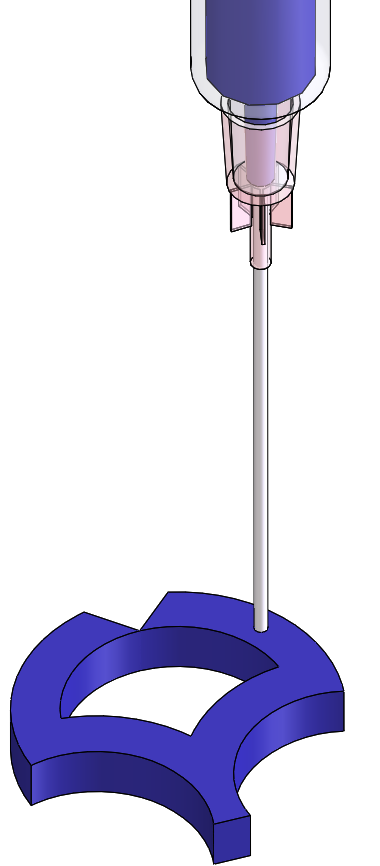
\includegraphics[trim = 0mm 0mm 0mm 0mm, clip, width=0.45in]{./images/OsakaU_logo.png}

\column{.85\textwidth}
\scalebox{0.85}{
\begin{tabular}{ c | c }
\textbf{Merit} & \textbf{Demerit} \\
\hline \hline
Affordable and scalable & Limited printing resolution and speed\\
Easy to set up and operate & Produce high stresses inside the needle\\
Deposit high cell densities & Low cell viability (40–80$\%$)
\end{tabular}
}
\end{columns}
\column{.25\textwidth}
\centering
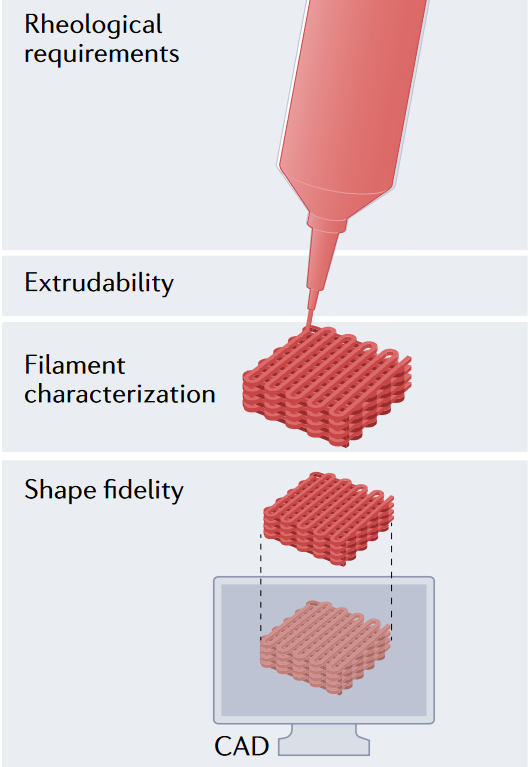
\includegraphics[trim = 0mm 0mm 0mm 0mm, clip, width=1.35in]{./images/intro.png}\\\tiny Assessment Criteria of 3D extrusion bioprinting.$^1$ \\ *CAD: computer-aided design.

\end{columns}
\footnotetext{\cite{zhang_3d_2021}}
\end{frame}


% 2 ---------------------------
\begin{frame}{Assessment Criteria}

\begin{columns}
\column{.45\textwidth}
\begin{itemize}
\setlength{\itemsep}{5mm}
\item Controlling stresses in the needle is a key factor to balance:
    \begin{itemize}
        \item Printing resolution
        \item Cell viability\footnotemark
    \end{itemize}
\item Printing efficiency
\begin{itemize}
    \item Extrusion speed
    \item Needle moving speed
\end{itemize}
\item Printability
    \begin{itemize}
        \item Extrudability
        \item Shape fidelity
    \end{itemize}
\end{itemize}

\column{.55\textwidth}
\begin{block}{Challenges:}
\begin{itemize}
    \item Difficult to experimentally observe stresses exerted on bioink inside the needle printhead.
    \item Testing thousands of different kinds of bioinks is a tedious and repetitive process.
    \item The need to optimize cell viability, printing efficiency, and printability.\footnotemark
\end{itemize}
\end{block}
\vspace{-3mm}
\begin{block}{Objective:}
\begin{itemize}
    \item Performing numerical simulation to understand and optimize needle geometries or bioink's rheological properties during the printing process to increase cell viability.
\end{itemize}
\end{block}
\end{columns}

\addtocounter{footnote}{-2}
\stepcounter{footnote}\footnotetext{\cite{blaeser_controlling_2016}}
\stepcounter{footnote}\footnotetext{\cite{zhang_direct_2020}}
\end{frame}


% 3 ---------------------------
\begin{frame}{Analytical Model of a Cylindrical Needle}

\small
\begin{columns}
\begin{column}{.4\textwidth}
\vspace{-0.5cm}
\begin{table}
\begin{tabular}{ c | c }
Symbol & Description \\
\hline \hline
$\tau_{rz}$ & Shear stress \\
$\eta$ & Apparent viscosity \\
$V_z$ &  Velocity along z-axis \\
$r$ & Variable radius \\
$K$ & Consistency index \\ 
$n$ & Flow index  \\
$\dot{\gamma}$ & Shear Rate  \\
$R$ & Needle radius \\
$P$ &  Pressure\\
$\Delta P_n$ &  Pressure drop in needle \\
$L_n$ & Needle length \\
$Q$ & Volumetric flow rate
\end{tabular}
%\caption{}
\end{table}
\end{column}

\begin{column}{.6\textwidth}
\begin{column}{.4\textwidth}
\begin{block}{Assumptions:}
\begin{enumerate}[I]\setlength{\itemsep}{0.01mm}
\setbeamertemplate{enumerate items}[square]
    \item Incompressible power-law fluid
    \item No-slip smooth wall boundary
    \item Negligible gravity influence
    \item Fully developed laminar flow
\end{enumerate}
\end{block}
\end{column}
\begin{column}{.6\textwidth}
\centering
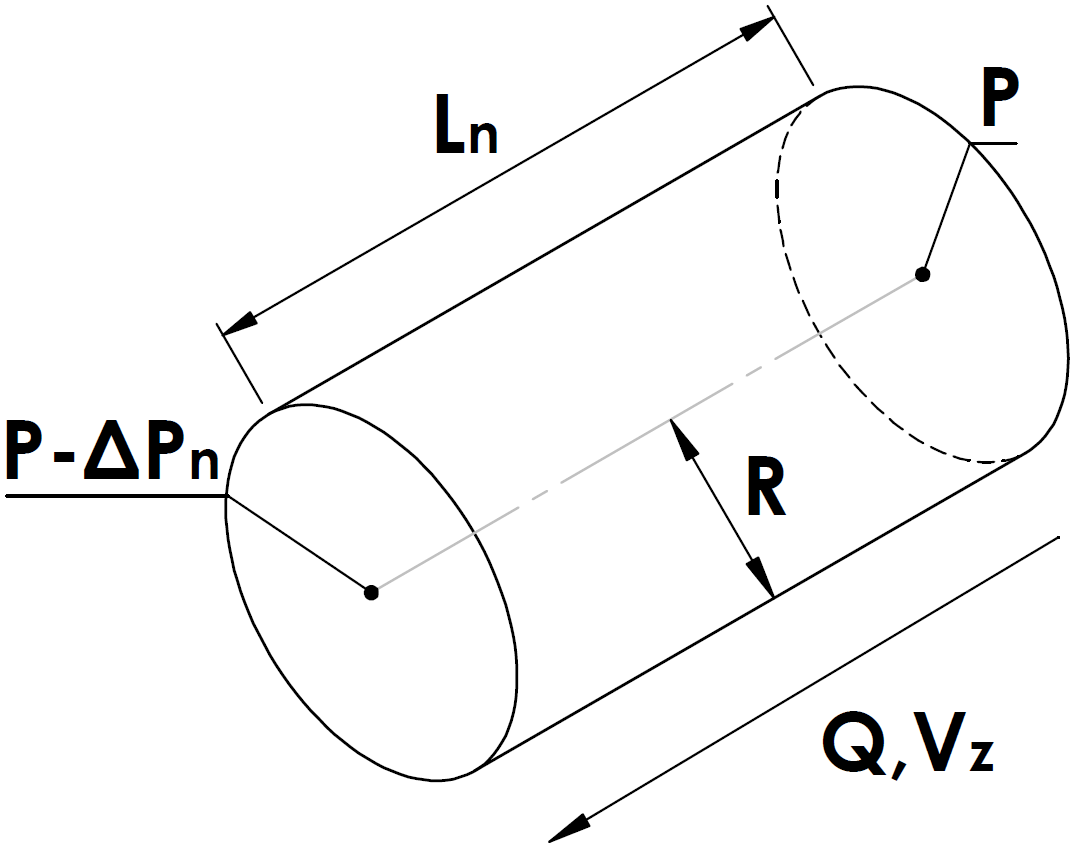
\includegraphics[trim = 0mm 0mm 0mm 0mm, clip, width=1.5in]{./images/math_model.png}\\\tiny Setup of analytical and simulation validations.

\end{column}
\vspace{-0.2cm}
\begin{equation*}
\tau_{rz} = \eta (\frac{\mathrm{d}V_z}{\mathrm{d}r}) = K\dot{\gamma}^n
%= (\frac{r}{2})(\frac{\Delta P_n}{L_n})
\end{equation*}
\vspace{-0.55cm}
\begin{equation*}
\eta = K\dot{\gamma}^{n-1}
\end{equation*}
\vspace{-0.55cm}
\begin{equation*}
V_z = \int_{r}^{R} \dot{\gamma} \,dr = R[1-(\frac{r}{R})^{\frac{n+1}{n}}](\frac{n}{n+1})(\frac{\Delta P_n R}{2KL_n})^{\frac{1}{n}}
\end{equation*}
\end{column}
\end{columns}

\end{frame}


% 4 ---------------------------
\begin{frame}{\openfoam Simulation Governing Equations}

\begin{columns}
\begin{column}{.5\textwidth}

\begin{itemize}
\item Incompressible continuity equation:
\end{itemize}
\begin{equation*}
\nabla \cdot \boldsymbol{U} = 0
\end{equation*}

\begin{itemize}
\item Steady-state Navier–Stokes equations:
\end{itemize}
\begin{equation*}
\boldsymbol{U}\cdot \nabla \boldsymbol{U}-\nabla \cdot (\frac{\eta}{\rho} \nabla \boldsymbol{U})=- \frac{\nabla P}{\rho}
\end{equation*}

\begin{itemize}
\item Poisson equation for pressure:
\end{itemize}
\begin{equation*}
\frac{\nabla^2 P}{\rho} = \nabla \cdot (\frac{\eta}{\rho}\nabla^2 \boldsymbol{U}-\boldsymbol{U}\cdot \nabla \boldsymbol{U})
\end{equation*}

\begin{itemize}
\item Power law modified Reynolds number:
\end{itemize}
\vspace{0.1cm}
\begin{equation*}
Re_{PL} = \frac{(2R)^n \bar{U}^{2-n}}{\frac{1}{\rho}K[(3n+1)/(4n)]^n 8^{n-1}}
\end{equation*}
\end{column}

\begin{column}{.5\textwidth}
\begin{itemize}
\item Shear rate (scalar):
\end{itemize}
\vspace{0.1cm}
\begin{equation*}
\dot{\gamma} = \sqrt{\frac{1}{2}\nabla \boldsymbol{U} : \nabla \boldsymbol{U}}
\end{equation*}

\begin{itemize}
\item Power law with a viscosity limiter:
\end{itemize}
\begin{equation*}
\eta = K\dot{\gamma}^{n-1},\ \eta_{\text{min}} \leq \eta \leq \eta_{\text{max}}
\end{equation*}

\def\arraystretch{1.2}%
\begin{table}
\begin{tabular}{ c | c }
Symbol & Description \\
\hline \hline
$\boldsymbol{U}$ & Velocity vector\\
$\bar{U}$ & Mean velocity\\
$\rho$ & Fluid density\\
$:$ & Inner product
\end{tabular}
%\caption{}
\end{table}
\end{column}
\end{columns}

\end{frame}


% 5 ---------------------------
\begin{frame}{Model Validation}

\begin{itemize}
\item \textbf{Setup}: 3D cylindrical needle ($R$ = 400 $\mu$m, $L_n$ = 13 mm, $Q$ = 50 $\mu$L/s)
\item \textbf{Alginate-based bioinks}: the most widely used commercial bioinks due to its low cost, biocompatibility, and facile gelation.\footnotemark
\item \textbf{Fluid properties}: 2.5$\%$ alginate (w/v) at 25 $^{\circ}$C ($K$ = 29.86 Pa$\cdot \text{s}^\text{n}$, $n$ = 0.46)
\end{itemize}

\begin{columns}
\small
\column{.64\textwidth}
\centering
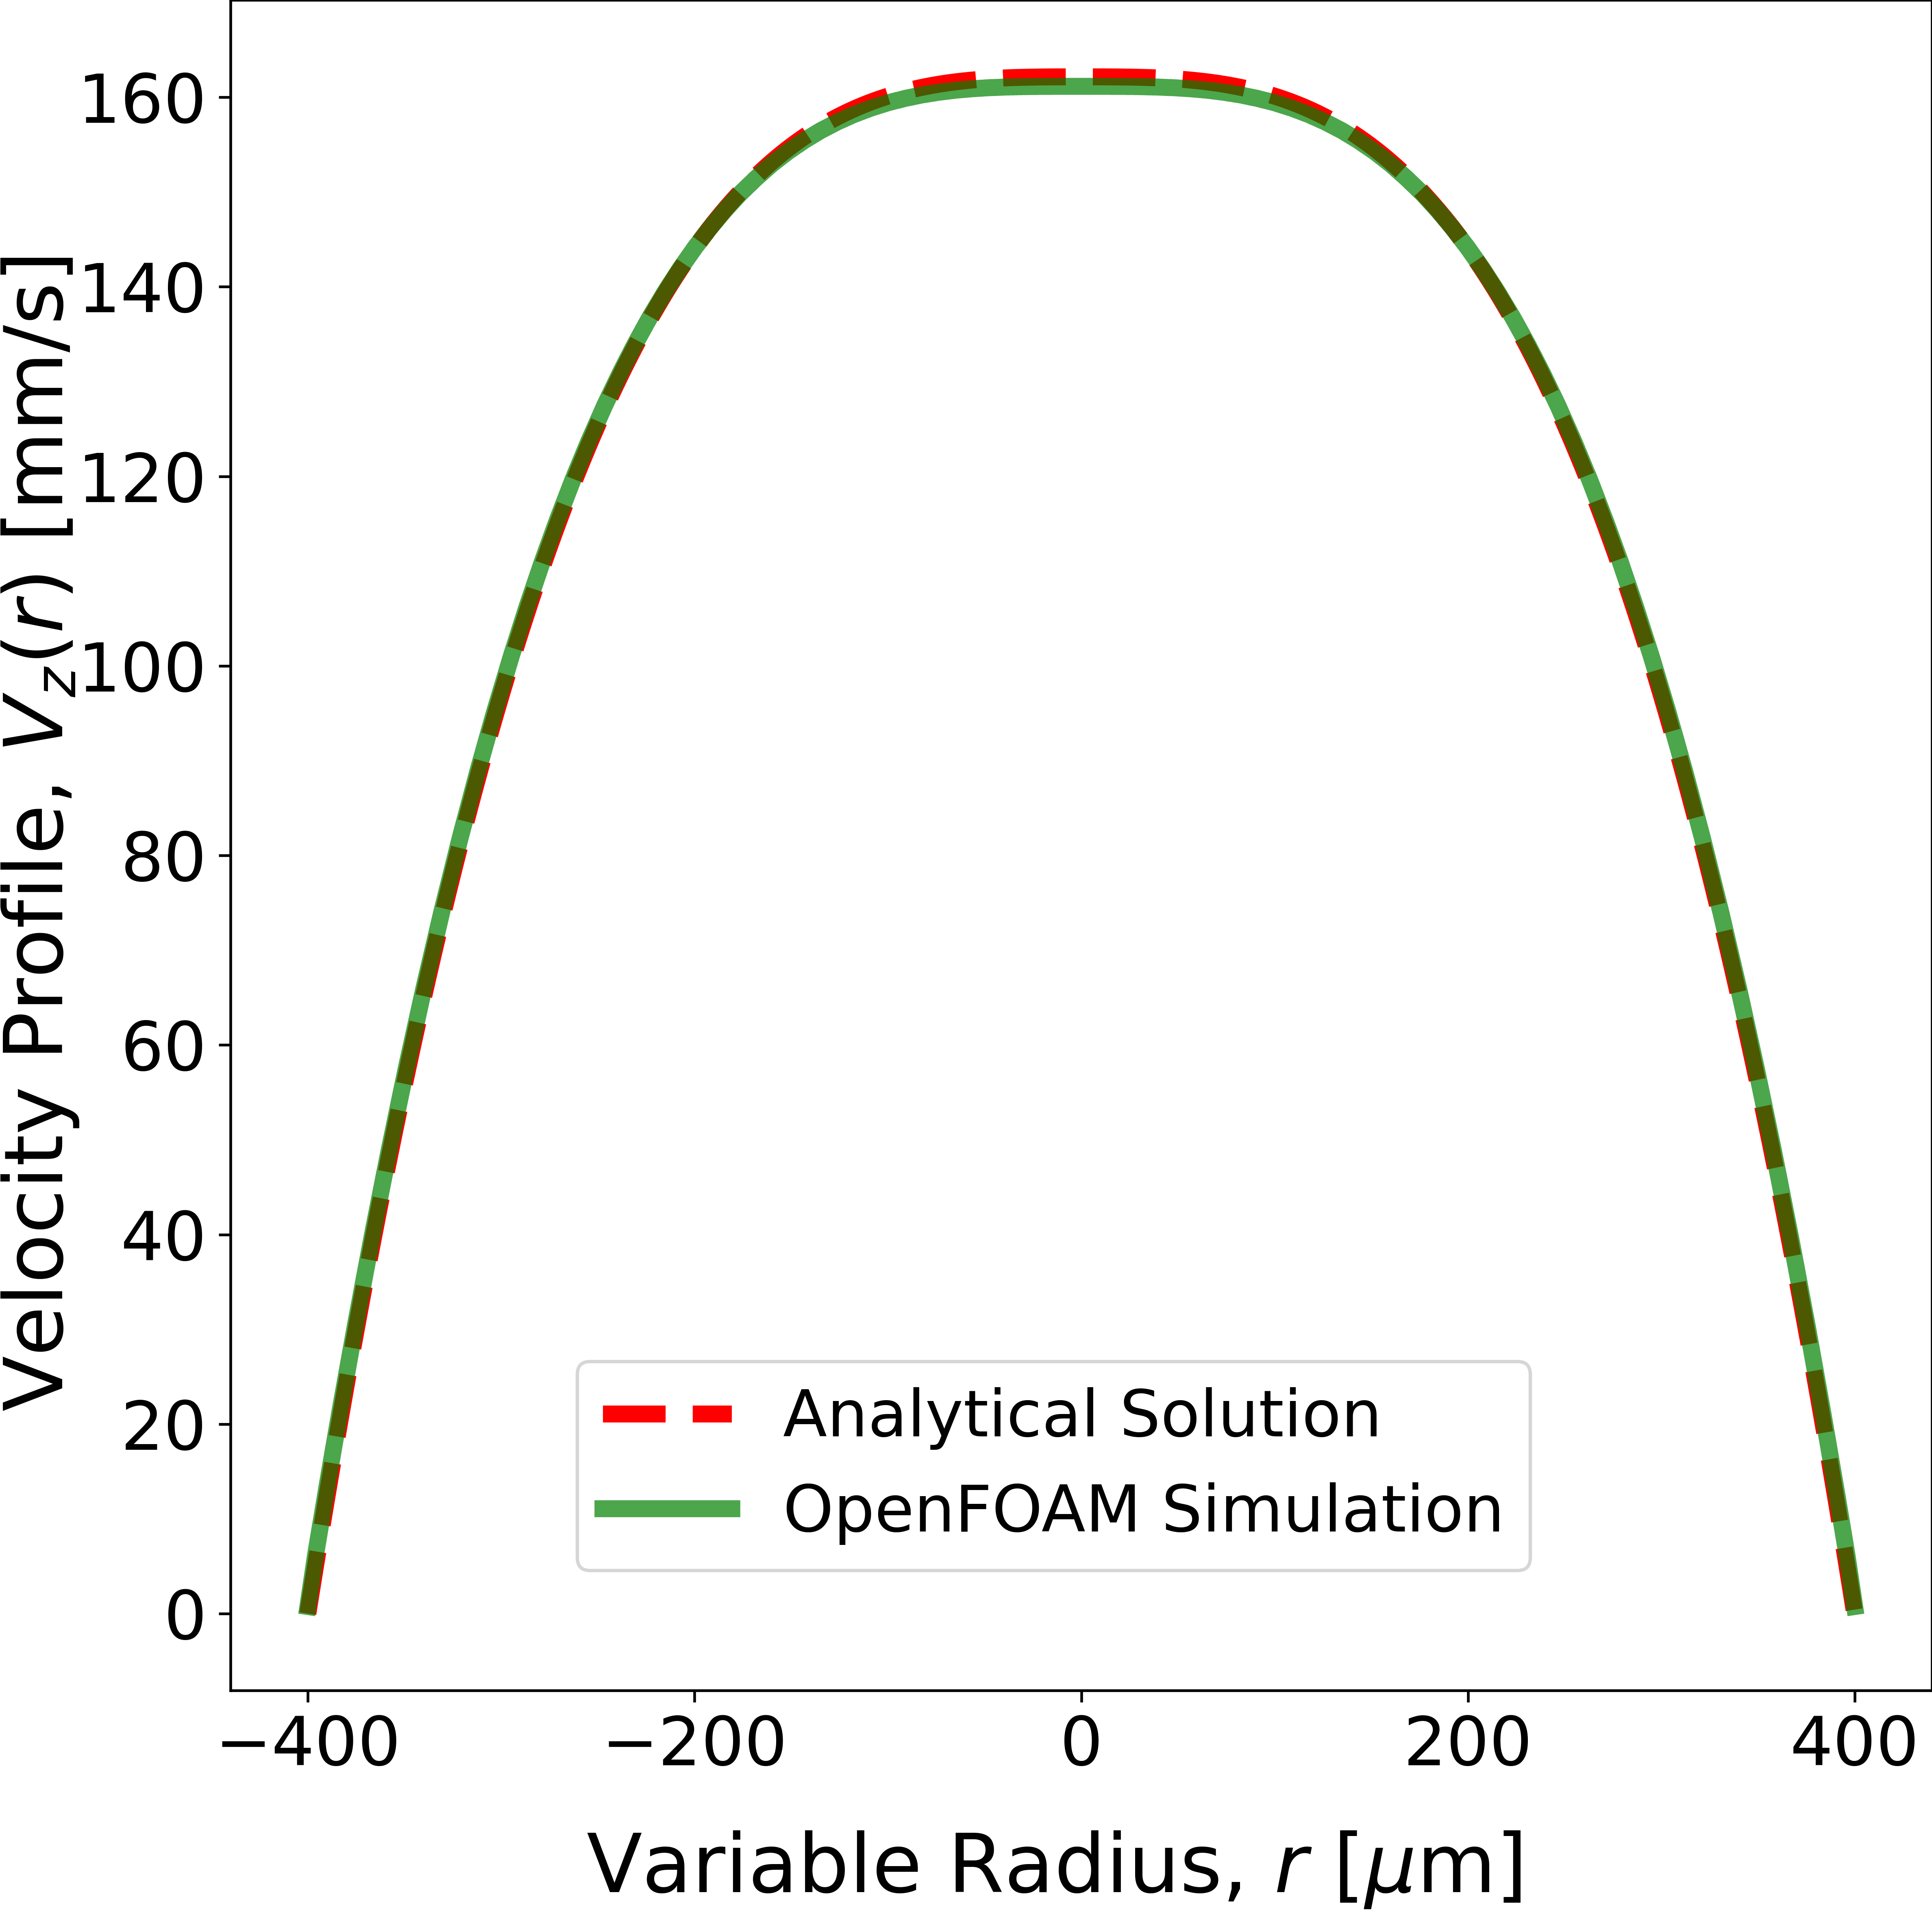
\includegraphics[trim = 0mm 0mm 0mm 0mm, clip, width=1.8in]{./images/velocity_profile.png}
\centering
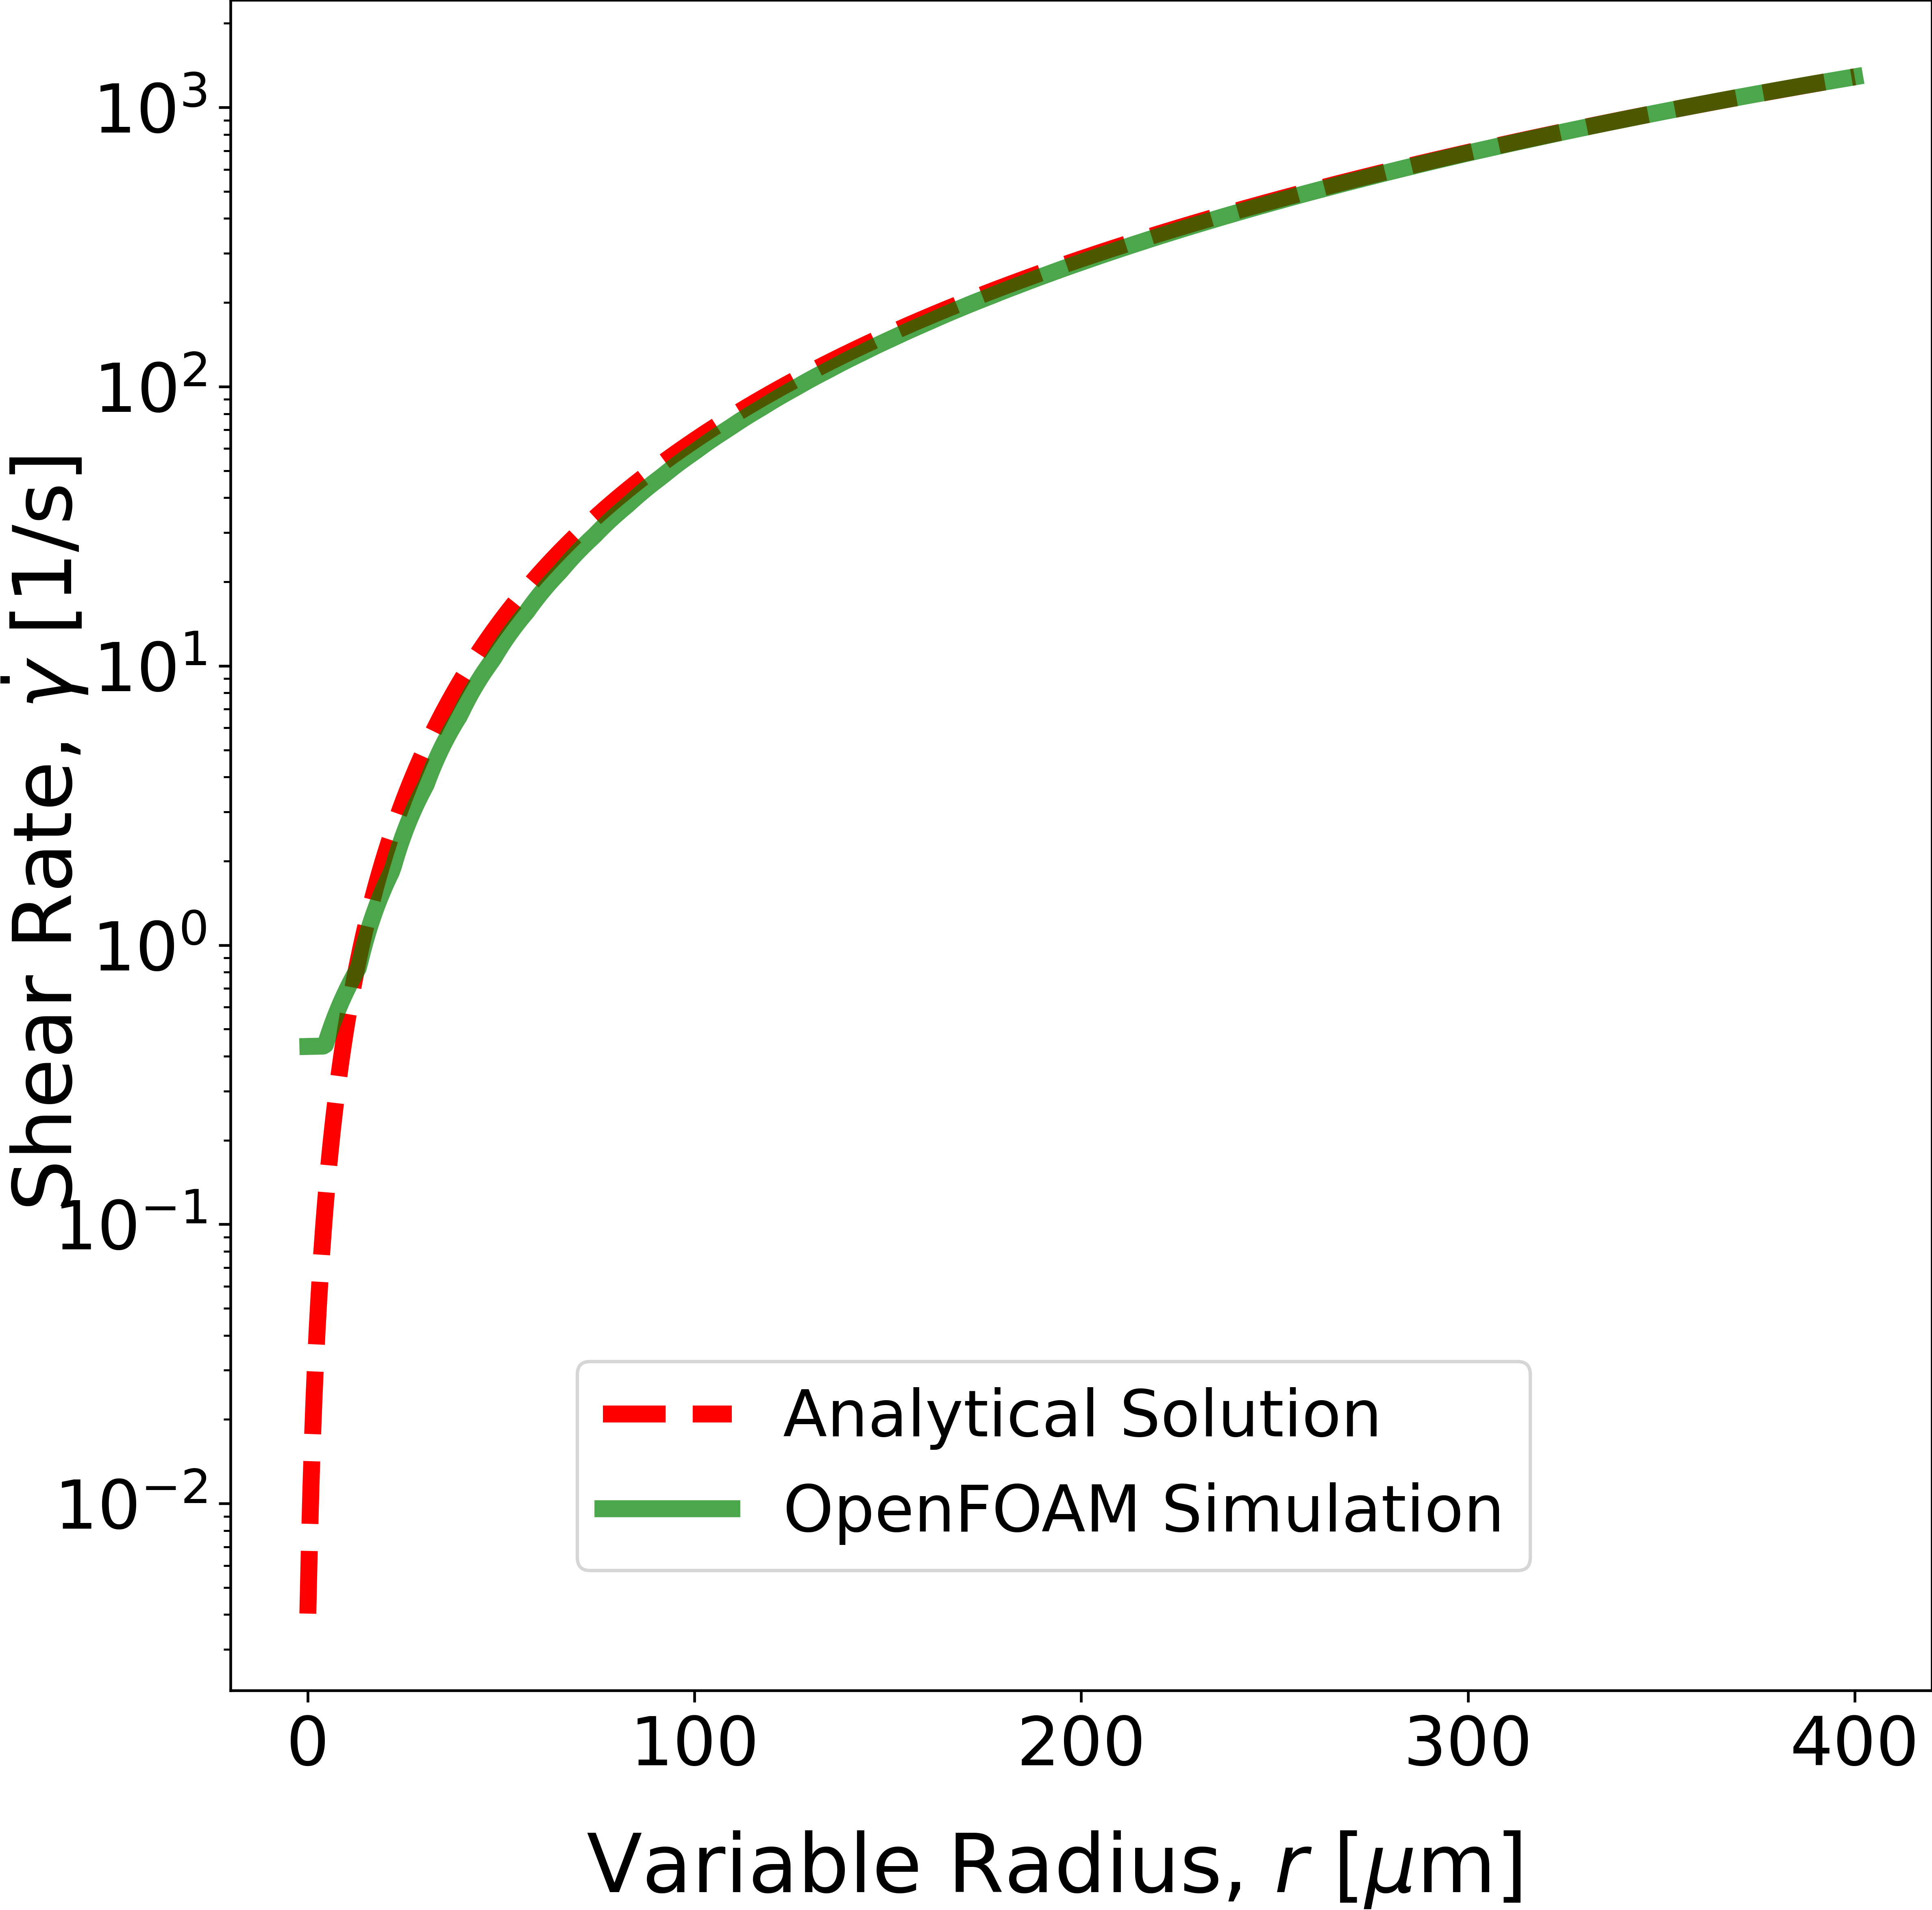
\includegraphics[trim = 0mm 0mm 0mm 0mm, clip, width=1.8in]{./images/shear_rate.png}

\column{.36\textwidth}
\begin{block}{}
    The analytical solution predicts a shear rate value of 0.0040 $\text{s}^{-1}$ at the center of the needle.
    
    However, the experimentally valid range for shear rates is between 0.1 and 1000 $\text{s}^{-1}$.
\end{block}
\end{columns}

\footnotetext{\cite{piras_multicomponent_2020}}
\end{frame}


% 6 ---------------------------
\begin{frame}{Model Validation Cont.}

\begin{columns}
\begin{column}{.5\textwidth}

\begin{itemize}
    \item The shear stress and shear rate showed strong correlation between analytical solution and simulation.
\end{itemize}
\vspace{3mm}
\centering
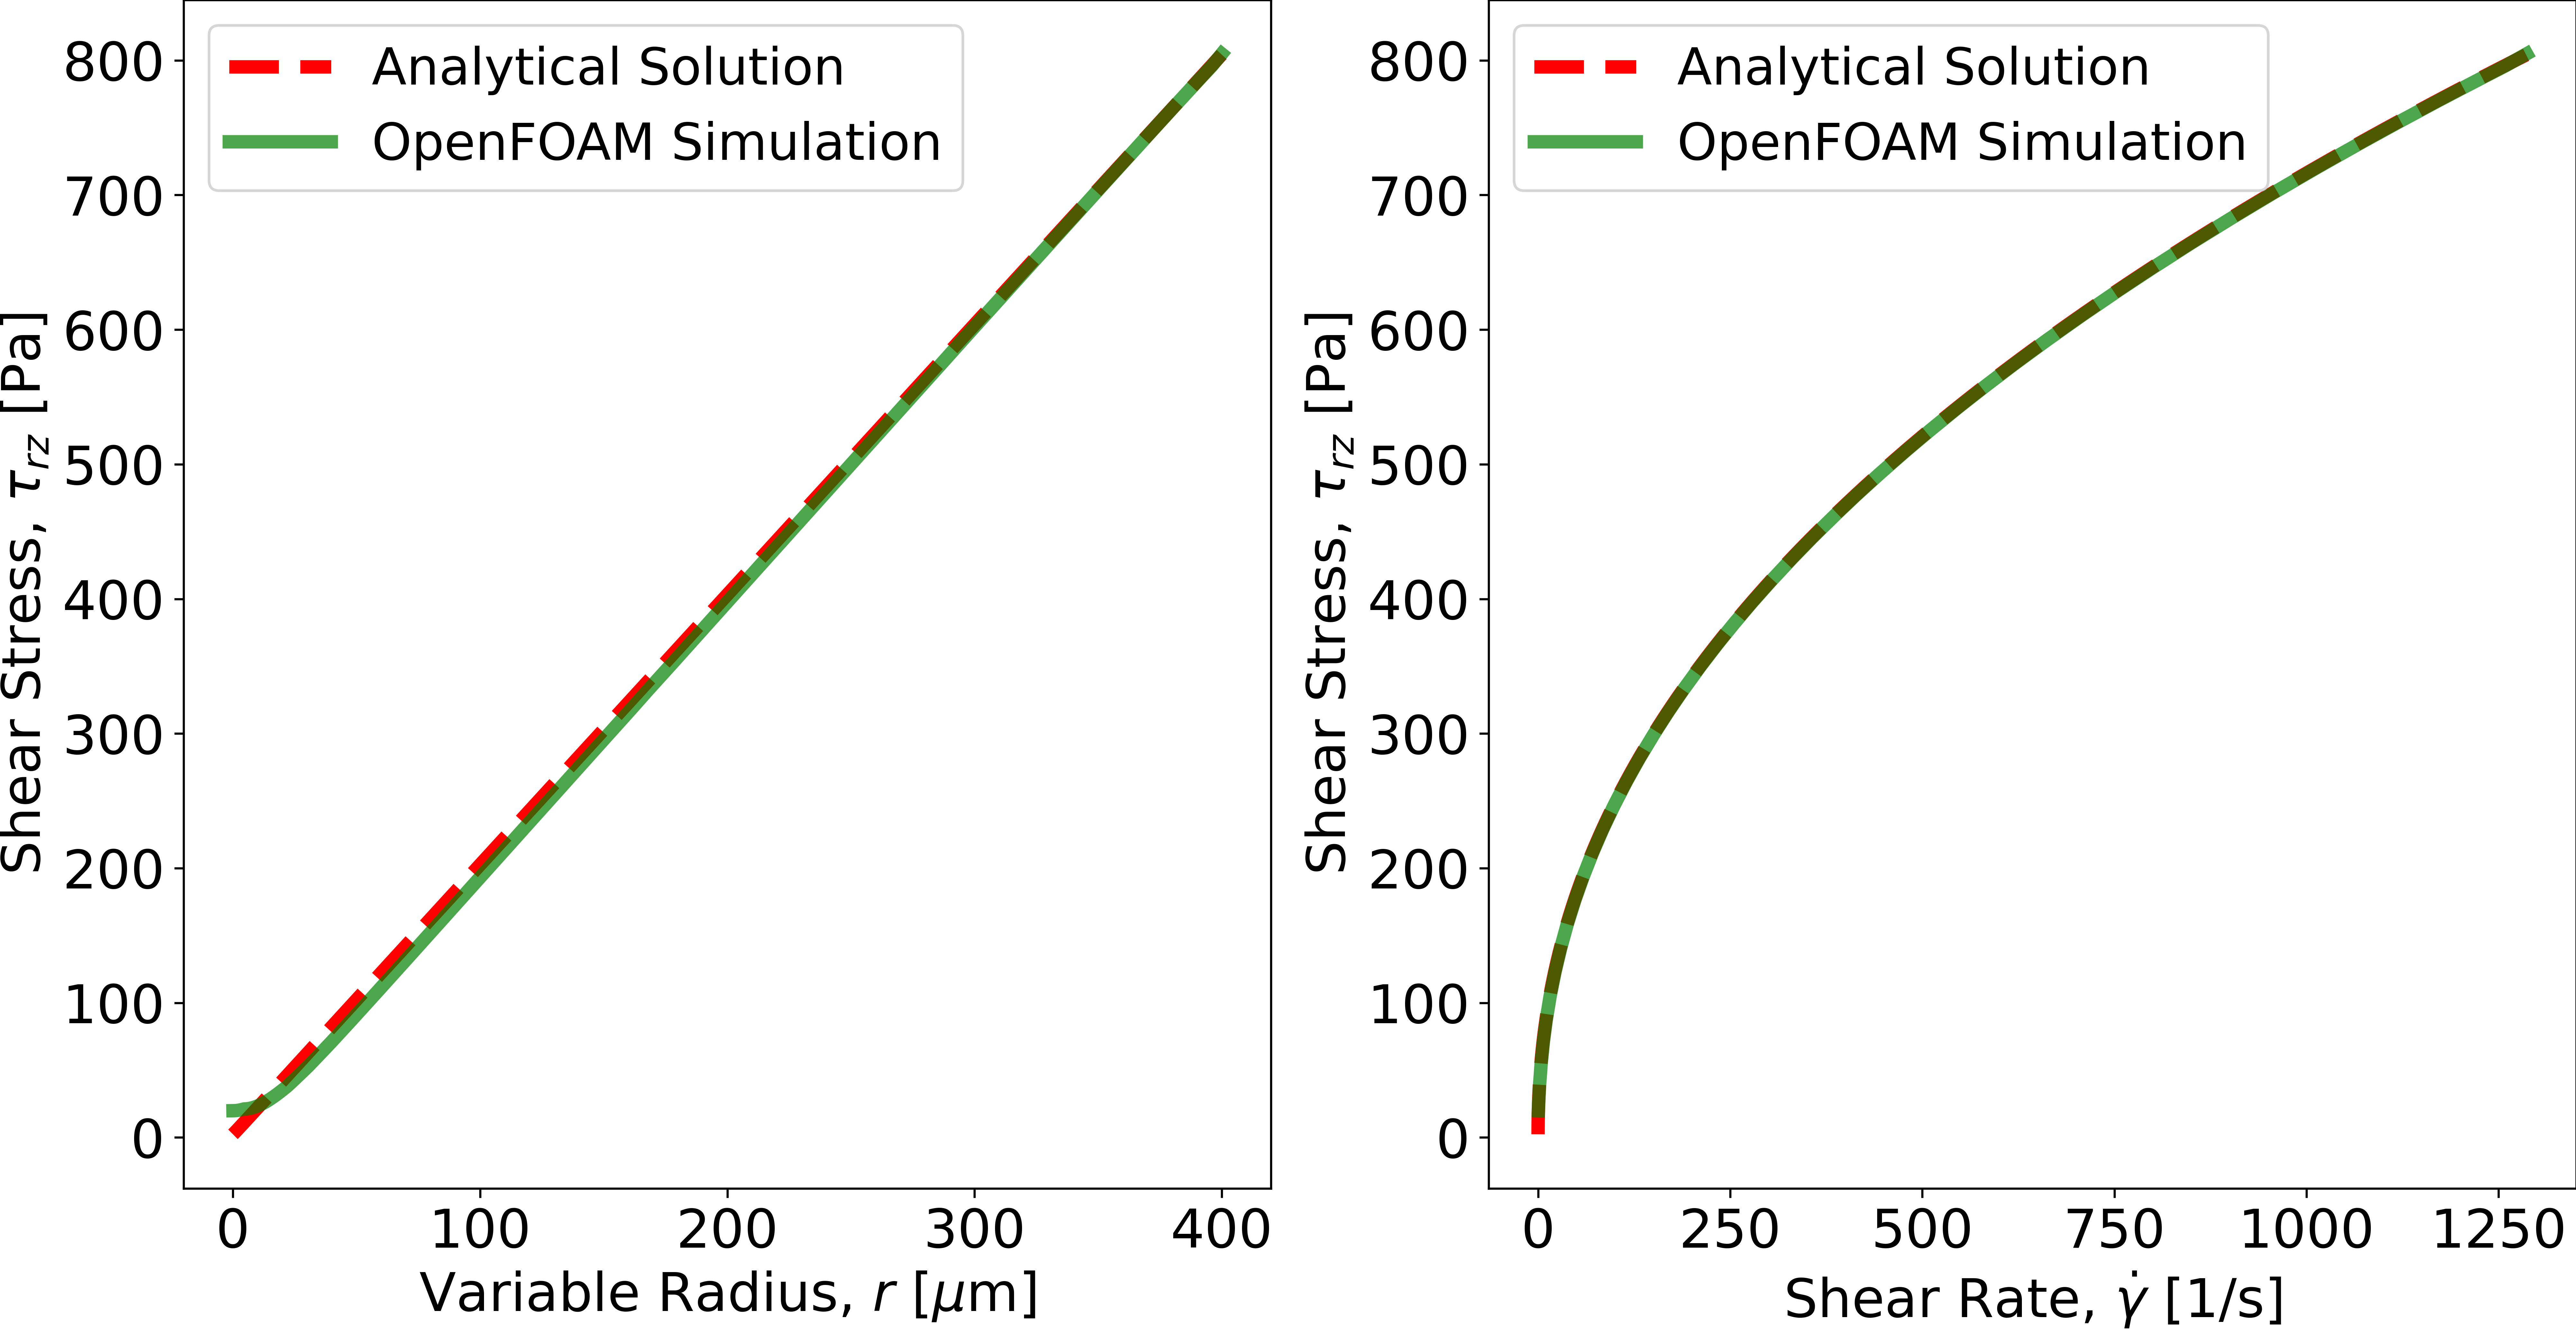
\includegraphics[trim = 0mm 0mm 0mm 0mm, clip, width=3.07in]{./images/shear_stress.png}
\end{column}

\begin{column}{.5\textwidth}
\begin{itemize}
    \item As the shear rate at the center of the needle didn't diverge in the simulation, apparent viscosities didn't diverge, too.
\end{itemize}
\vspace{3mm}
\centering
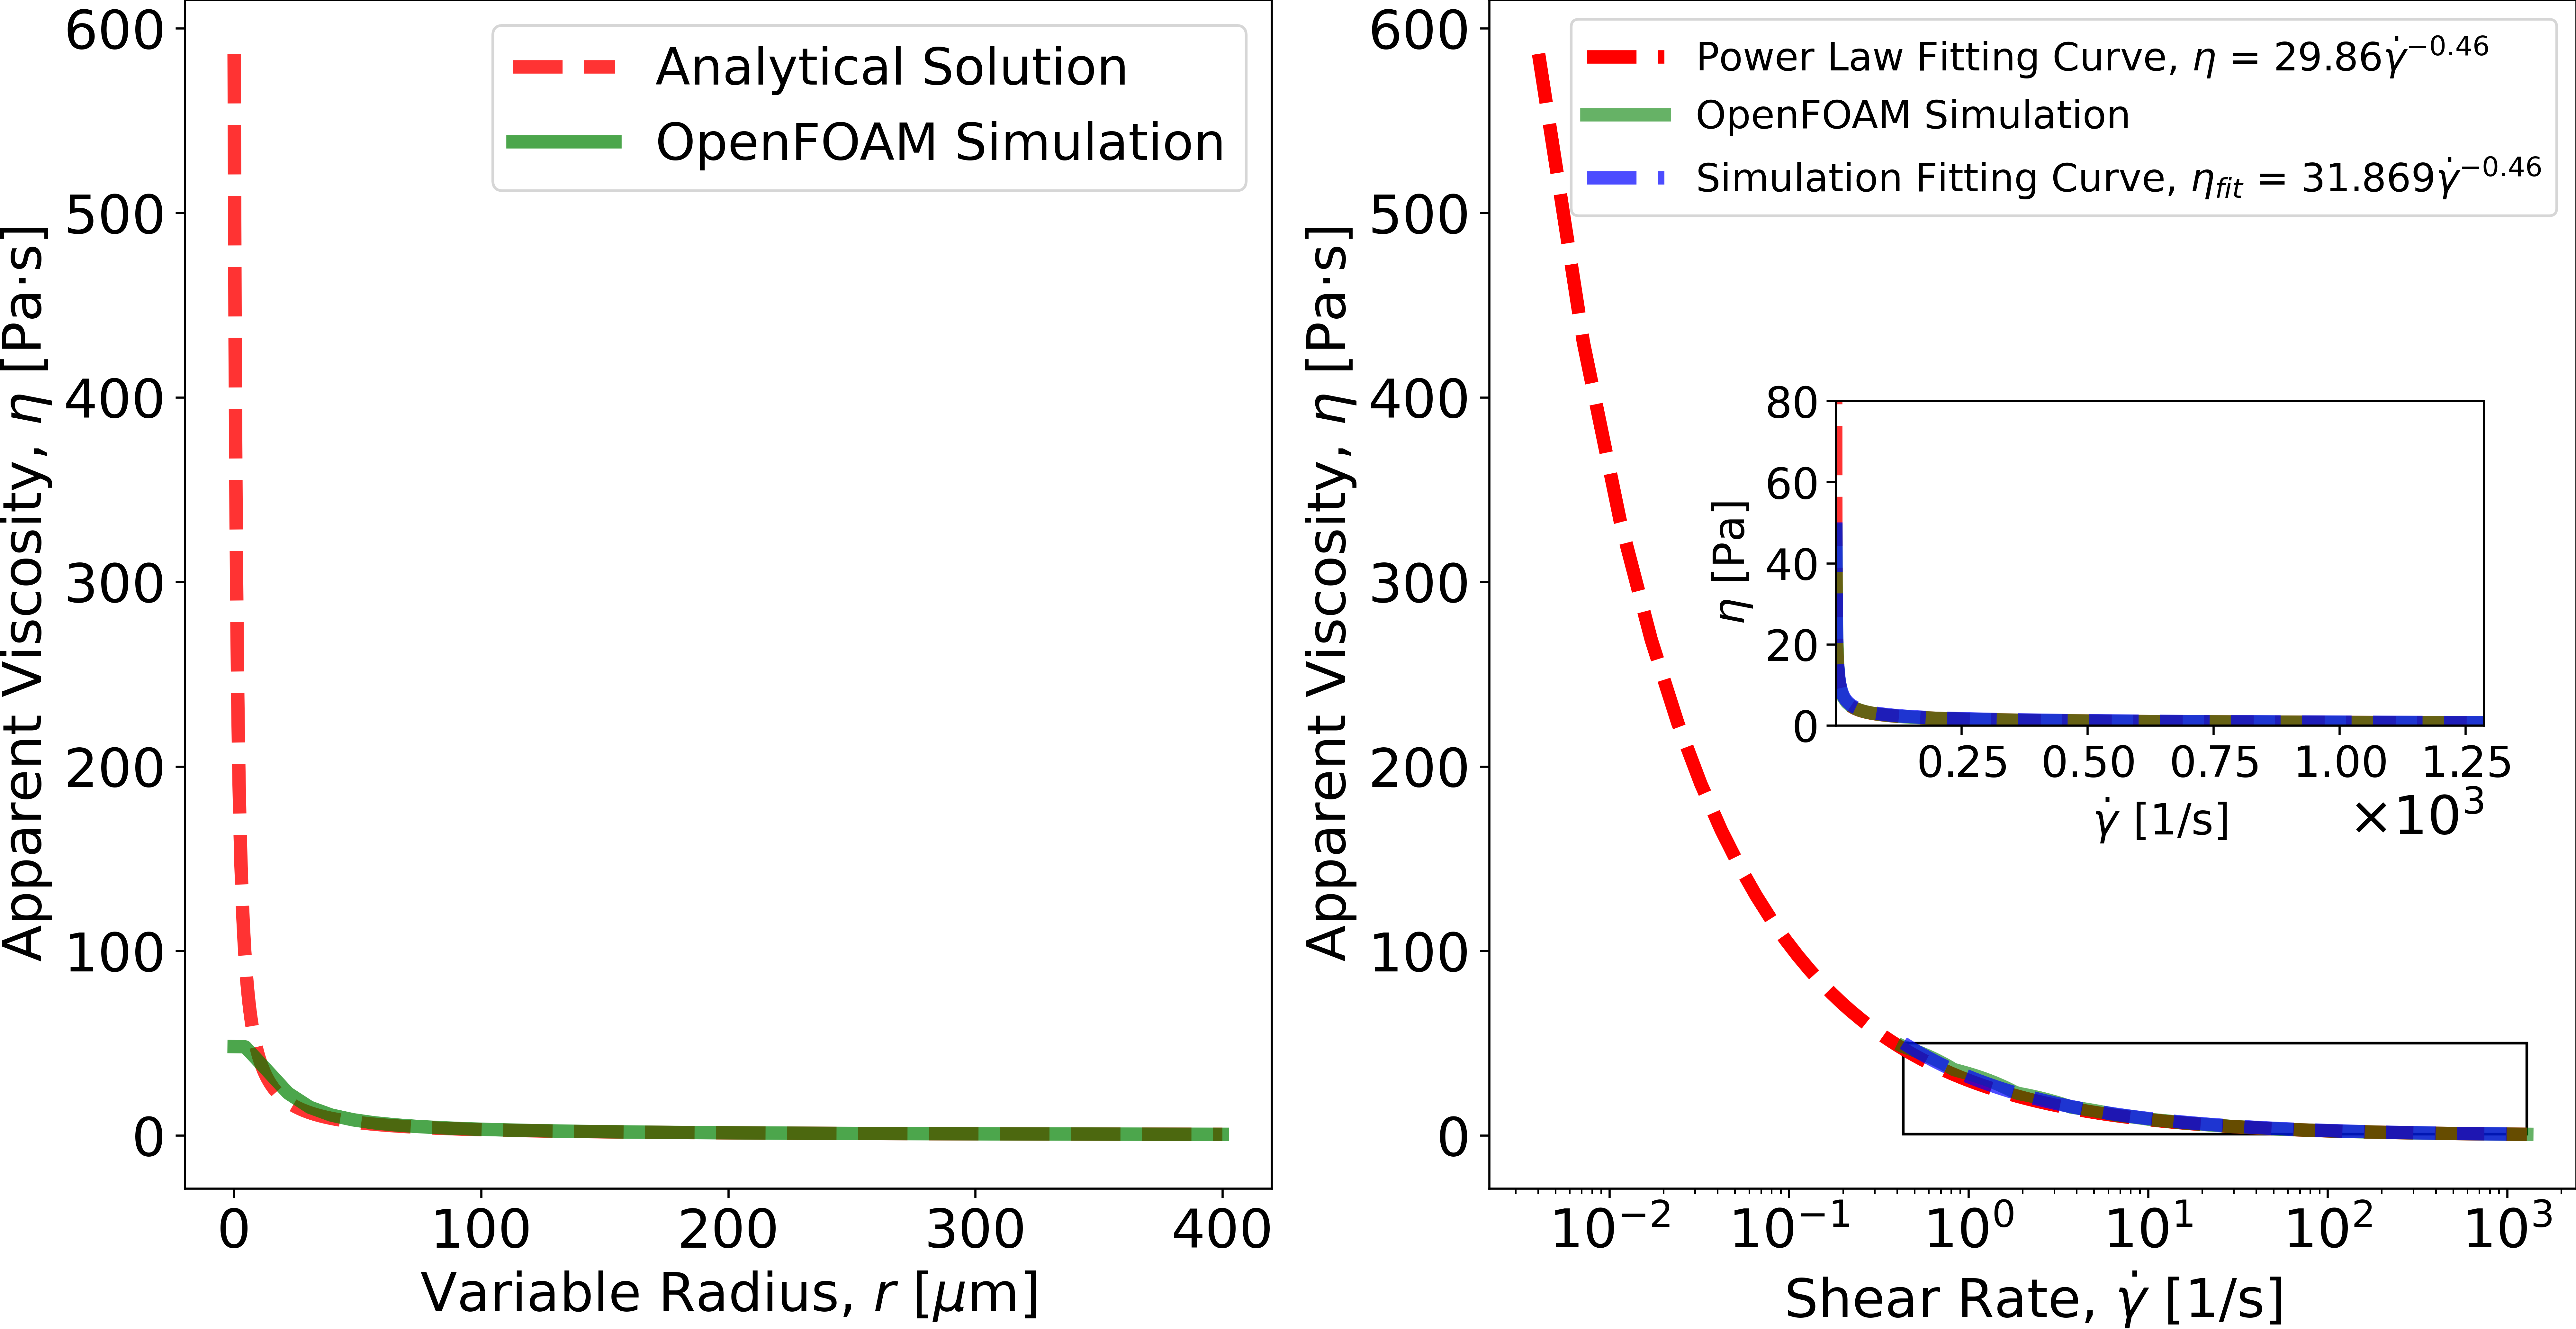
\includegraphics[trim = 0mm 0mm 0mm 0mm, clip, width=3.07in]{./images/apparent_viscosity.png}
\end{column}
\end{columns}

\end{frame}


% 7 ---------------------------
\begin{frame}{Needle Types and Assessment of Stresses}

\begin{itemize}
\setlength{\itemsep}{1mm}
\item Three types of needles are investigated ($L_n$ = 13 mm, $R$ = 400 $\mu$m; for tapered needle, $R$ ranges from 1850 $\mu$m to 400 $\mu$m).
\item Fluid properties are the same as before. Stresses (kPa) inside them are depicted.
\end{itemize}

\centering
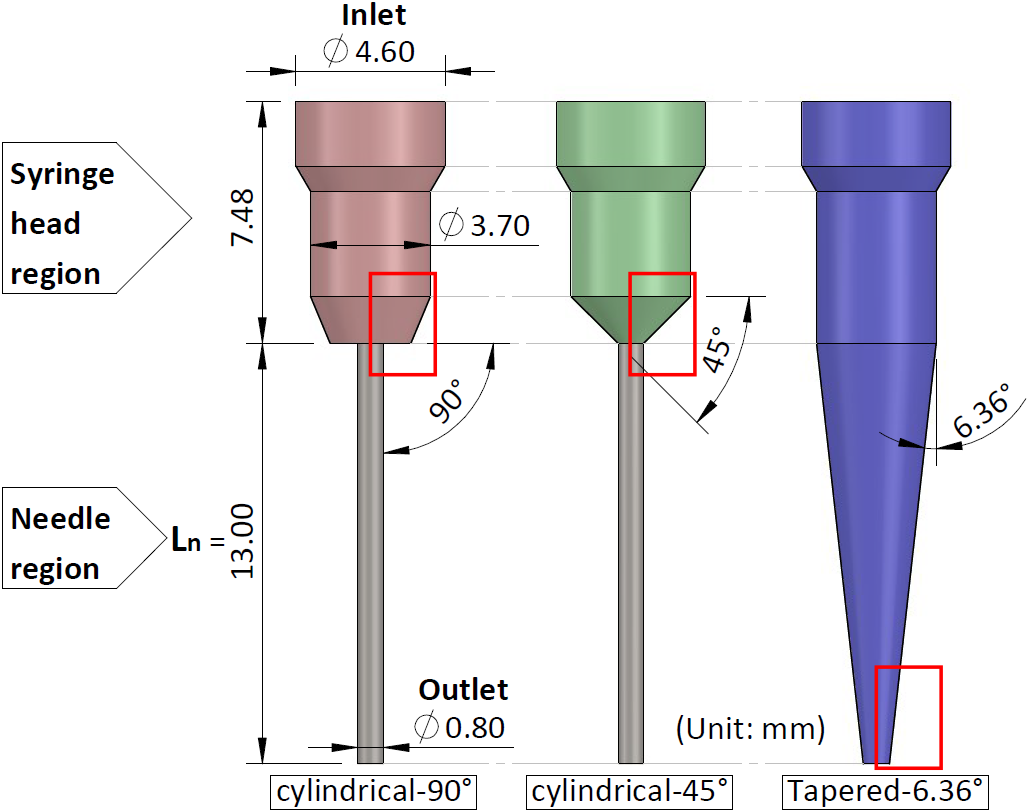
\includegraphics[trim = 0mm 0mm 0mm 0mm, clip, width=2.6in]{./images/needle_setup.png}
\centering
\setlength{\fboxrule}{1pt}
\setlength{\fboxsep}{1pt}
\fcolorbox{red}{white}{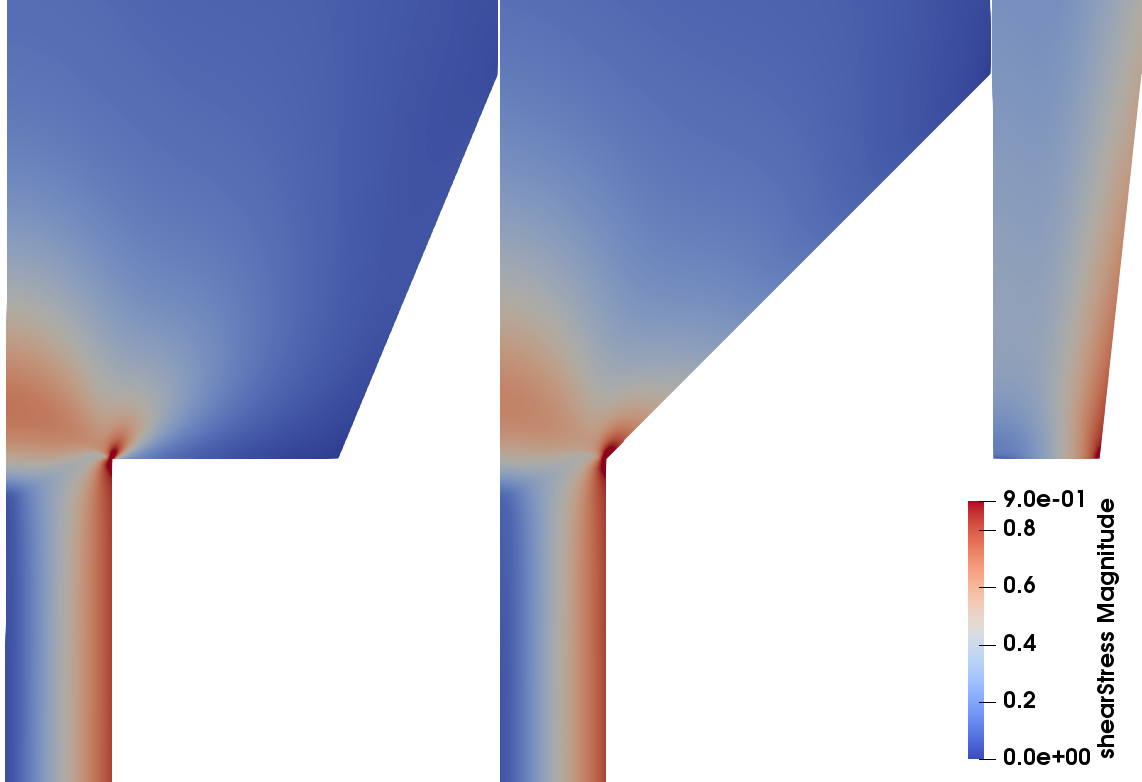
\includegraphics[trim = 0mm 0mm 0mm 0mm, clip, width=2.9in]{./images/needle_family_stress.png}}

\end{frame}


% 8 ---------------------------
\begin{frame}{Needle Types and Assessment of Stresses Cont.}

\begin{columns}
\begin{column}{.30\textwidth}
\begin{itemize}
    \item $\tau_{\text{max}} = $ 1.53 kPa
    \item $L_{\tau_{\text{max}}}$  $\approx$ 5 $\mu$m
    \item $\Delta P_n = 56.0$ kPa
    %\item $V_{z, \text{center}} = 162$ mm/s
    \item $\bar{\tau}_{\text{needle wall}} = 0.80$ kPa 
\end{itemize}
\vspace{1mm}
\centering
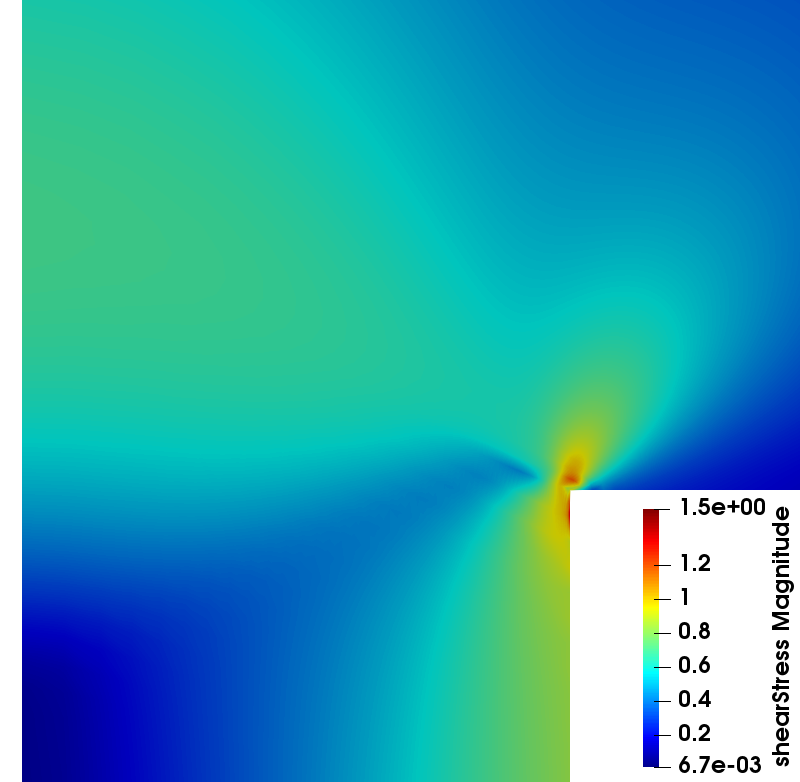
\includegraphics[trim = 0mm 0mm 0mm 50mm, clip, width=1.9in]{./images/needle_90_stress@25C.png}
\end{column}

\begin{column}{.30\textwidth}
\begin{itemize}
    \item $\tau_{\text{max}} = $ 1.48 kPa
    \item $L_{\tau_{\text{max}}}$  $\approx$ 15 $\mu$m
    \item $\Delta P_n = 55.2$ kPa
    %\item $V_{z, \text{center}} = 163$ mm/s
    \item $\bar{\tau}_{\text{needle wall}} = 0.80$ kPa 
\end{itemize}
\vspace{1mm}
\centering
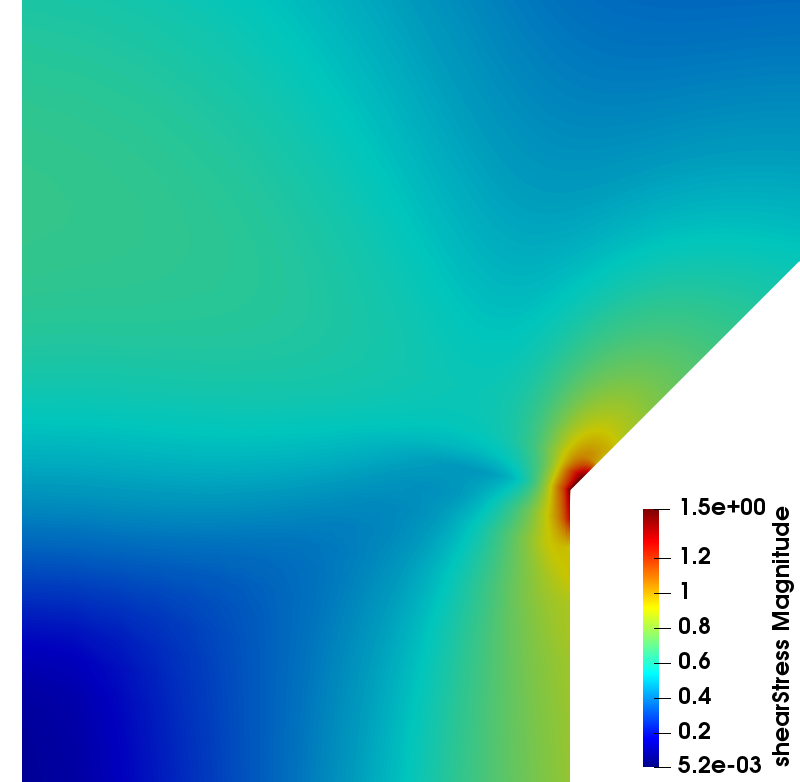
\includegraphics[trim = 0mm 0mm 0mm 50mm, clip, width=1.9in]{./images/needle_45_stress@25C.png}
\end{column}

\begin{column}{.36\textwidth}
\begin{itemize}
    \item $\tau_{\text{max}} = $ 1.11 kPa
    \item $L_{\tau_{\text{max}}}$  $\approx$ 20 $\mu$m
    \item $\Delta P_n = 10.1$ KPa
    %\item $V_{z, \text{center}} = 13.0$–$150$ mm/s
    \item $\tau_{\text{needle wall}} = 0.063$–$1.1$ kPa 
\end{itemize}
\vspace{1mm}
\centering
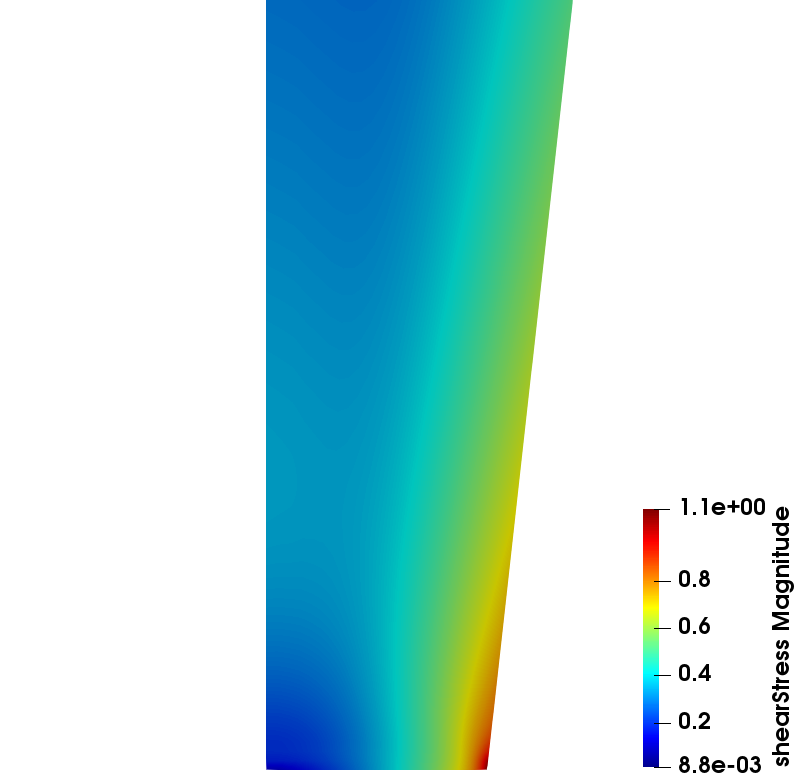
\includegraphics[trim = 0mm 0mm 0mm 50mm, clip, width=1.9in]{./images/needle_tapered_stress@25C.png}
\end{column}
\end{columns}

\end{frame}


% 9 ---------------------------
\begin{frame}{Temperature Dependency of Bioinks' Rheological Properties}

\small
\begin{itemize}
    \item Experimental data on $2.5\%$ alginate (w/v) under various temperatures (error or uncertainty not shown on the table)\footnotemark:
\end{itemize}
\begin{center}
Apparent viscosity: $\eta = K\dot{\gamma}^{n-1}$
  % Command to increase the spacing(stretching) between terms in the table.
  \renewcommand{\arraystretch}{1.2}
  \begin{tabular}{ c c c c c c}
    \hline
    Temperature ($^{\circ}$C) & 25 & 35 & 45 & 55 \\ \hline
    $K$ (Pa$\cdot \text{s}^\text{n}$) & 29.86 & 18.50 & 12.53 & 5.13 \\
    $n$ (-) & 0.46 & 0.51 & 0.56 & 0.64 \\
  \hline
  \end{tabular}
\end{center}
\vspace{-0.1cm}
\begin{itemize}
    \item Temperature change has a significant impact on the viscosity of $2.5\%$ alginate (w/v).
    \begin{itemize}
        \setlength{\itemsep}{2mm}
        \item As temperature $\Uparrow$, $K$ $\Downarrow$ and $n$ $\Uparrow$; kept flow rate, $Q$, constant, and $\dot{\gamma}_\text{max}$ $\Downarrow$, $\dot{\gamma}_\text{min}$ $\Uparrow$.
        \item As $K$ $\Downarrow$, apparent viscosity, $\eta$ $\Downarrow$.
        \item As $n$ $\Uparrow$, the fluid behaves more and more Newtonian, and apparent viscosity, $\eta$ $\Downarrow$.
    \end{itemize}
    \item A significant reduction in stresses is expected, as apparent viscosity, $\eta$ $\Downarrow$$\Downarrow$.
\end{itemize}

\footnotetext{\cite{sarker_modeling_2017}}
\end{frame}


% 10 ---------------------------
\begin{frame}{Viscosity under the influence of Temperature Changes}

\footnotesize
\begin{itemize}
    \item Apparent viscosities, $\eta$, are highest at the needle centers. As temperature $\Uparrow$, $\eta$ $\Downarrow$ nonlinearly, indicating a nonlinear relationship between apparent viscosity and temperature.
\end{itemize}
\vspace{-3.5mm}
\begin{columns}
\begin{column}{.333\textwidth}
\begin{itemize}
    \item 90$^{\circ}$ cylindrical needle:
\end{itemize}
\vspace{0.5mm}
\centering
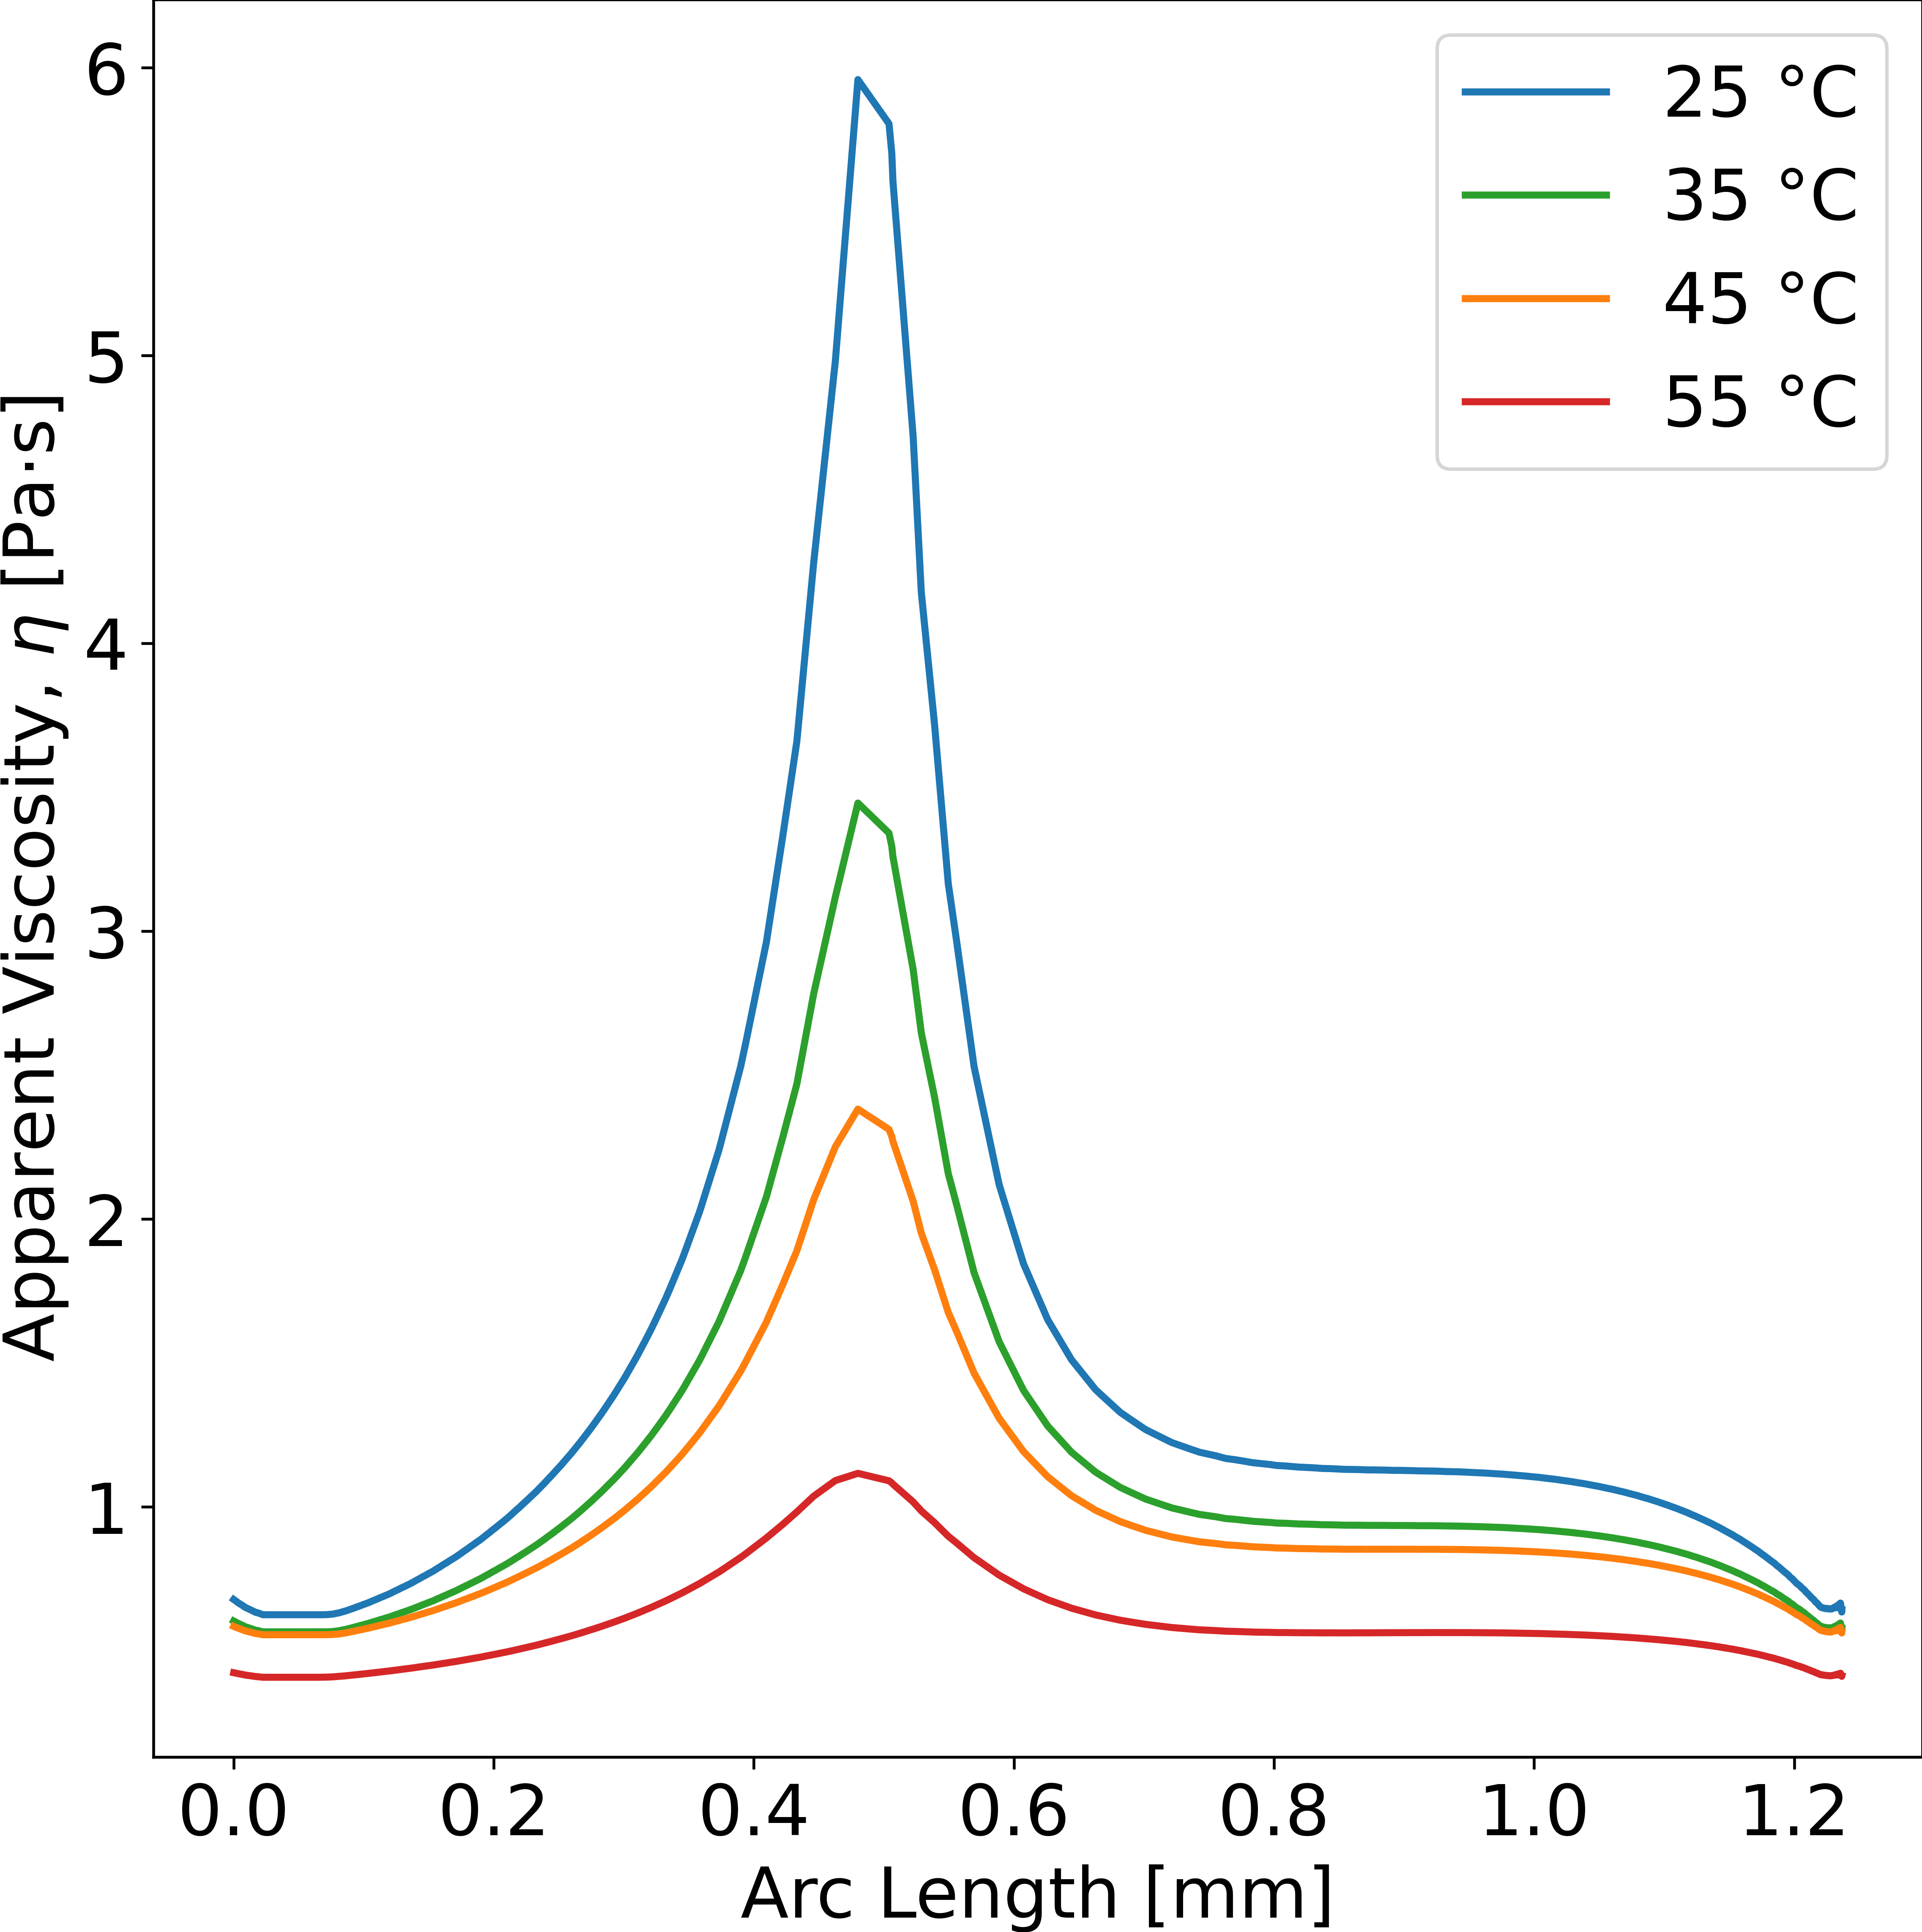
\includegraphics[trim = 0mm 0mm 0mm 0mm, clip, width=1.9in]{./images/90_nudata_sphere.png}
\end{column}

\begin{column}{.333\textwidth}
\begin{itemize}
    \item 45$^{\circ}$ cylindrical needle:
\end{itemize}
\vspace{0.5mm}
\centering
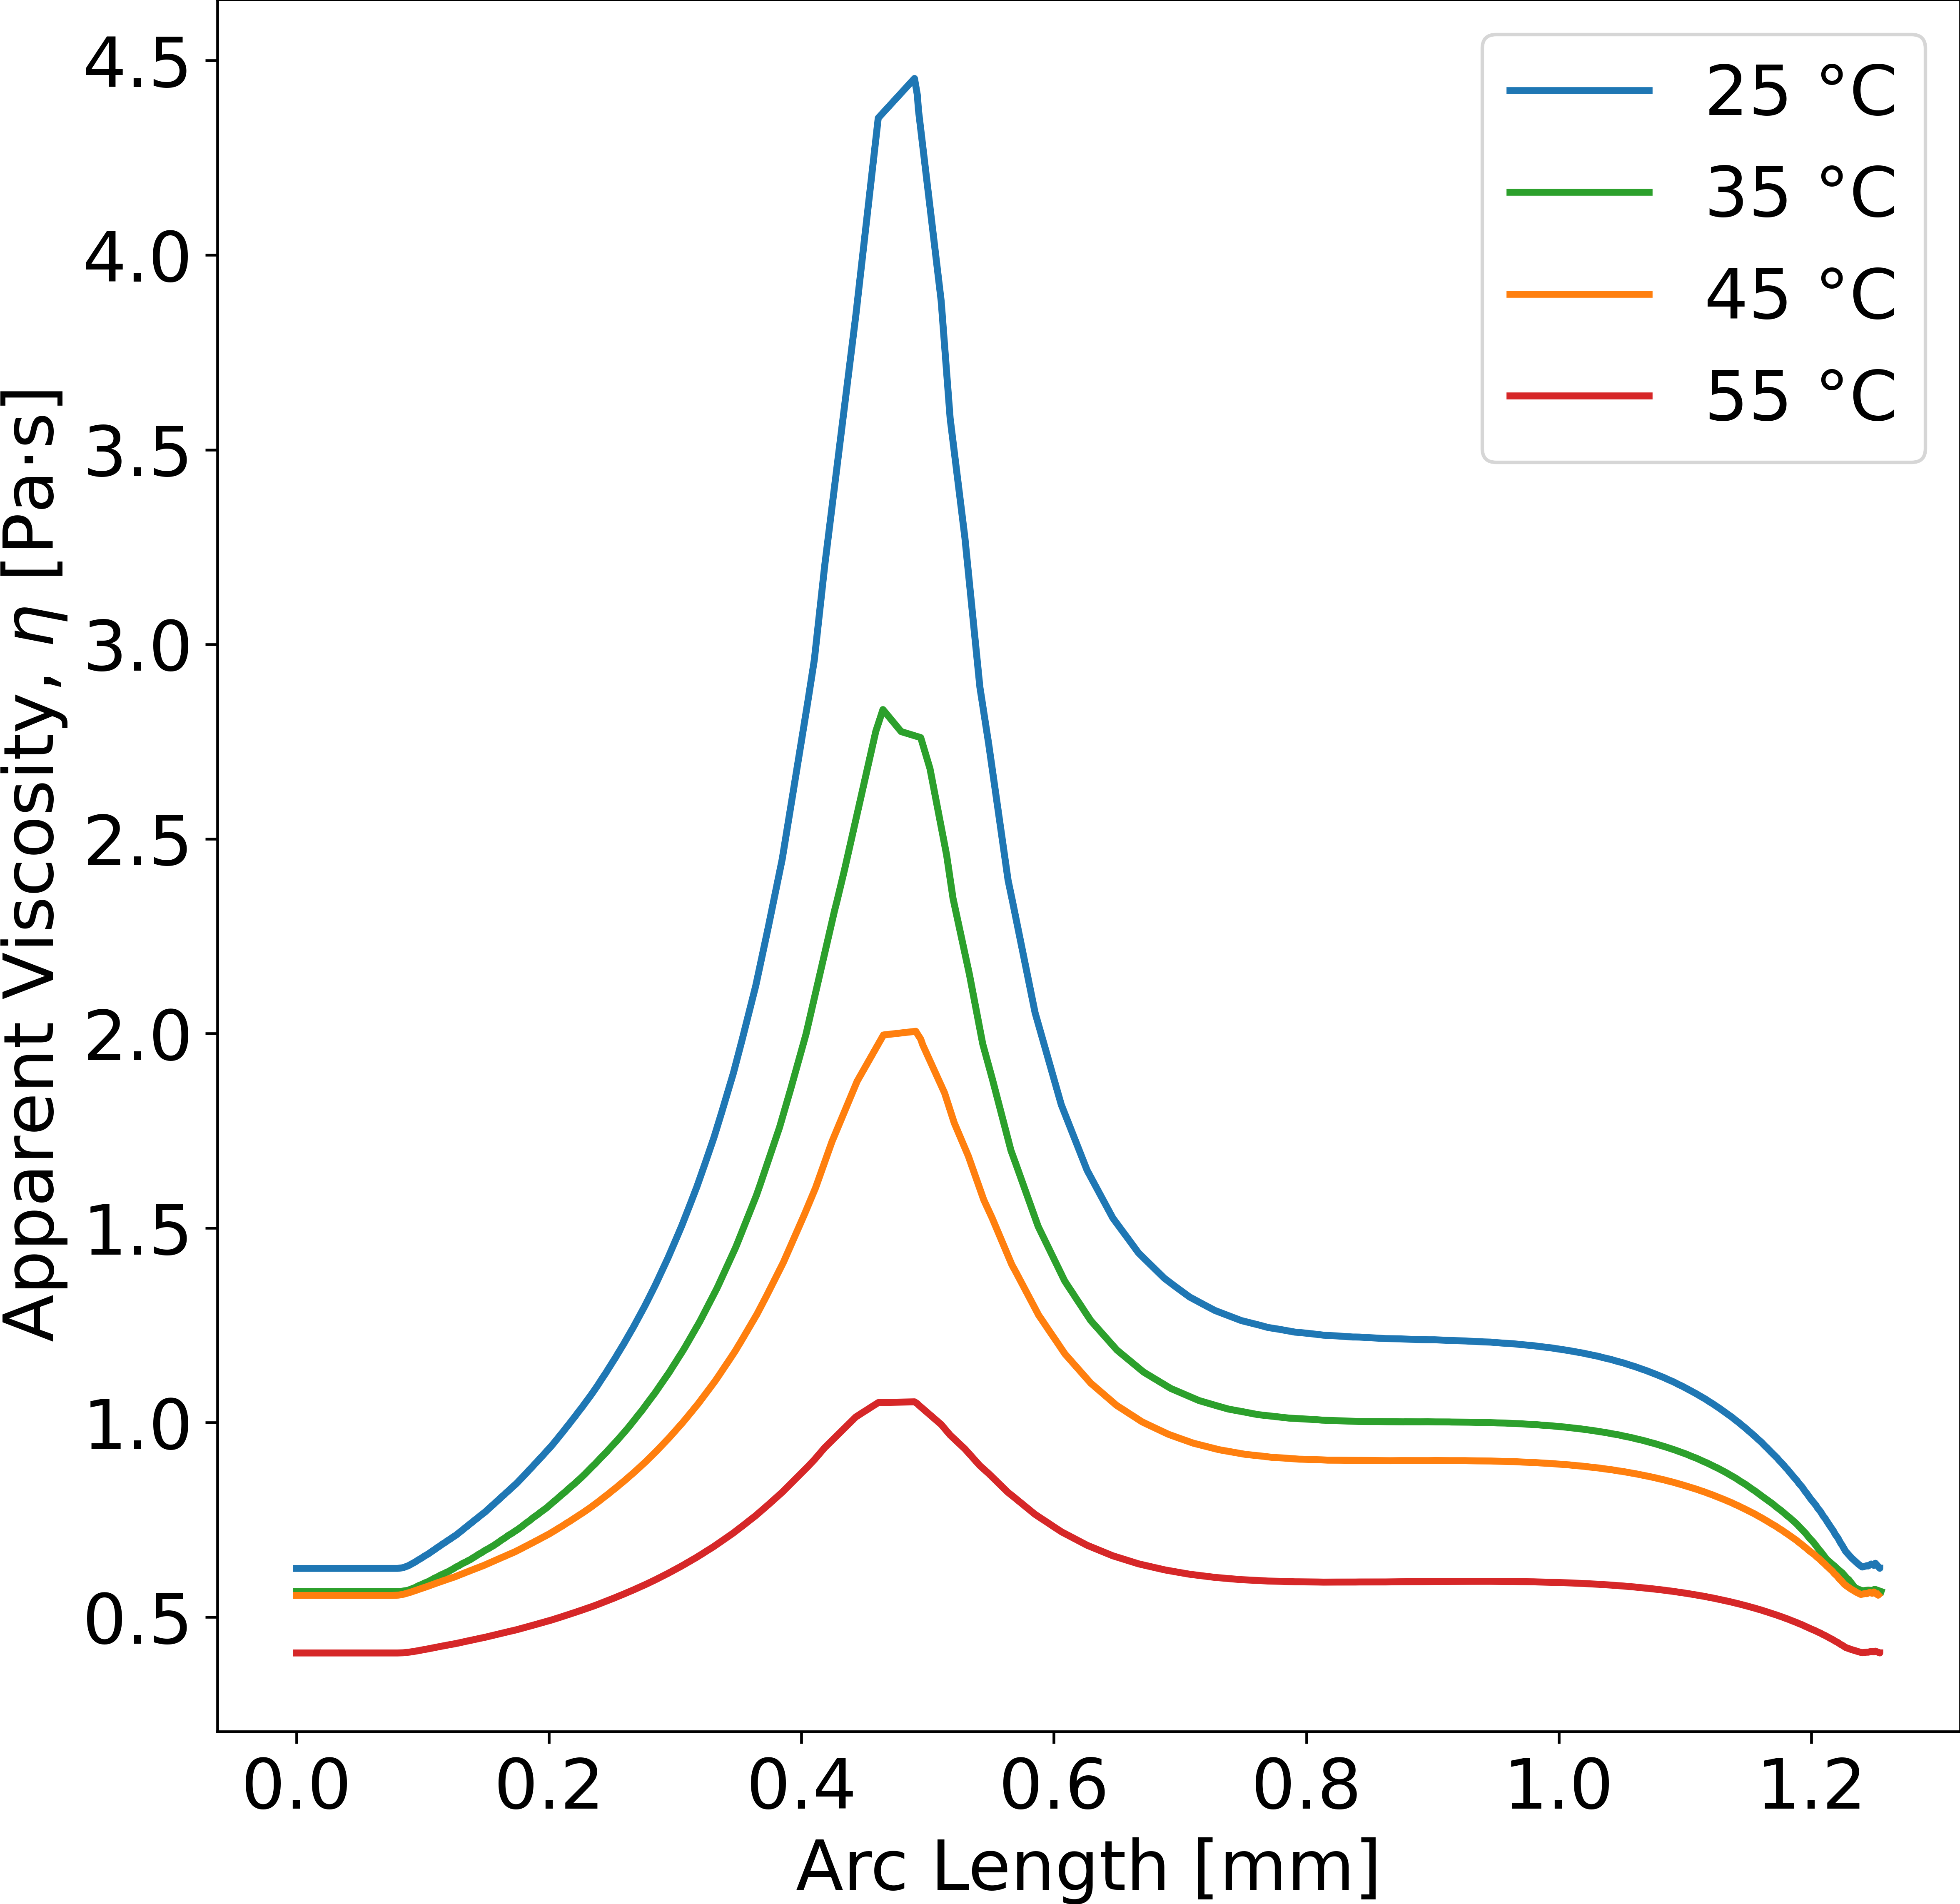
\includegraphics[trim = 0mm 0mm 0mm 0mm, clip, width=1.98in]{./images/45_nudata_sphere.png}
\end{column}

\begin{column}{.333\textwidth}
\begin{itemize}
    \item Tapered needle:
\end{itemize}
\vspace{0.5mm}
\centering
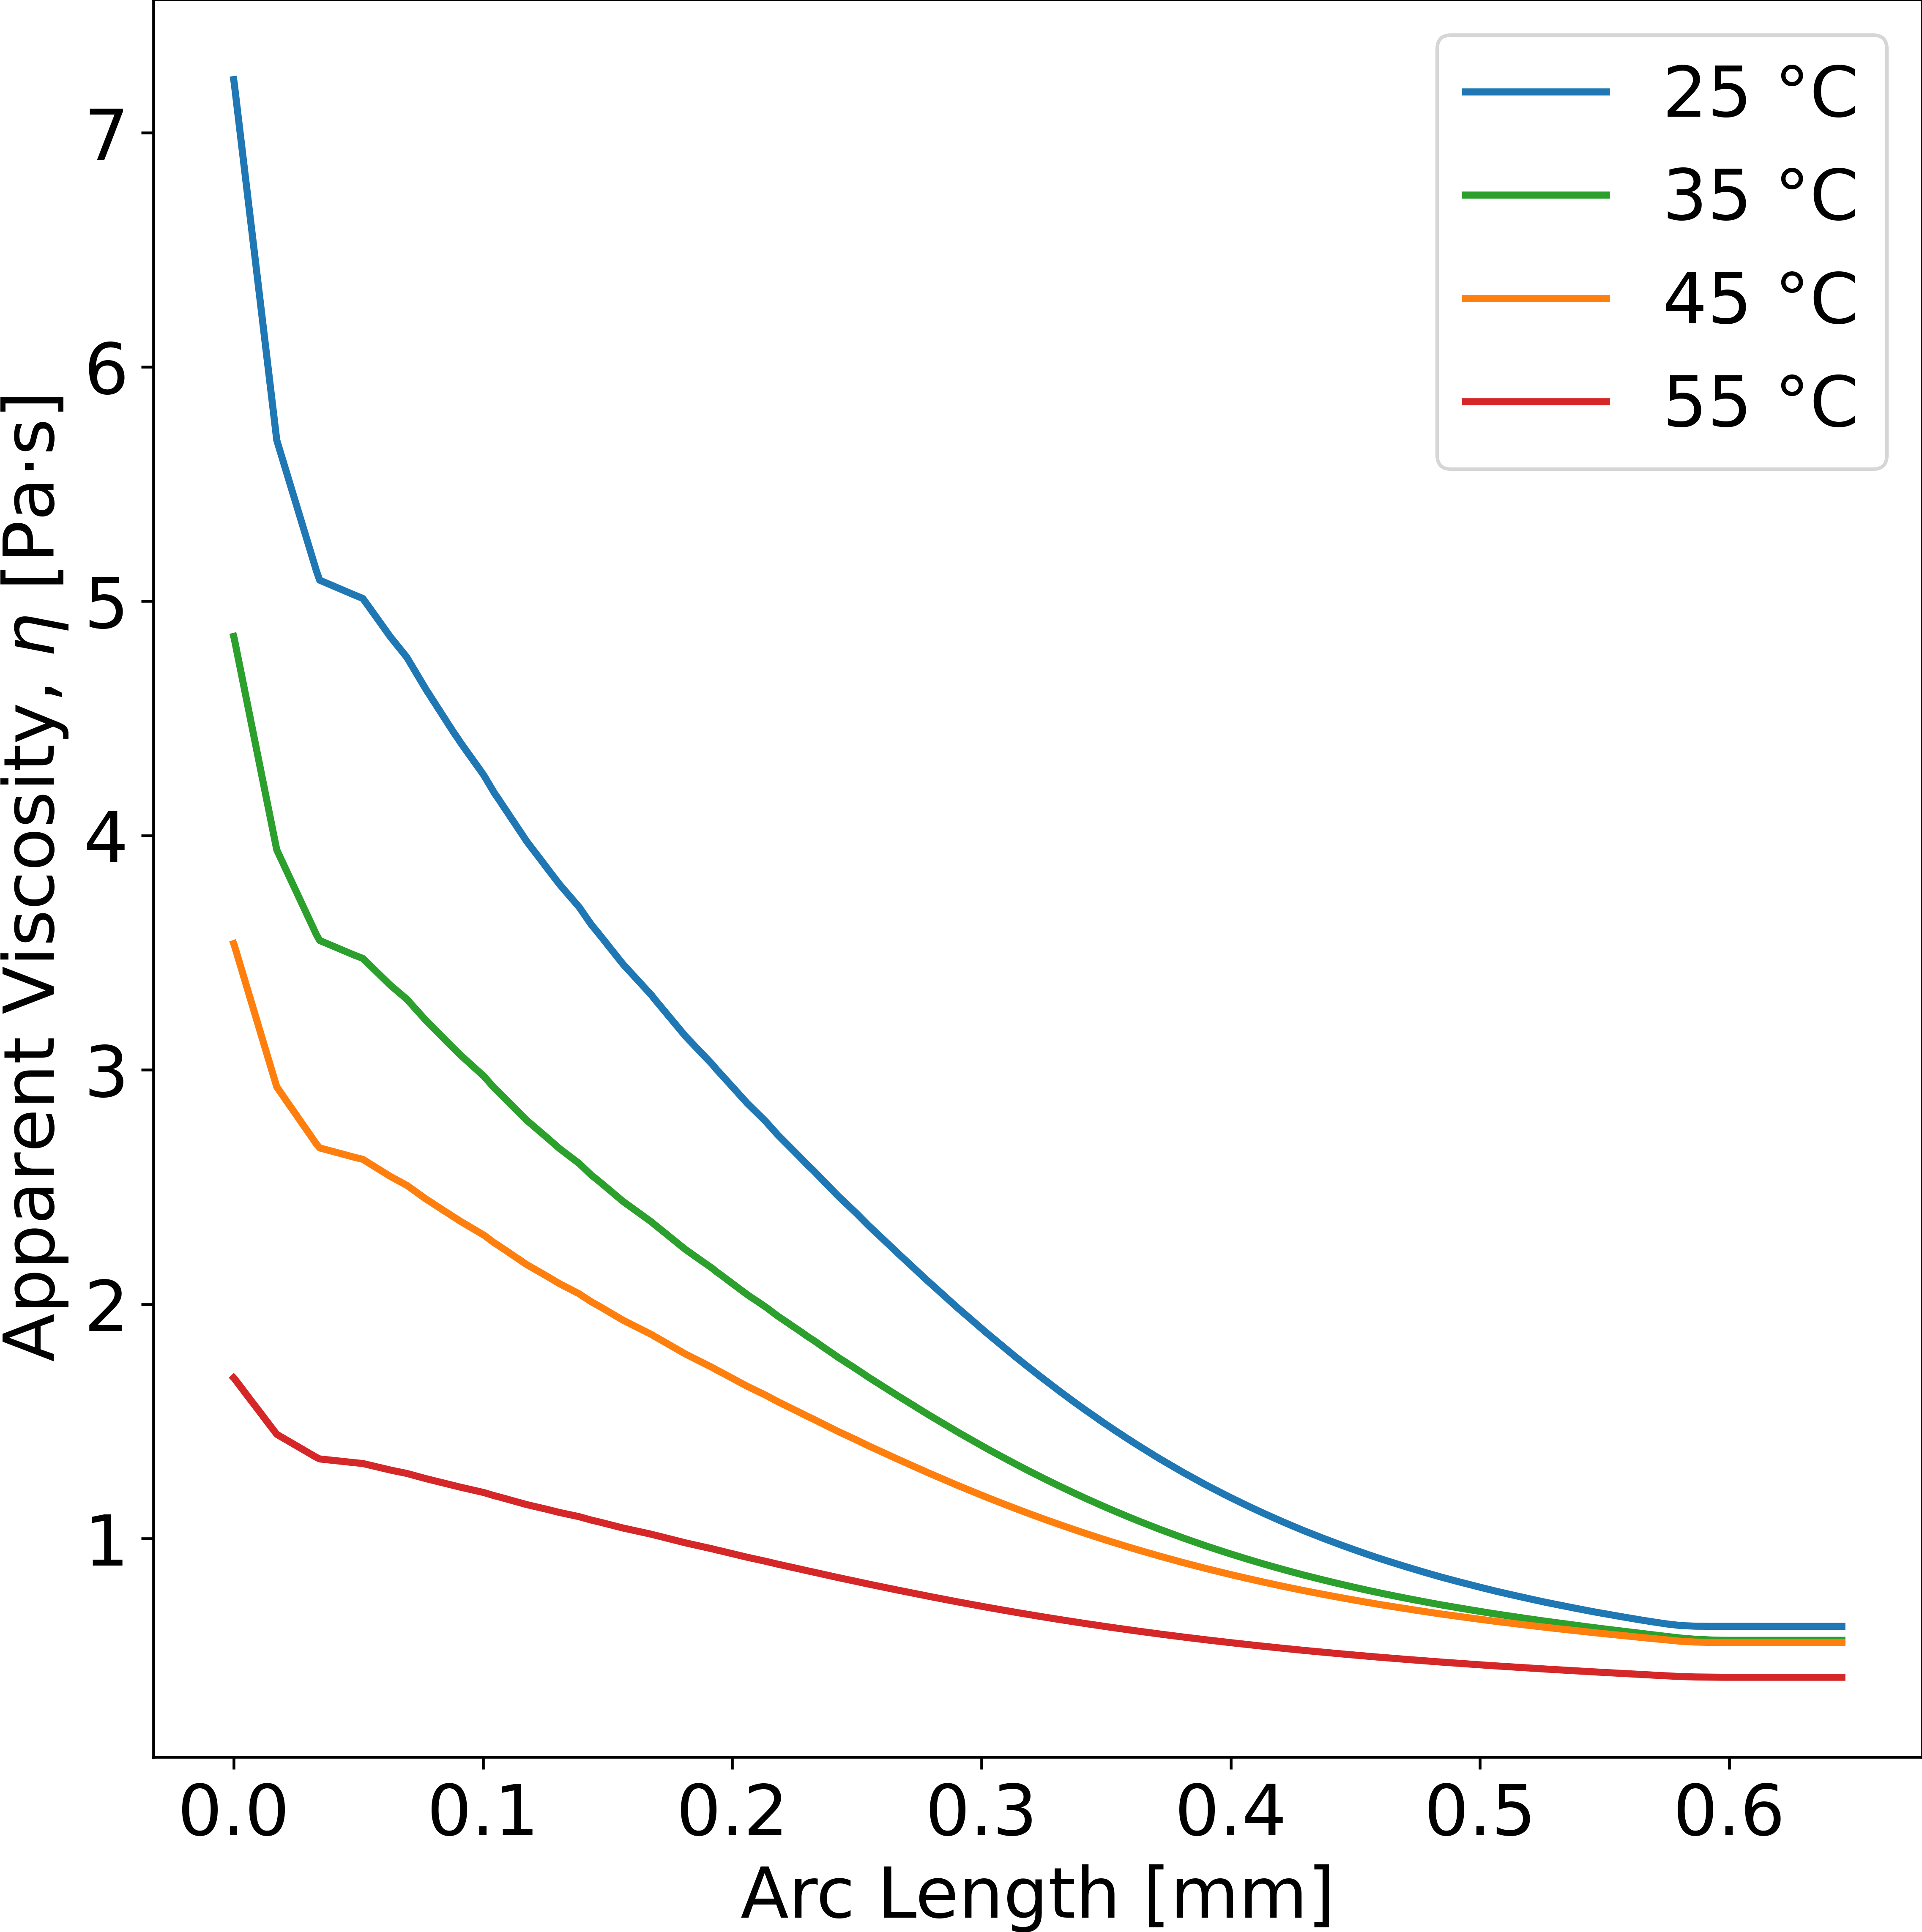
\includegraphics[trim = 0mm 0mm 0mm 0mm, clip, width=1.9in]{./images/tapered_nudata_sphere.png}
\end{column}
\end{columns}

{\let\thefootnote\relax\footnote{{Arc length: the circle’s circumference cut by the sphere near the needle inlet for cylindrical needles, and the needle outlet for the tapered needle; see Appendix I.}}}
\end{frame}


% 11 ---------------------------
\begin{frame}{Stresses under the influence of Temperature Changes}

\footnotesize
\begin{itemize}
    \item As temperature $\Uparrow$, stresses near the needle inlet $\Downarrow$. Stresses experience little change when the temperature changes from 35 $^{\circ}$C to 45 $^{\circ}$C, indicating a nonlinear relationship.
\end{itemize}
\vspace{-3.5mm}
\begin{columns}
\begin{column}{.333\textwidth}
\begin{itemize}
    \item 90$^{\circ}$ cylindrical needle:
\end{itemize}
\vspace{0.5mm}
\centering
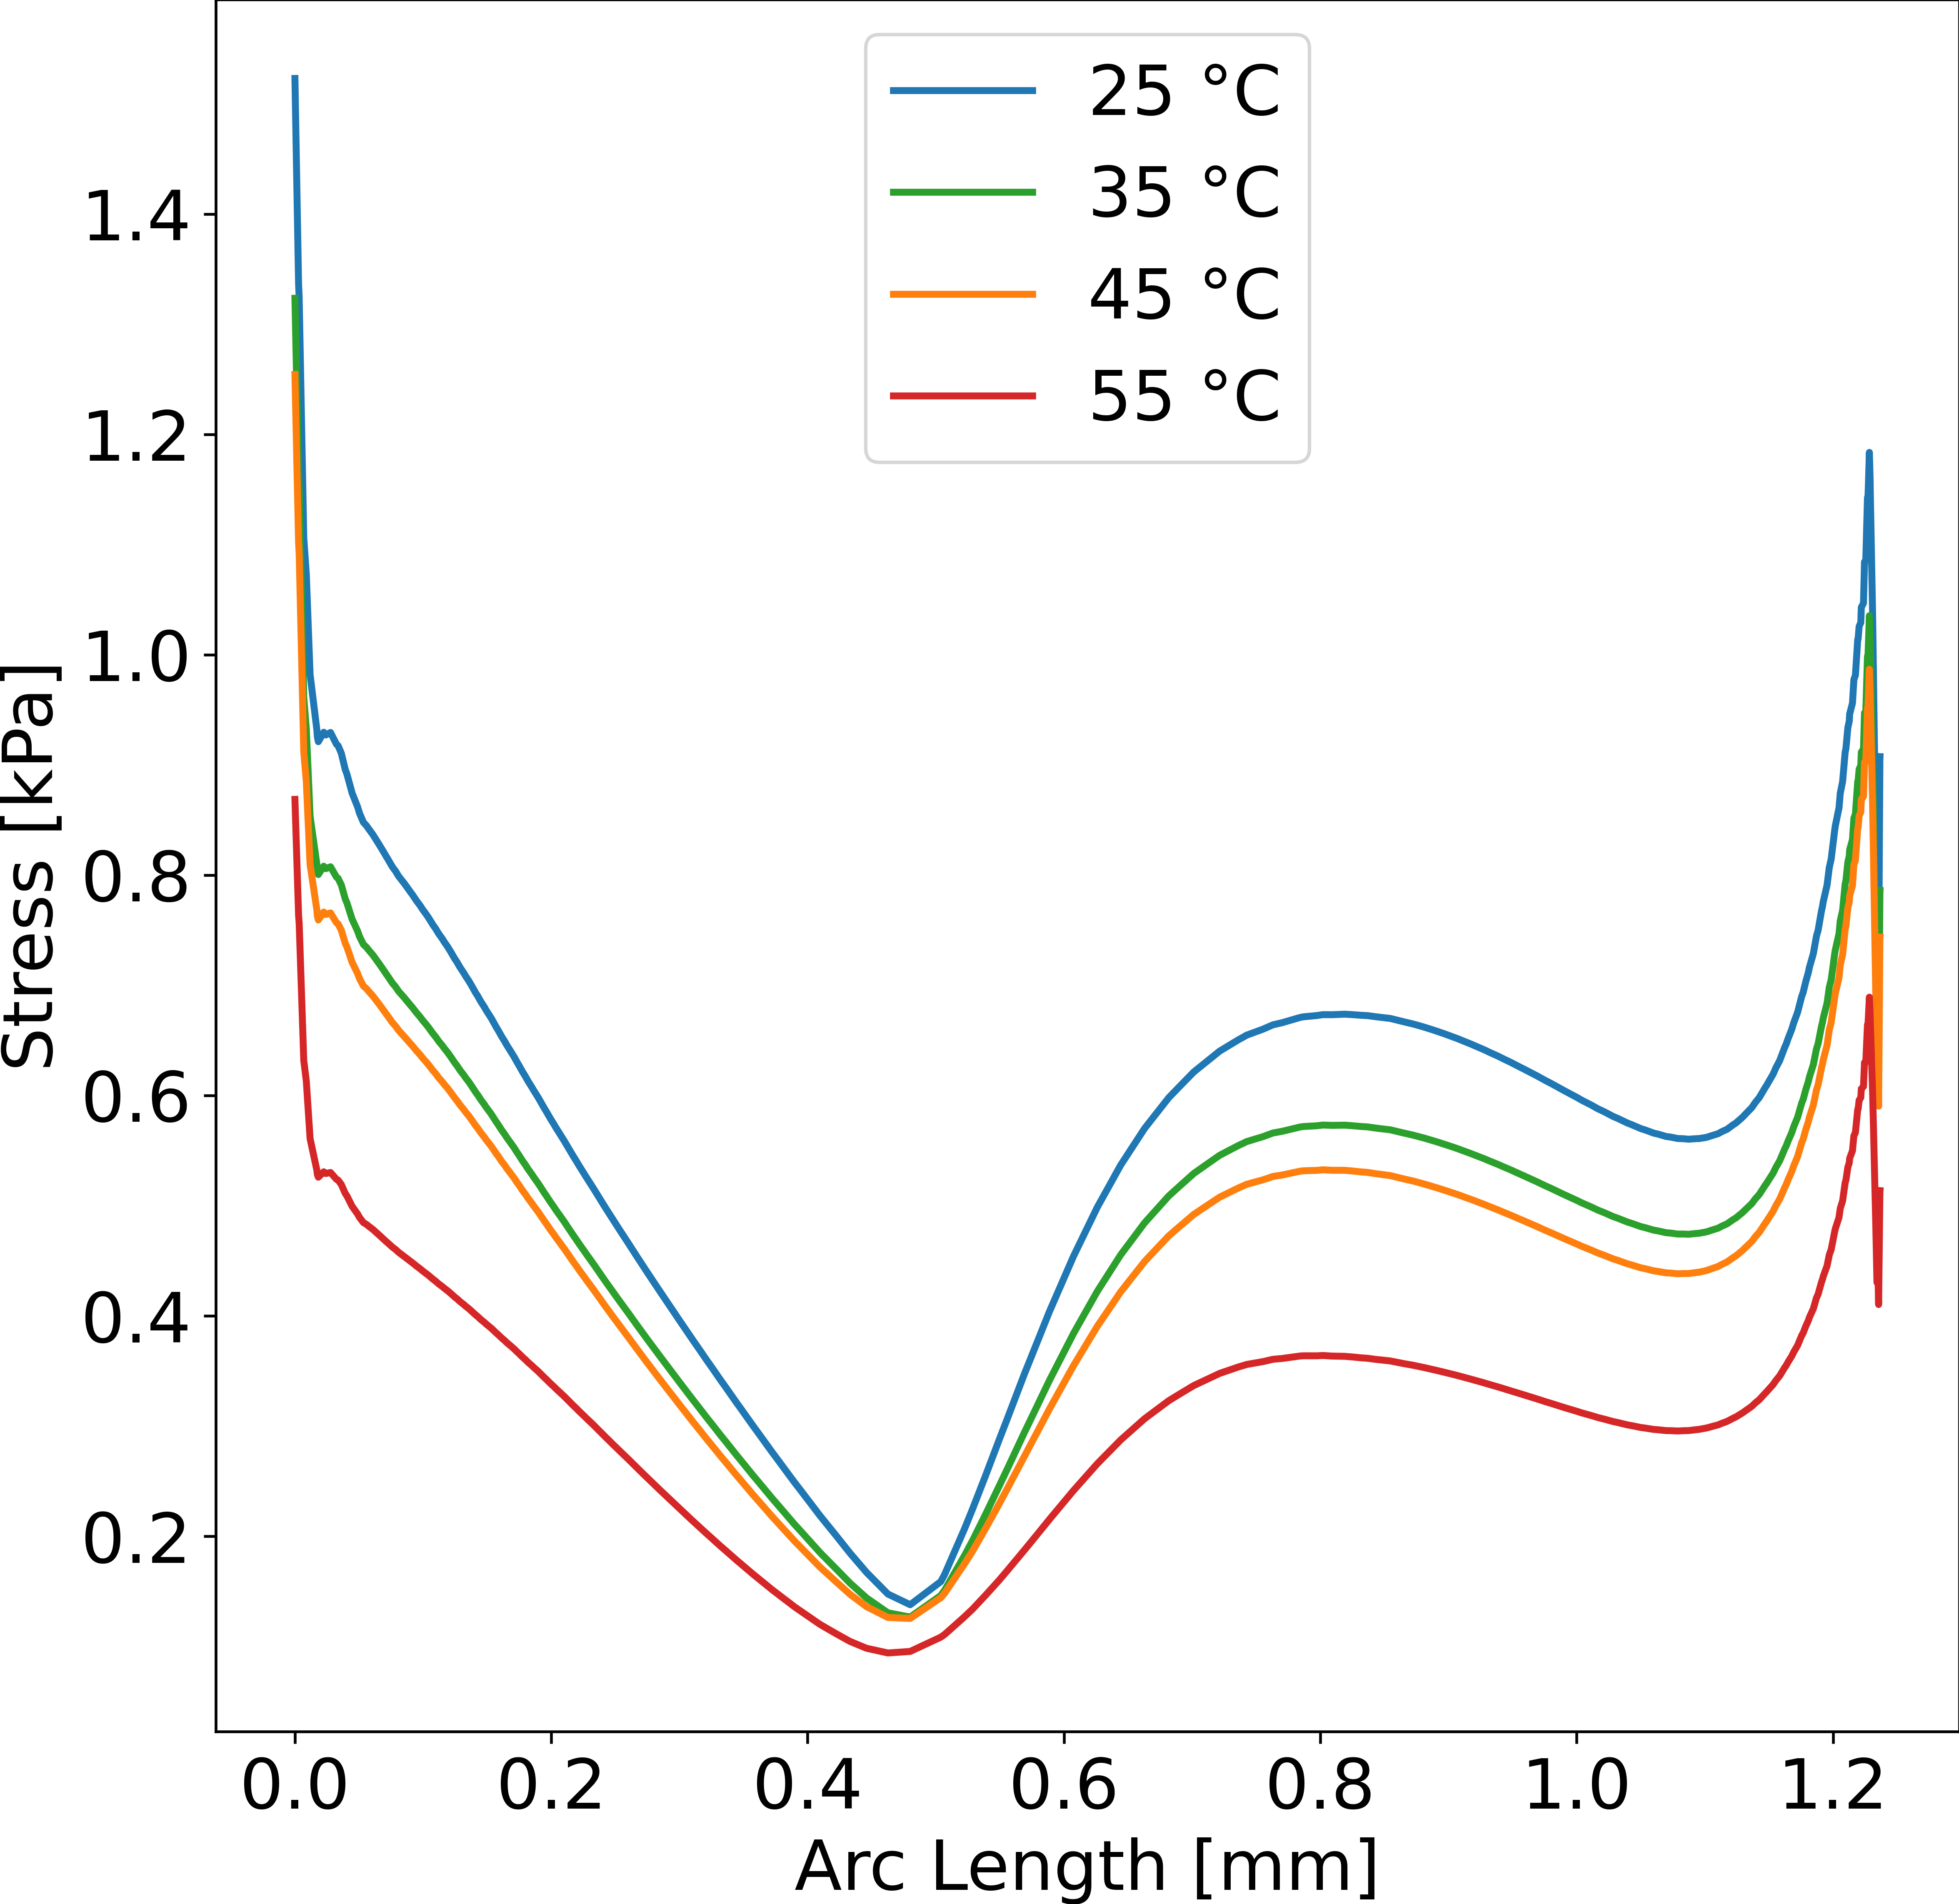
\includegraphics[trim = 0mm 0mm 0mm 0mm, clip, width=1.95in]{./images/90_ssdata_sphere.png}
\end{column}

\begin{column}{.333\textwidth}
\begin{itemize}
    \item 45$^{\circ}$ cylindrical needle:
\end{itemize}
\vspace{0.5mm}
\centering
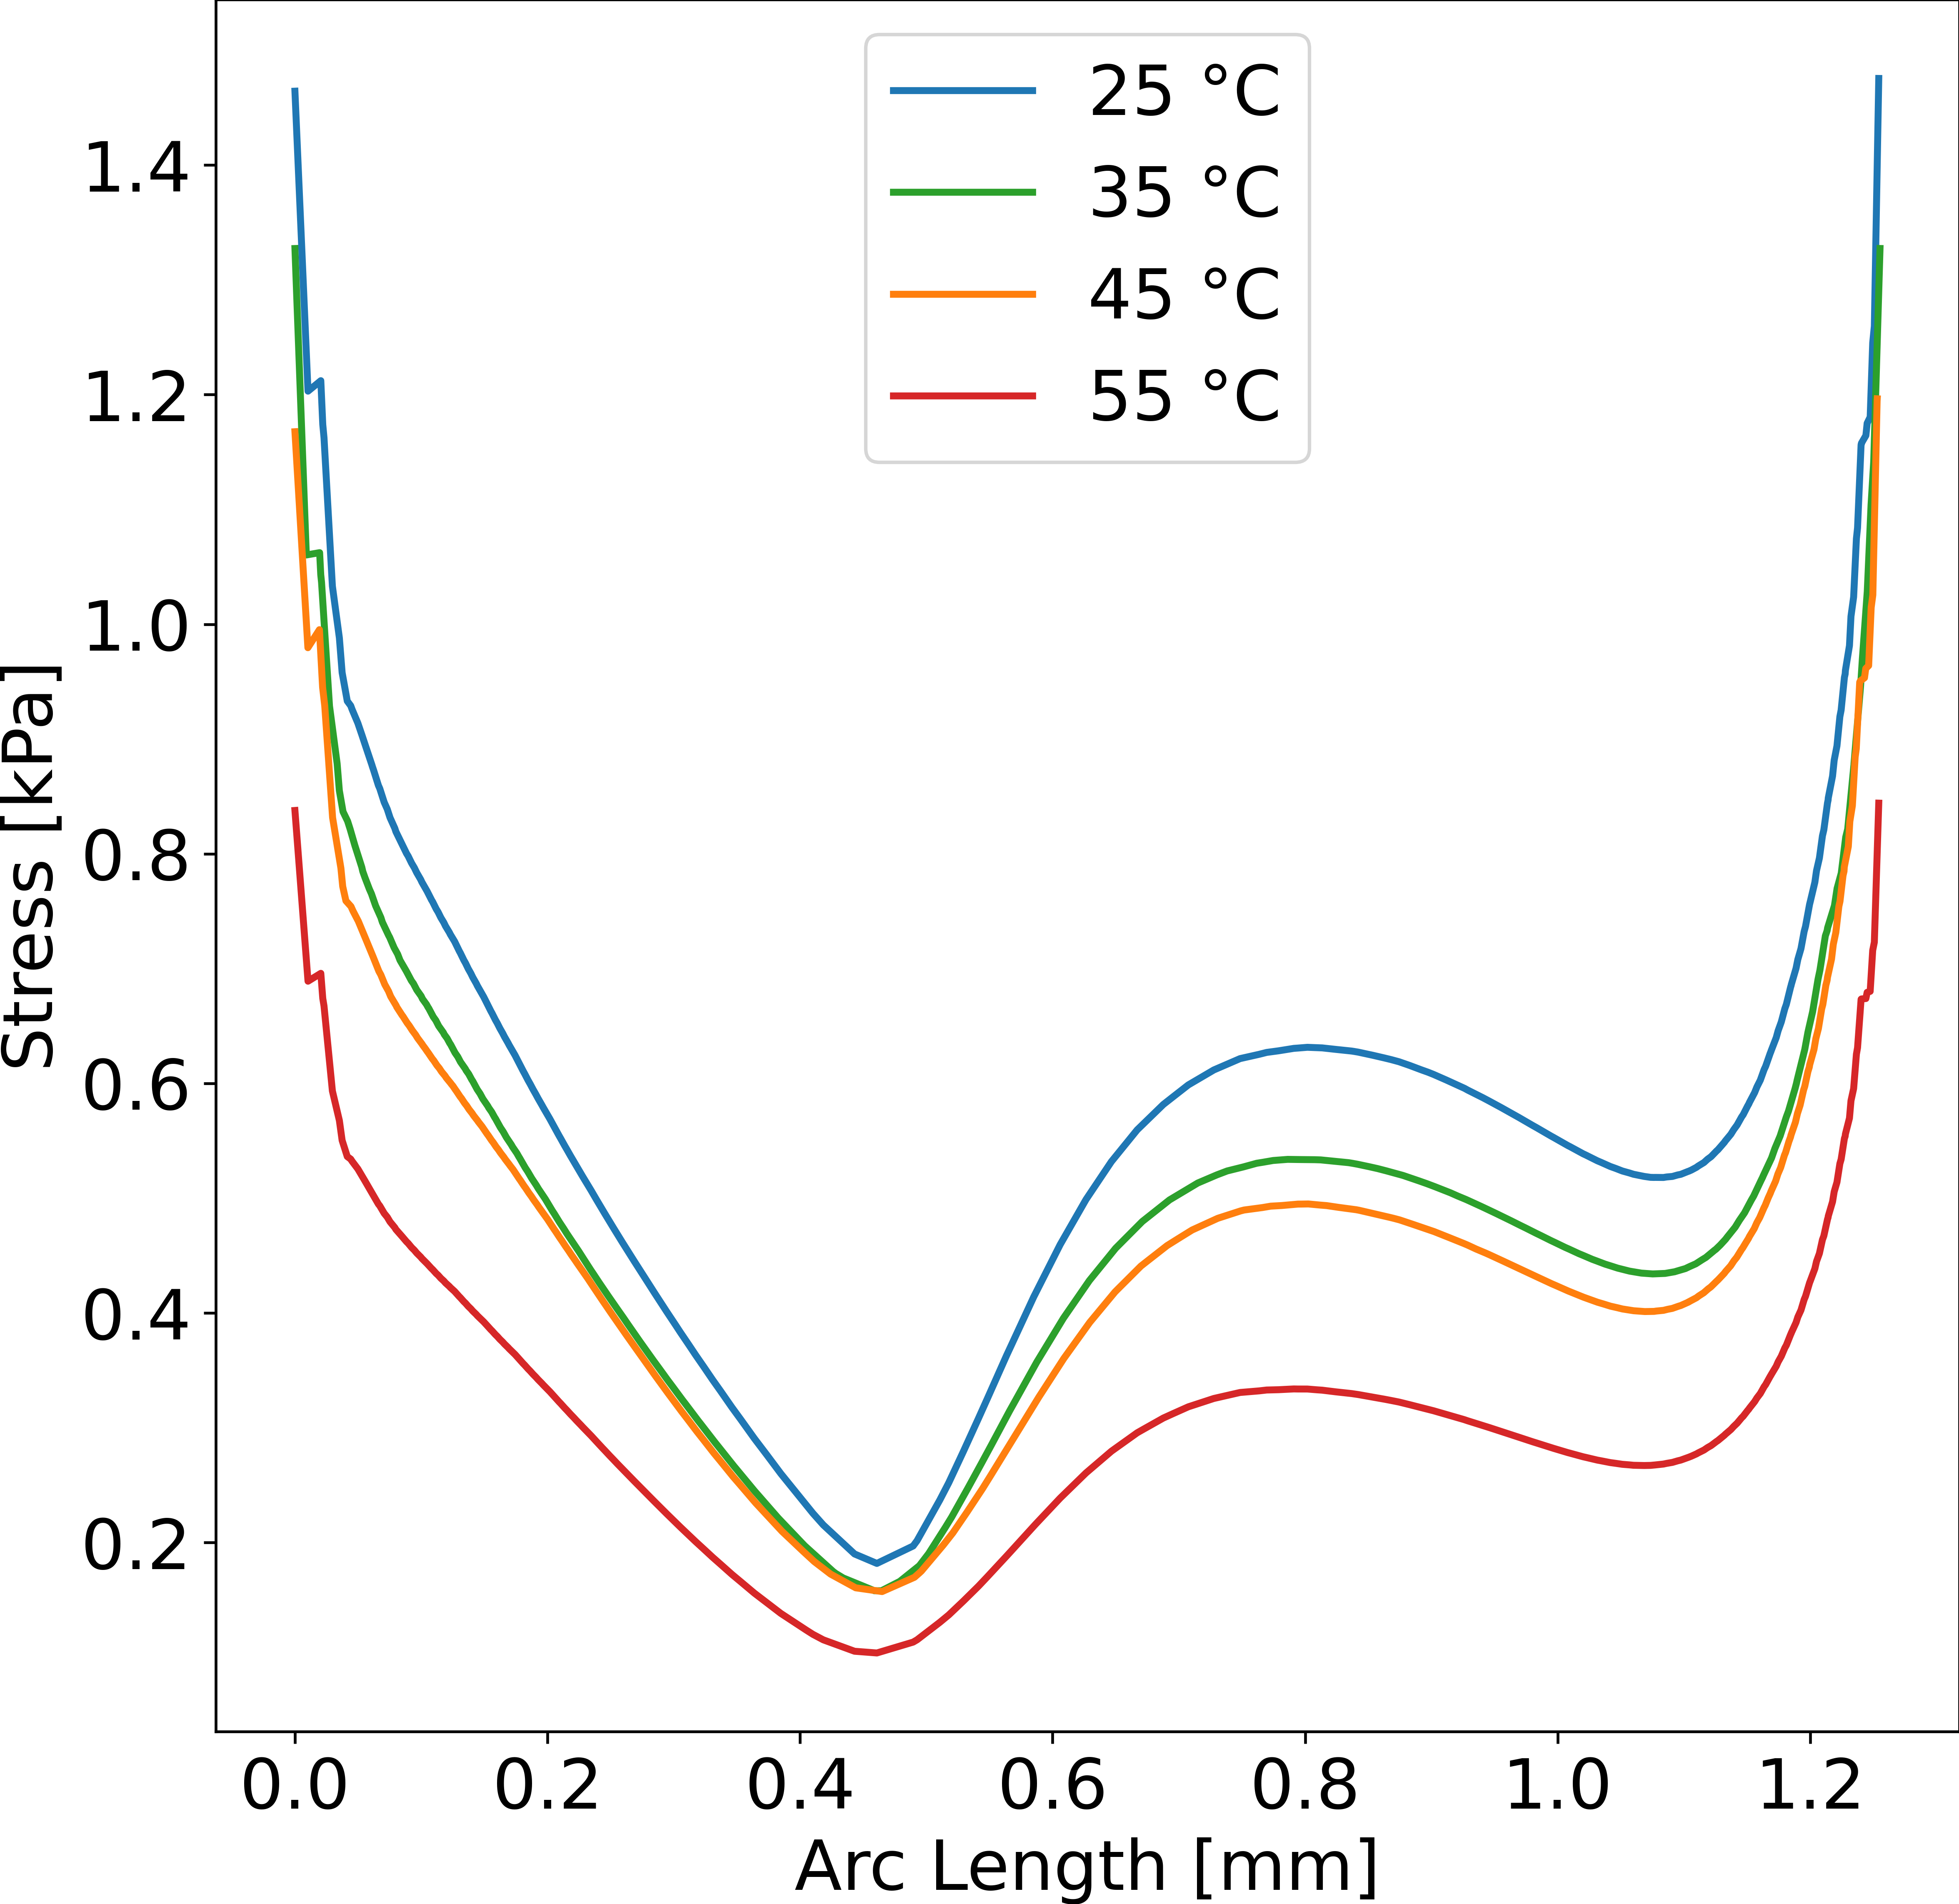
\includegraphics[trim = 0mm 0mm 0mm 0mm, clip, width=1.95in]{./images/45_ssdata_sphere.png}
\end{column}

\begin{column}{.333\textwidth}
\begin{itemize}
    \item Tapered needle:
\end{itemize}
\vspace{0.5mm}
\centering
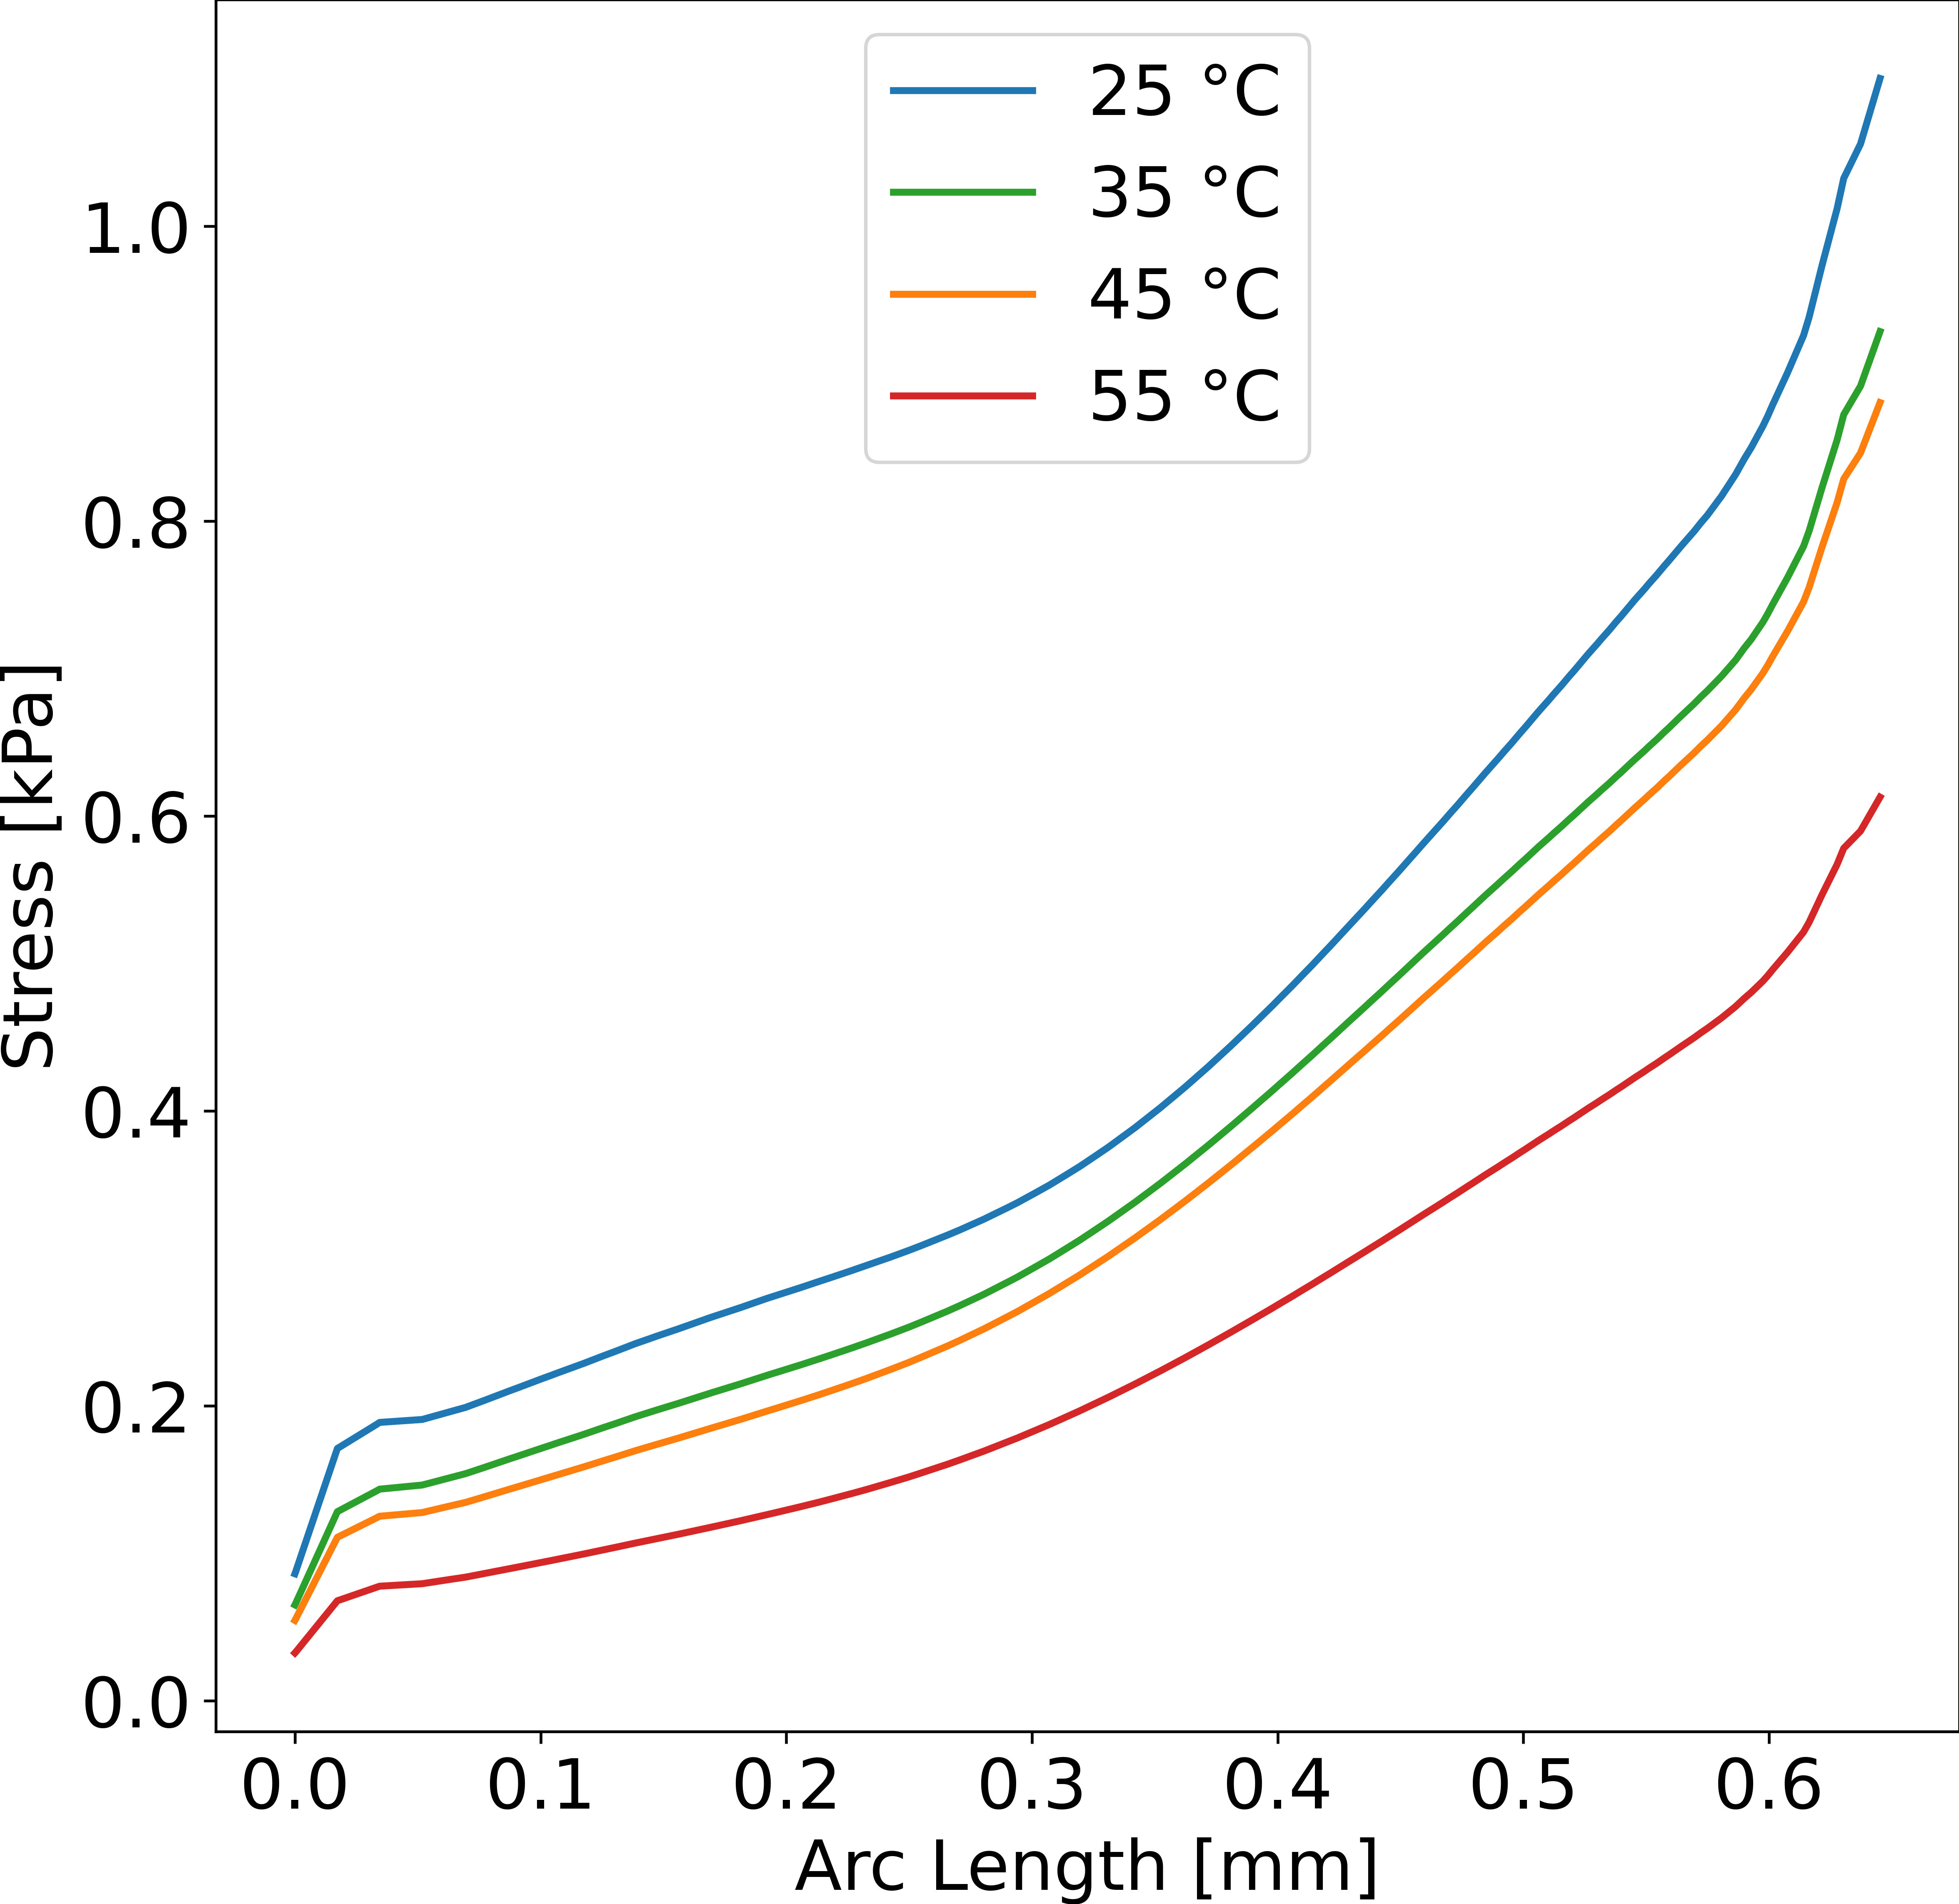
\includegraphics[trim = 0mm 0mm 0mm 0mm, clip, width=1.95in]{./images/tapered_ssdata_sphere.png}
\end{column}
\end{columns}

\end{frame}

% 12 ---------------------------
\begin{frame}{The Herschel–Bulkley Fluid Model$^{\text{5,6}}$}
\small
\begin{columns}
\column{.65\textwidth}
\vspace{-4mm}
\begin{itemize}
    \item Herschel–Bulkley fluid: $\tau = \tau_0 + K\dot{\gamma}^{n}$
    \item Nonlinear regression of experimental rheological data, where $T_0, T_1, T_2, C_0, C_1, C_2, a, b, d, f, g, h, i, j,$ and $m$ are constants (alginate-based bioinks):
\end{itemize}
\vspace{-1mm}
\centering
\begin{equation*}
    K = a \exp{(\frac{T_0}{T}-\frac{C_0}{C})}-b(\frac{T}{T_0}\frac{C}{C_0})+d(\frac{T_0}{T})
\end{equation*}
\begin{equation*}
    \tau_0 = f \exp{(\frac{T_1}{T}-\frac{C}{C_1})}+g(\frac{T_1}{T}\frac{C}{C_1})^{T/T_1}+h(\frac{T_1}{T})
\end{equation*}
\begin{equation*}
    n = i \exp{(-\frac{T_2}{T}-\frac{C_2}{C})}-j(\frac{T_2}{T}\frac{C_2}{C})+m(\frac{T}{T_2})
\end{equation*}
\begin{equation*}
    \boxed{25\ ^{\circ}\text{C}\leq T \leq 55\ ^{\circ}\text{C}; 1\%\ \text{(w/v)}\leq C \leq 4\%\ \text{(w/v)}}
\end{equation*}

\column{.35\textwidth}
\centering
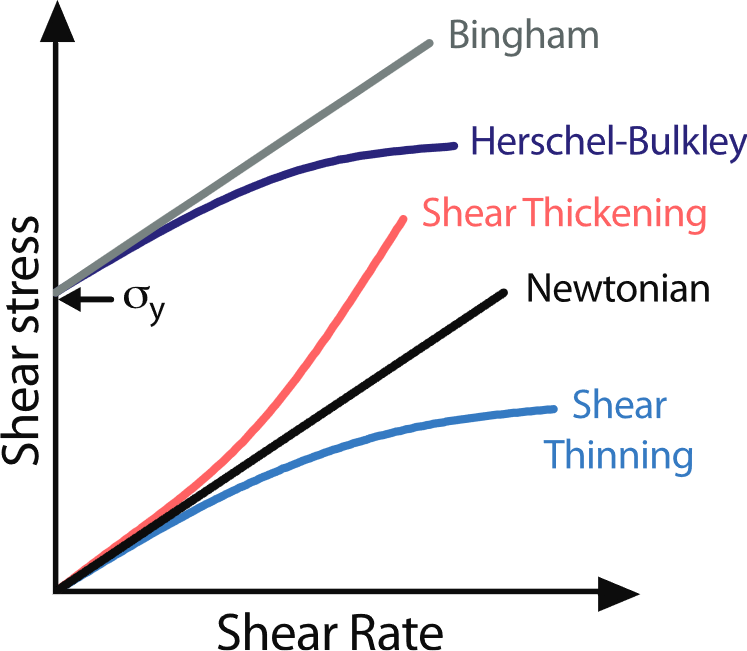
\includegraphics[trim = 0mm 0mm 0mm 0mm, clip, width=1.65in]{./images/fluid_type.png}
\begin{table}
\begin{tabular}{ c | c }
Symbol & Description \\
\hline \hline
$\tau$ & Shear stress\\
$\tau_0$ or $\sigma_y$ & Yield stress\\
$T$ & Temperature\\% in Celsius\\
$C$ & Mass concentration% in \% (w/v)
\end{tabular}
%\caption{}
\end{table}
\end{columns}

\addtocounter{footnote}{-1}
\stepcounter{footnote}\footnotetext{\cite{cooke_rheology_2021}}

\end{frame}

% 13 ---------------------------
\begin{frame}{Additional Governing Equations}
\begin{itemize}
\item $\nabla \cdot \boldsymbol{V} = 0$ \hfill(Incompressible continuity equation)
\end{itemize}

\begin{itemize}
\item $\rho \frac{\partial \boldsymbol{V}}{\partial t} + \rho \boldsymbol{V} \cdot \nabla\boldsymbol{V} -\nabla \cdot (\eta \nabla \boldsymbol{V}) = -\nabla P + \boldsymbol{F_{\sigma}} + \rho \boldsymbol{g}$ \hfill(Navier–Stokes equations)
\end{itemize}

\begin{itemize}
\item $\frac{\partial \alpha}{\partial t} + \boldsymbol{V} \cdot \nabla \alpha + \nabla \cdot [(\boldsymbol{V_1} - \boldsymbol{V_2})\alpha (1-\alpha)] = 0$ \hfill(Volume fraction equation)
\end{itemize}

\begin{itemize}
\item $\eta = \text{min}(\eta_0, \tau_0/\dot{\gamma}+K\dot{\gamma}^{n-1})$ \hfill(Herschel–Bulkley fluid model)
\end{itemize}
\vspace{4mm}
\begin{columns}
\column{.5\textwidth}
\begin{block}{}
\vspace{-5mm}
\begin{align*}
\boldsymbol{V} &= \alpha\boldsymbol{V_1} + (1-\alpha)\boldsymbol{V_2}\\
\rho &= \alpha\rho_1 + (1-\alpha)\rho_2\\
\eta &= \alpha\eta_1 + (1-\alpha)\eta_2\\
\boldsymbol{F_{\sigma}} &= \sigma \kappa \nabla \alpha\\
\kappa &= -\nabla \cdot ({\nabla\alpha}/{|\nabla\alpha|})
\end{align*}
\end{block}

\column{.5\textwidth}
\centering
\scalebox{0.8}{
\begin{tabular}{ c | c }
Symbol & Description \\
\hline \hline
$\boldsymbol{V}$ & Velocity vector of both phases (1 \& 2)\\
$t$ & Time\\
$\boldsymbol{F_{\sigma}}$ & Continuum surface force\\
$\sigma$ & Surface tension\\
$\kappa$ & Mean curvature of the free surface\\
$\alpha$ & Phase fraction ($0 \leq \alpha \leq 1$)\\
$\boldsymbol{g}$ & Gravitational acceleration\\
$\eta_0$ & Viscosity at low shear rate
\end{tabular}
}

\end{columns}
\end{frame}

% 14 ---------------------------
\begin{frame}{Assessment of Printability}

\begin{columns}
\column{.66\textwidth}
\begin{itemize}
    \item Extrudability, filament formation, and shape fidelity, indicating the degree of dimensional faithfulness of the printed object vs. computer-aided design (CAD).\footnotemark
    \item Model Validation
    \begin{itemize}
        \item The diameter of the printed strand is given by:
    \end{itemize}
\end{itemize}
\begin{columns}
\column{.55\textwidth}
\[
\tikzmarknode{A}{D} = \sqrt{\frac{4\tikzmarknode{C}{Q}}{\pi \tikzmarknode{B}{V_m}}}
\begin{tikzpicture}[overlay, remember picture,shorten <=1mm,
                    nodes={inner sep=1pt, align=center, font=\tiny},
                    every path/.style = {draw=black, Stealth-}] % <---
\draw (A.south) -- ++ (-.3,-.5) node[below] {Strand\\diameter};
\draw (B.south) -- ++ (.3,-.5) node[below] {Horizontal needle\\moving speed};
\draw (C.east) -- ++ (1,-.3) node[below] {Volumetric\\flow rate};
\end{tikzpicture}
\vspace{0.85cm}
\]
\column{.45\textwidth}
\begin{block}{Assumptions:}
\begin{enumerate}[I]\setlength{\itemsep}{0.01mm}
\setbeamertemplate{enumerate items}[square]
    \item Perfect cylindrical strand
    \item No spreading (2D)
\end{enumerate}
\end{block}
\end{columns}
\begin{itemize}
    \item Herschel–Bulkley Fluid Model 
    \begin{itemize}
    \scriptsize
        \item $K = 29.86$ Pa$\cdot \text{s}^\text{n}$, $n = 0.46$, $\tau_0 = 33.82$ Pa
        \item $T$ = 25 $^{\circ}\text{C}$, $C$ = 2.5\% (w/v)
        \item $R$ = 400 $\mu$m, $Q$ = 50 $\mu$L/s, $V_{m}$ = 5 mm/s
        \item $D$ $\approx$ 3.57 mm, $D_\text{simulation} \approx$ 2.90 mm (81.1\%)
    \end{itemize}
\end{itemize}

\column{.34\textwidth}
\centering

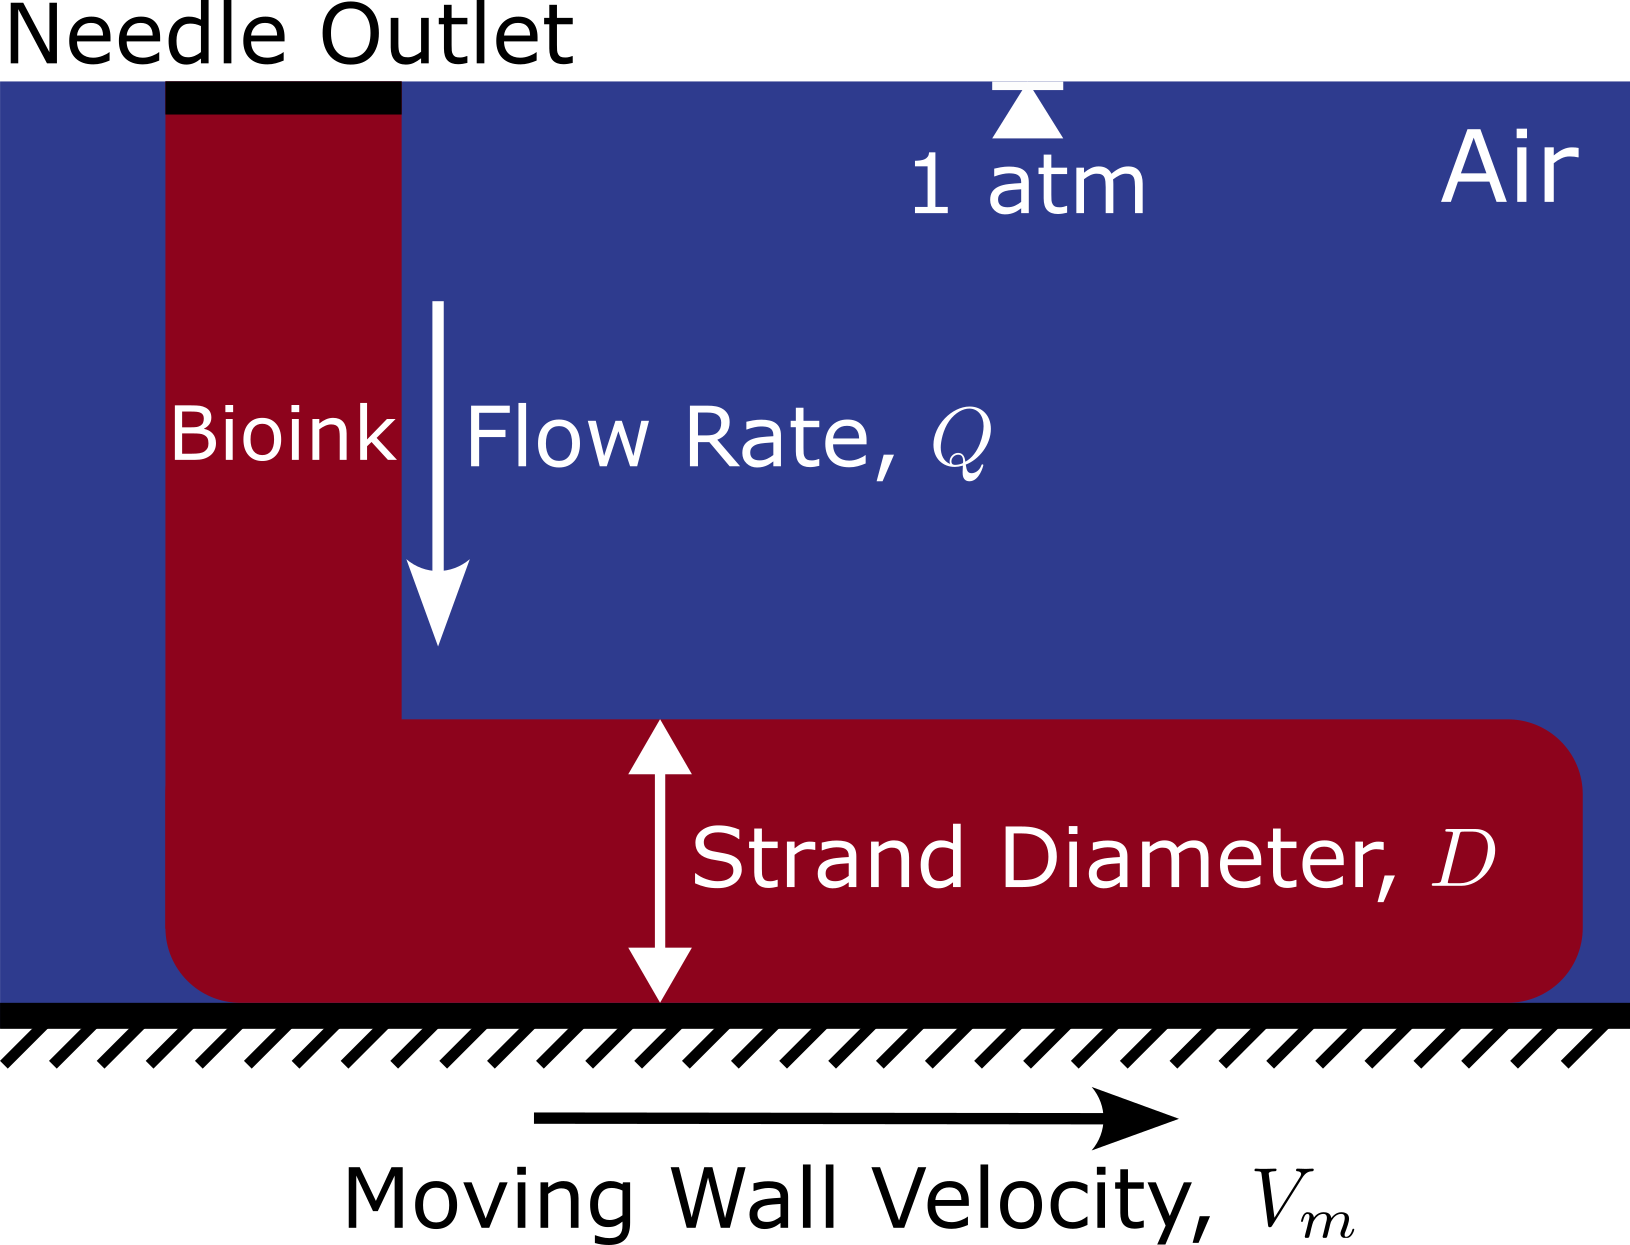
\includegraphics[trim = 0mm 0mm 0mm 0mm, clip, width=1.70in]{images/printability_setup.png}\\
%\includegraphics[trim = 0mm 0mm 0mm 0mm, clip, width=1.65in]{example-image-b}
\animategraphics[width=1.55in, autoplay, controls, loop]{15}{animations/anime.}{0000}{0100}
\end{columns}
\addtocounter{footnote}{-1}
\stepcounter{footnote}\footnotetext{\cite{schwab_printability_2020}}
\end{frame}

% 15 ---------------------------
\begin{frame}{Assessment of Cell Viability}%$^{\text{7}}$}
\begin{itemize}
    \item Existing model ($R^2$ of 0.859; error of 9.2\%; human fibroblast; size $\sim 30 \mu$m)\footnotemark:
    \begin{itemize}
        \item \fbox{$V_{\text{fibroblast}}(\tau_w, t_r, \eta) = 145.753-0.0133752*\tau_w-0.405308*t_r+0.00642919*\eta$}\vspace{1mm}
        \item $t_{\text{r, simulation}} = L_n / \bar{U} \approx$ 130 ms
    \end{itemize}
\end{itemize}
\vspace{-3mm}
\begin{columns}
\column{.5\textwidth}
\centering
\begin{table}
\begin{tabular}{ c | c }
Symbol & Description \\
\hline \hline
$V$ & Viable cells ratio (\%)\\
$\tau_w$ & Wall shear stress (Pa)\\
$t_r$ & Residence time (ms)\\
$\eta$ & Apparent viscosity (Pa$\cdot$s)
\end{tabular}
%\caption{}
\end{table}
\column{.5\textwidth}
\centering
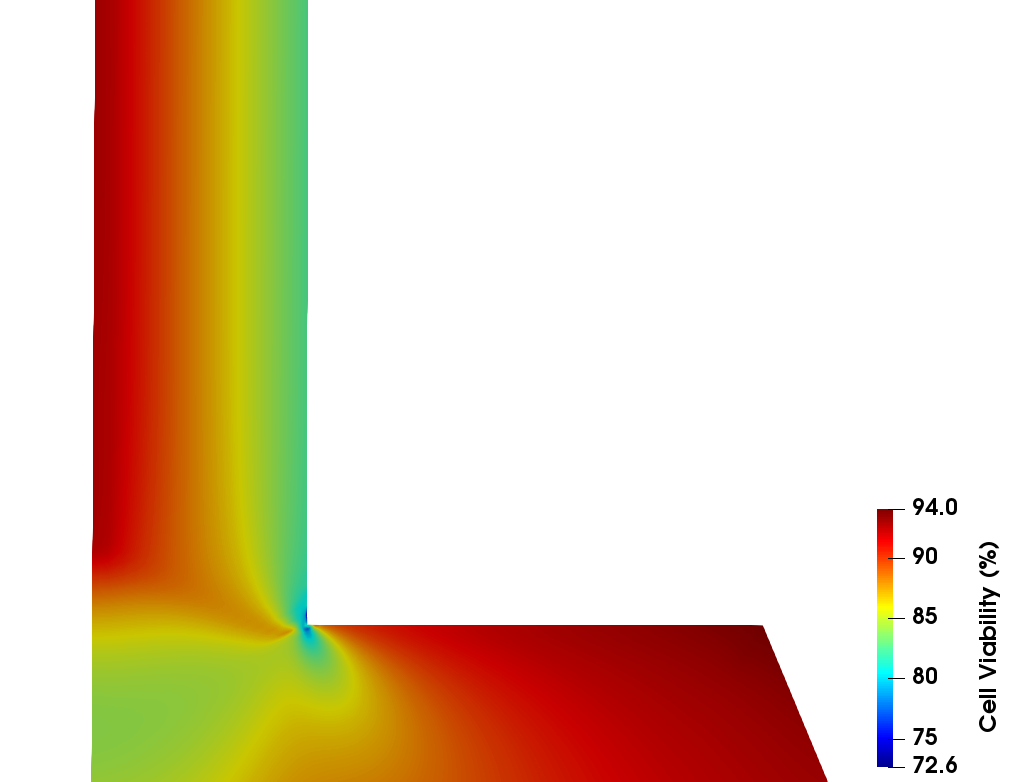
\includegraphics[trim = 0mm 0mm 0mm 0mm, clip, width=1.95in]{images/cell_viability_90_25C.png}
\end{columns}
\vspace{-3mm}
\begin{itemize}
    \item Cell types and shear stress\footnotemark
    \begin{itemize}
        \item 5000 Pa $\rightarrow$ fibroblasts’ viability drop below 80\% over 30 ms.
        \item 160 Pa $\rightarrow$ detrimental to chondrocyte's viability.
        \end{itemize}
\end{itemize}
\addtocounter{footnote}{-2}
\stepcounter{footnote}\footnotetext{\cite{lemarie_rheology_2021}}
\stepcounter{footnote}\footnotetext{\cite{webb_parameter_2017}}

\end{frame}

% 16 ---------------------------
\begin{frame}{Conclusion}
\begin{block}{}
\begin{itemize}
\item The tapered nozzle exhibits the least stresses in both magnitude and area; however, when printing in a support bath, tapered nozzles are not suitable.
\item Extensional stress at the needle inlet region has the most detrimental effect on cells.
\item The 90$^{\circ}$ cylindrical needle provides a smaller maximum wall stress area, but a higher extensional stress region at the needle inlet region over its 45$^{\circ}$ counterpart.
\item Using preheated bioink results in a significant reduction in stresses during extrusion.
\item Herschel–Bulkley fluid model provides an estimate (81.1$\%$) on printed strand diameter.
\item Among the 3 main factors (shear stress, residence time, and apparent viscosity) that influence cell viability, shear stress exhibits the most significant impact; shear stress distribution and cell viability are closely related.
\end{itemize}
\end{block}

\end{frame}

% 17 ---------------------------
\begin{frame}{Future Works}
\begin{block}{}
\begin{itemize}
    \item Investigating the magnitude of stresses of the printed strand at various moving wall velocities.
    \item Determining how concentrations of alginate-based bioinks affect the magnitude of stresses.
    \item Optimizing the printing/extrusion speed, environmental temperature, gelation, and cell viability for various types of bioinks and needle geometries.
    \item Utilizing machine learning to estimate cell viability.
    
    %\item Performing Lagrangian particle tracking simulation to determine cell concentration within the needle with different volumetric flow rates.
    
\end{itemize}
\end{block}

\begin{columns}
\column{.333\textwidth}
\centering

\includegraphics[trim = 0mm 0mm 0mm 0mm, clip, width=1.8in]{./images/DL.png}
\\\tiny Copyright {\fontfamily{cmr}\selectfont\textcopyright}\ 2021. No Starch Press, Inc.\\Illustrator: Gina Redman

\column{.333\textwidth}
\centering
\scalebox{0.7}{
\begin{tabular}{ c | c}
Input, $x_n$ & Output, $y_k$\\
\hline \hline
Consistency index & \\
Flow index \\
Concentration & \\
Bioink's temperature & Cell viability\\
Volumetric flow rate & \\
Needle radius & \\
Needle length & 
\end{tabular}
}

\column{.333\textwidth}
\centering
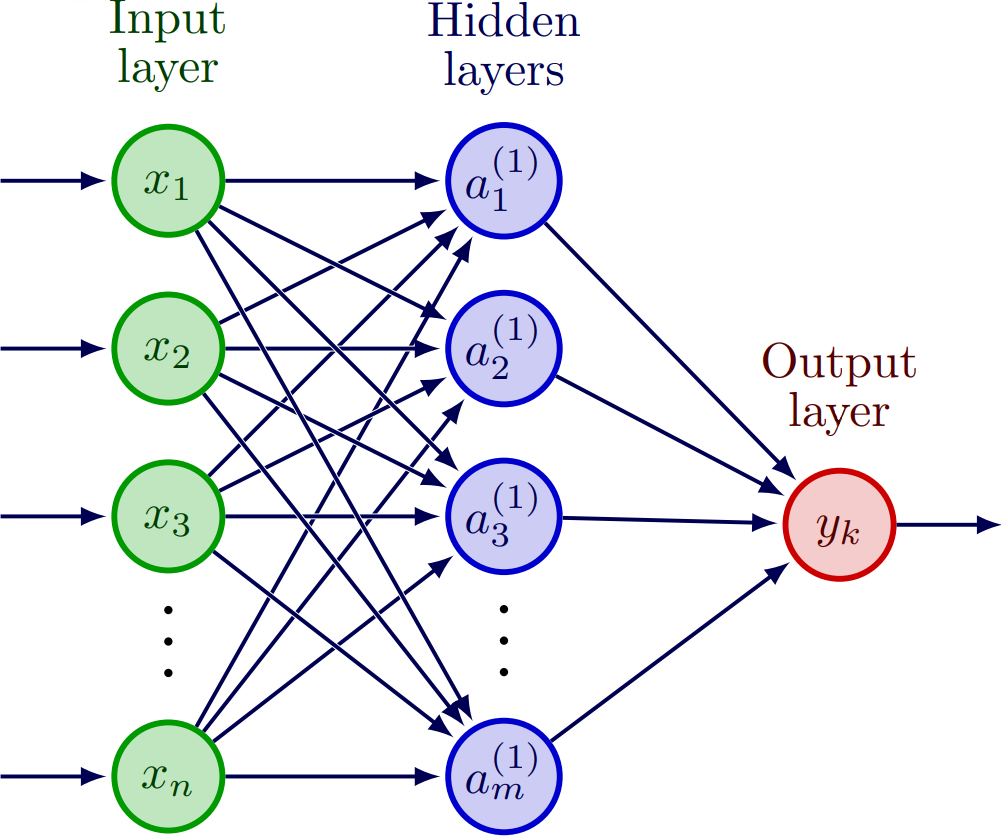
\includegraphics[trim = 0mm 0mm 0mm 0mm, clip, width=1.8in]{./images/NN.png}
\end{columns}
\end{frame}

% 18 --------------------------- (References)
\AtNextBibliography{\scriptsize}
\begin{frame}[plain,noframenumbering]%[t,allowframebreaks]
    \settoggle{bbx:url}{false}
    \settoggle{bbx:doi}{false}
    \settoggle{bbx:eprint}{false}
    \frametitle{References}
    \printbibliography
\end{frame}


%\iffalse



% Appendix I ---------------------------
\begin{frame}[plain,noframenumbering]{Appendix I}
\begin{itemize}
    \item Arc length definition:
    \begin{itemize}
        \item Plotting the circle's circumference cut by the sphere, rotating \textbf{counterclockwise}.
        \item Sphere center: (0, 0.2 mm, 7.48 mm), *tapered needle: (0, 0.2 mm, 20.48 mm)
        \item Sphere radius: 0.2 mm
        \item Starting point: (0, 0.4 mm, 7.48 mm), *tapered needle: (0, 0.4 mm, 20.48 mm)
    \end{itemize}
\end{itemize}
\vspace{1mm}
\centering
\includegraphics[trim = 0mm 0mm 0mm 0mm, clip, width=2.1in]{./images/arc_length.png}
\end{frame}


% Appendix II ---------------------------
\begin{frame}[plain,noframenumbering]{Appendix II}
\begin{itemize}
    \item Velocity vector fields colored by the magnitude of stresses (kPa) for various needle types at 25 $^{\circ}$C:
\end{itemize}
\vspace{3mm}
\centering
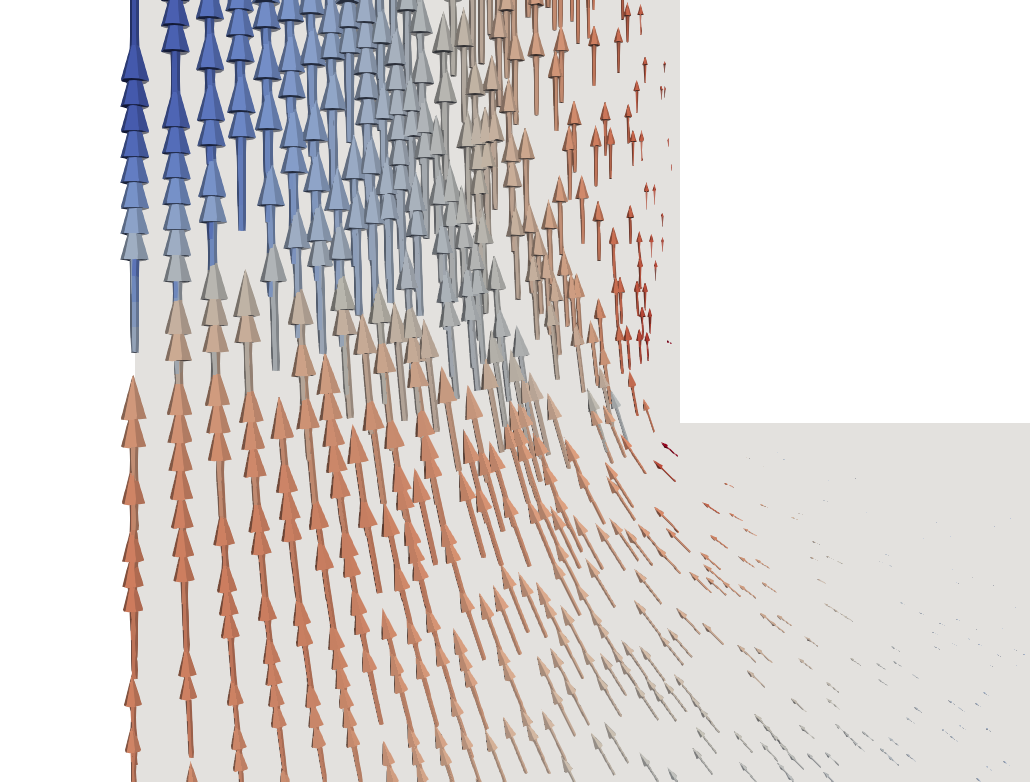
\includegraphics[trim = 0mm 0mm 0mm 0mm, clip, width=1.955in]{./images/90_stress_vector.png}
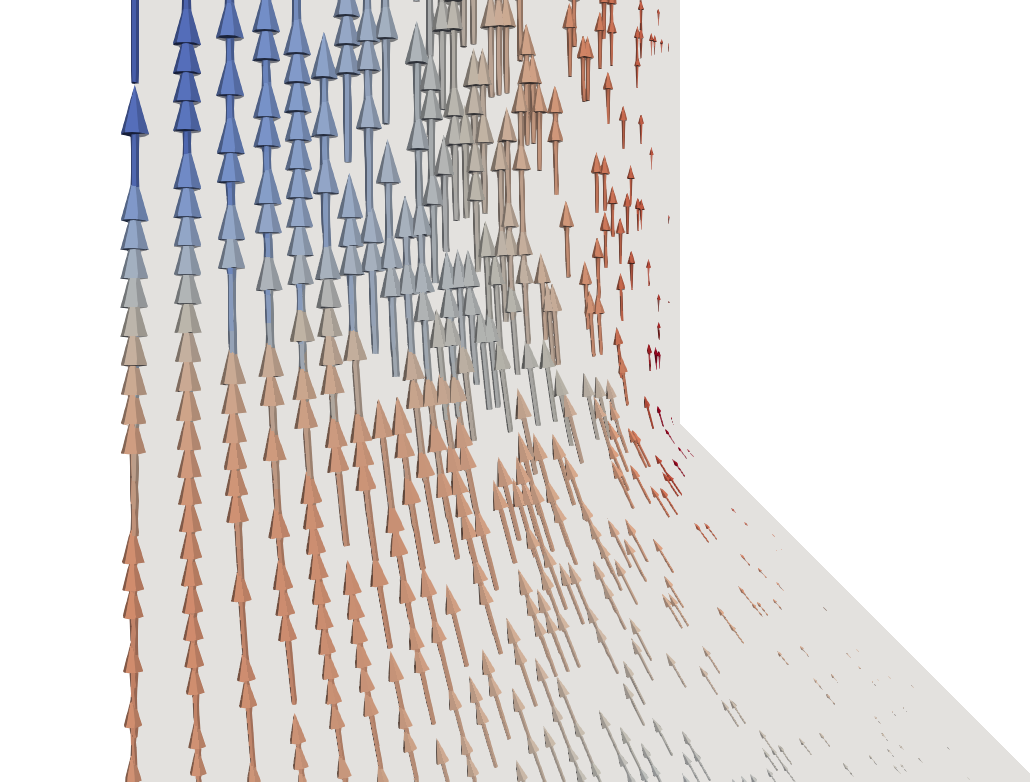
\includegraphics[trim = 0mm 0mm 0mm 0mm, clip, width=1.955in]{./images/45_stress_vector.png}
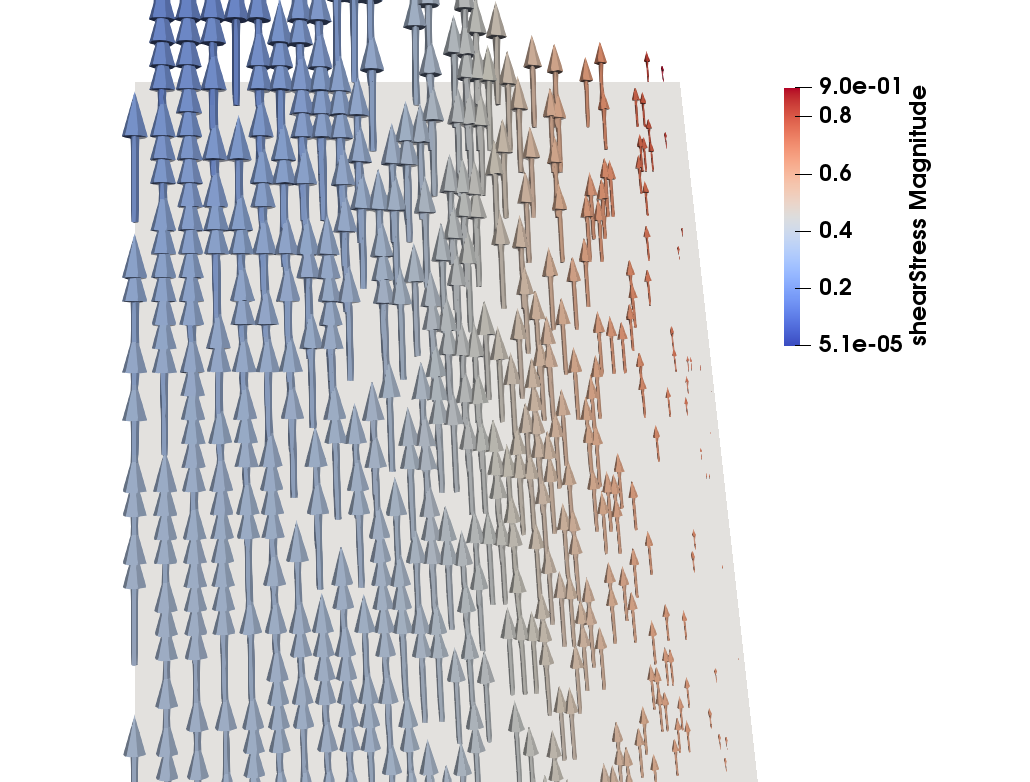
\includegraphics[trim = 0mm 0mm 0mm 0mm, clip, width=1.955in]{./images/tapered_stress_vector.png}
\end{frame}


% Appendix III ---------------------------
\begin{frame}[plain,noframenumbering]{Appendix III}
\begin{itemize}
    \item Model validation imbalances:
\end{itemize}
\vspace{3mm}
\centering
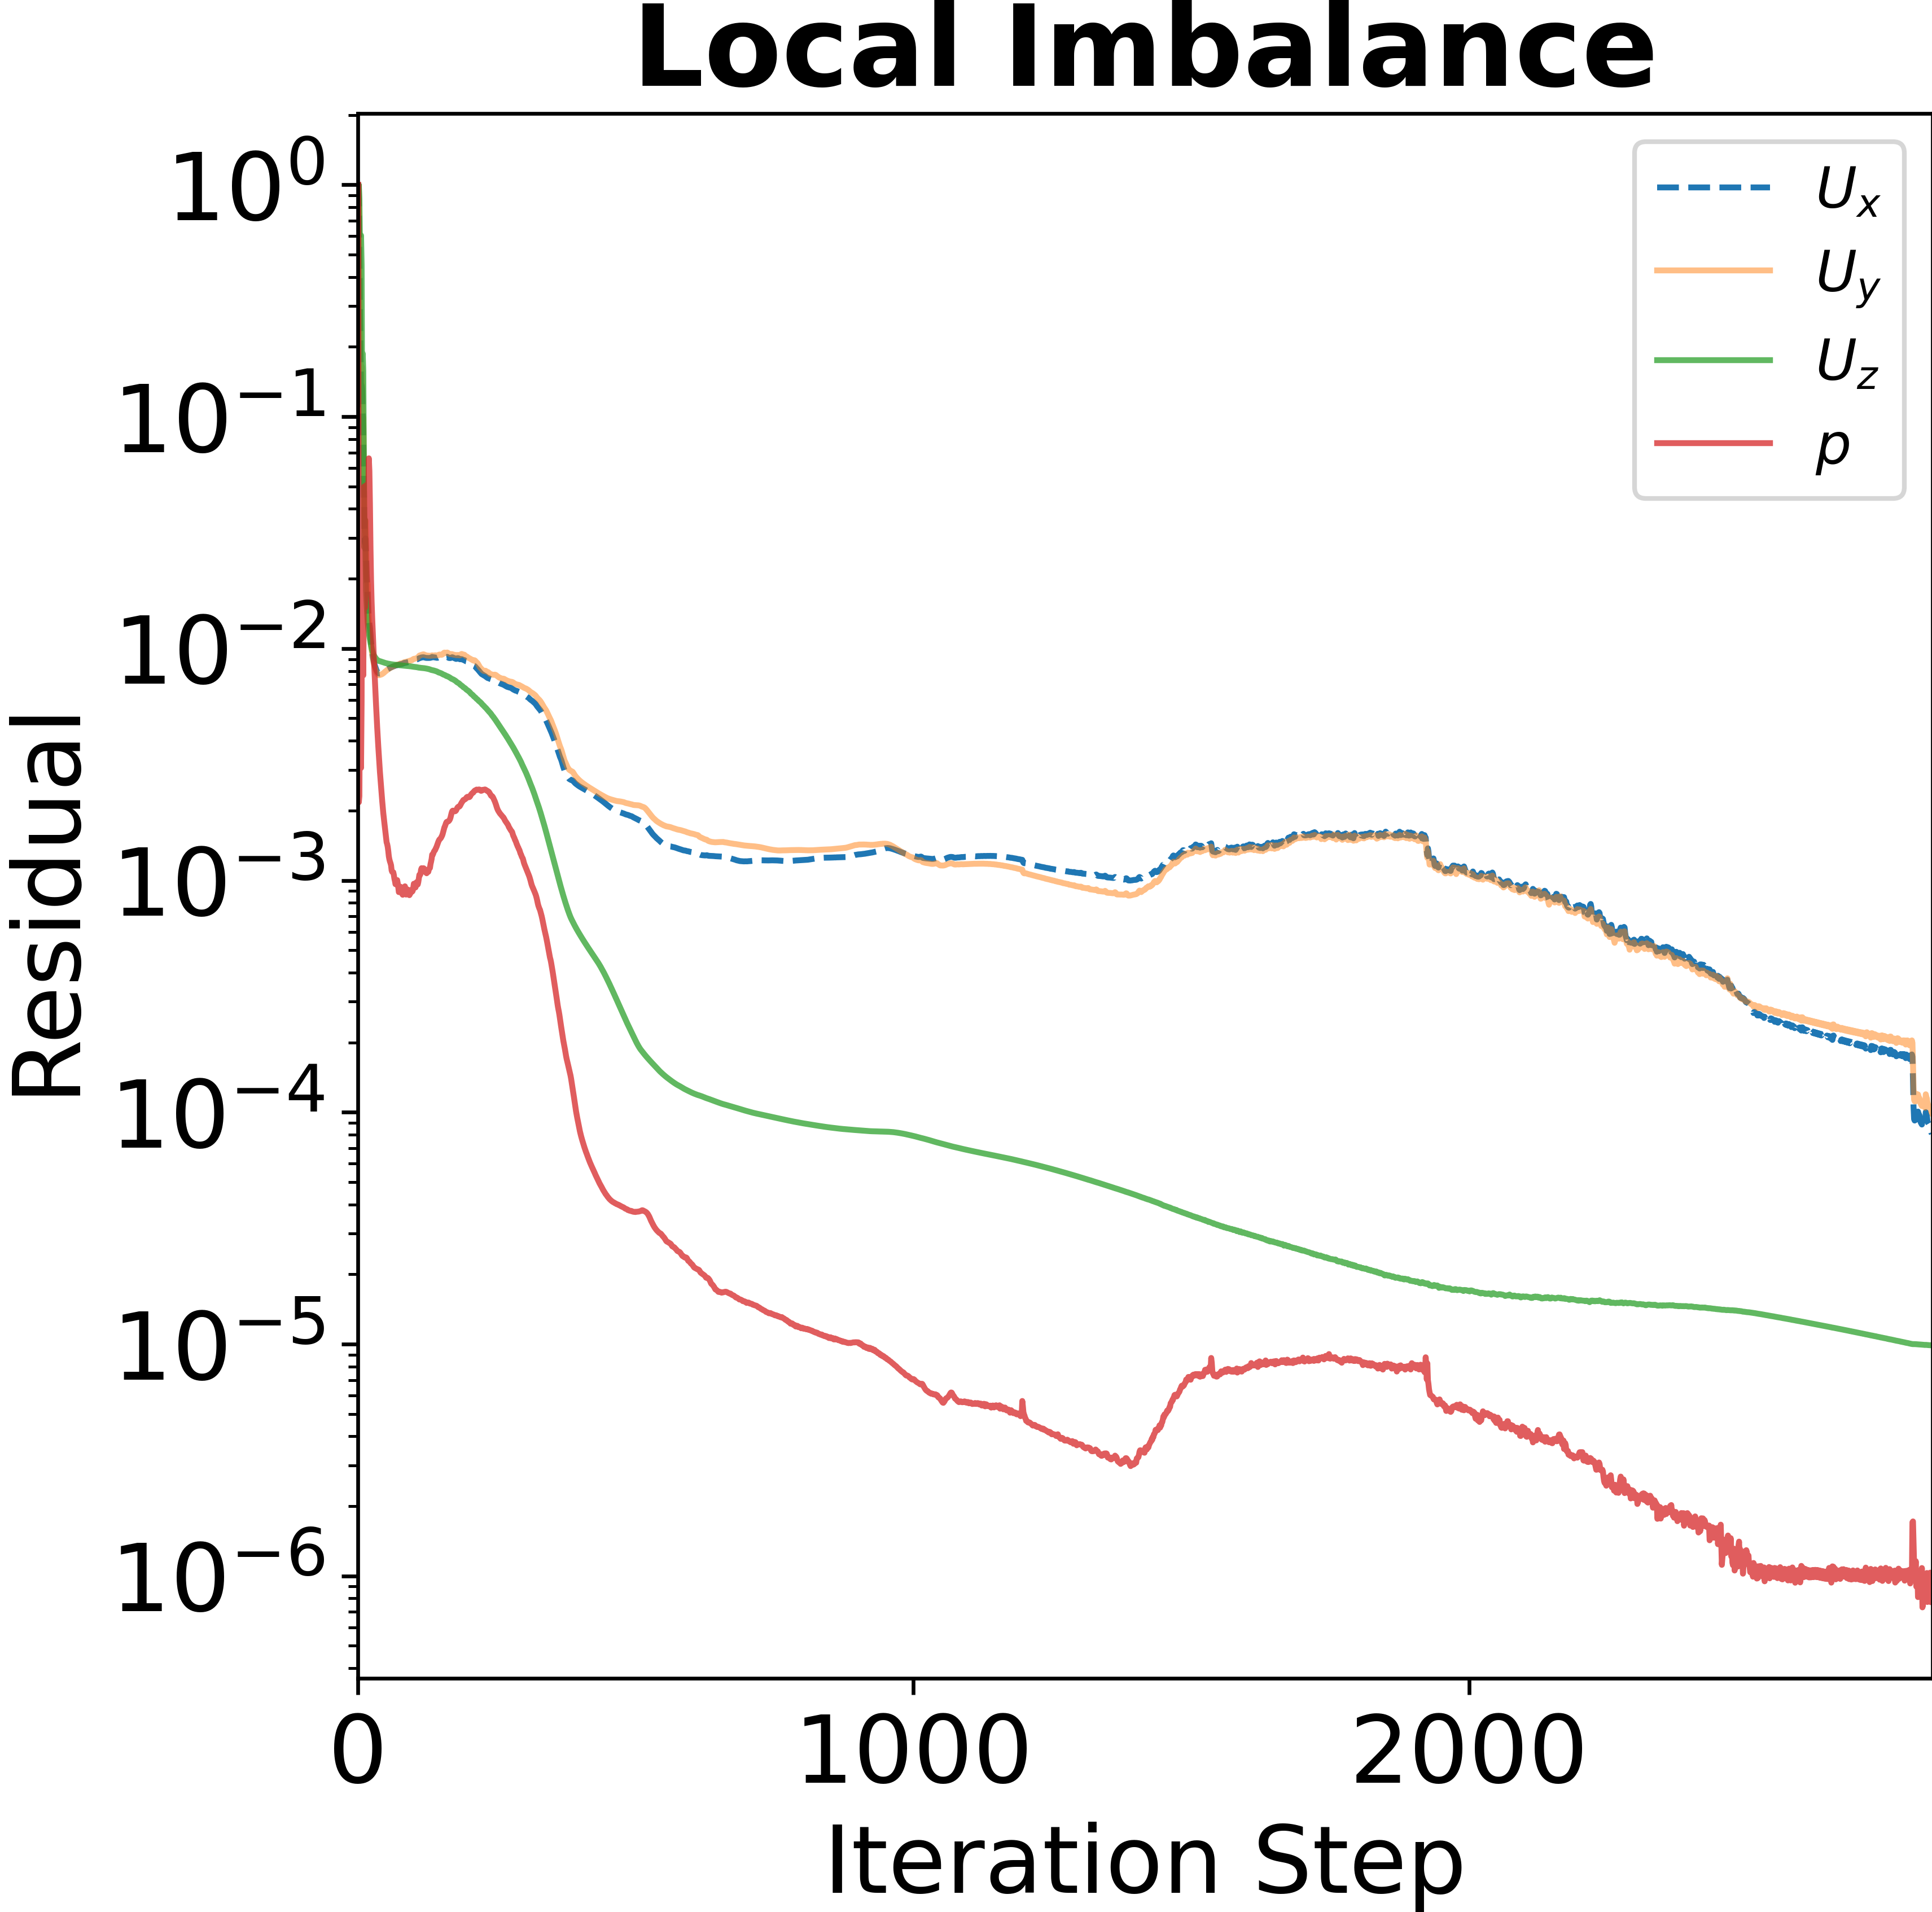
\includegraphics[trim = 0mm 0mm 0mm 0mm, clip, width=2.2in]{./images/residuals.png}
\hspace{3mm}
\centering
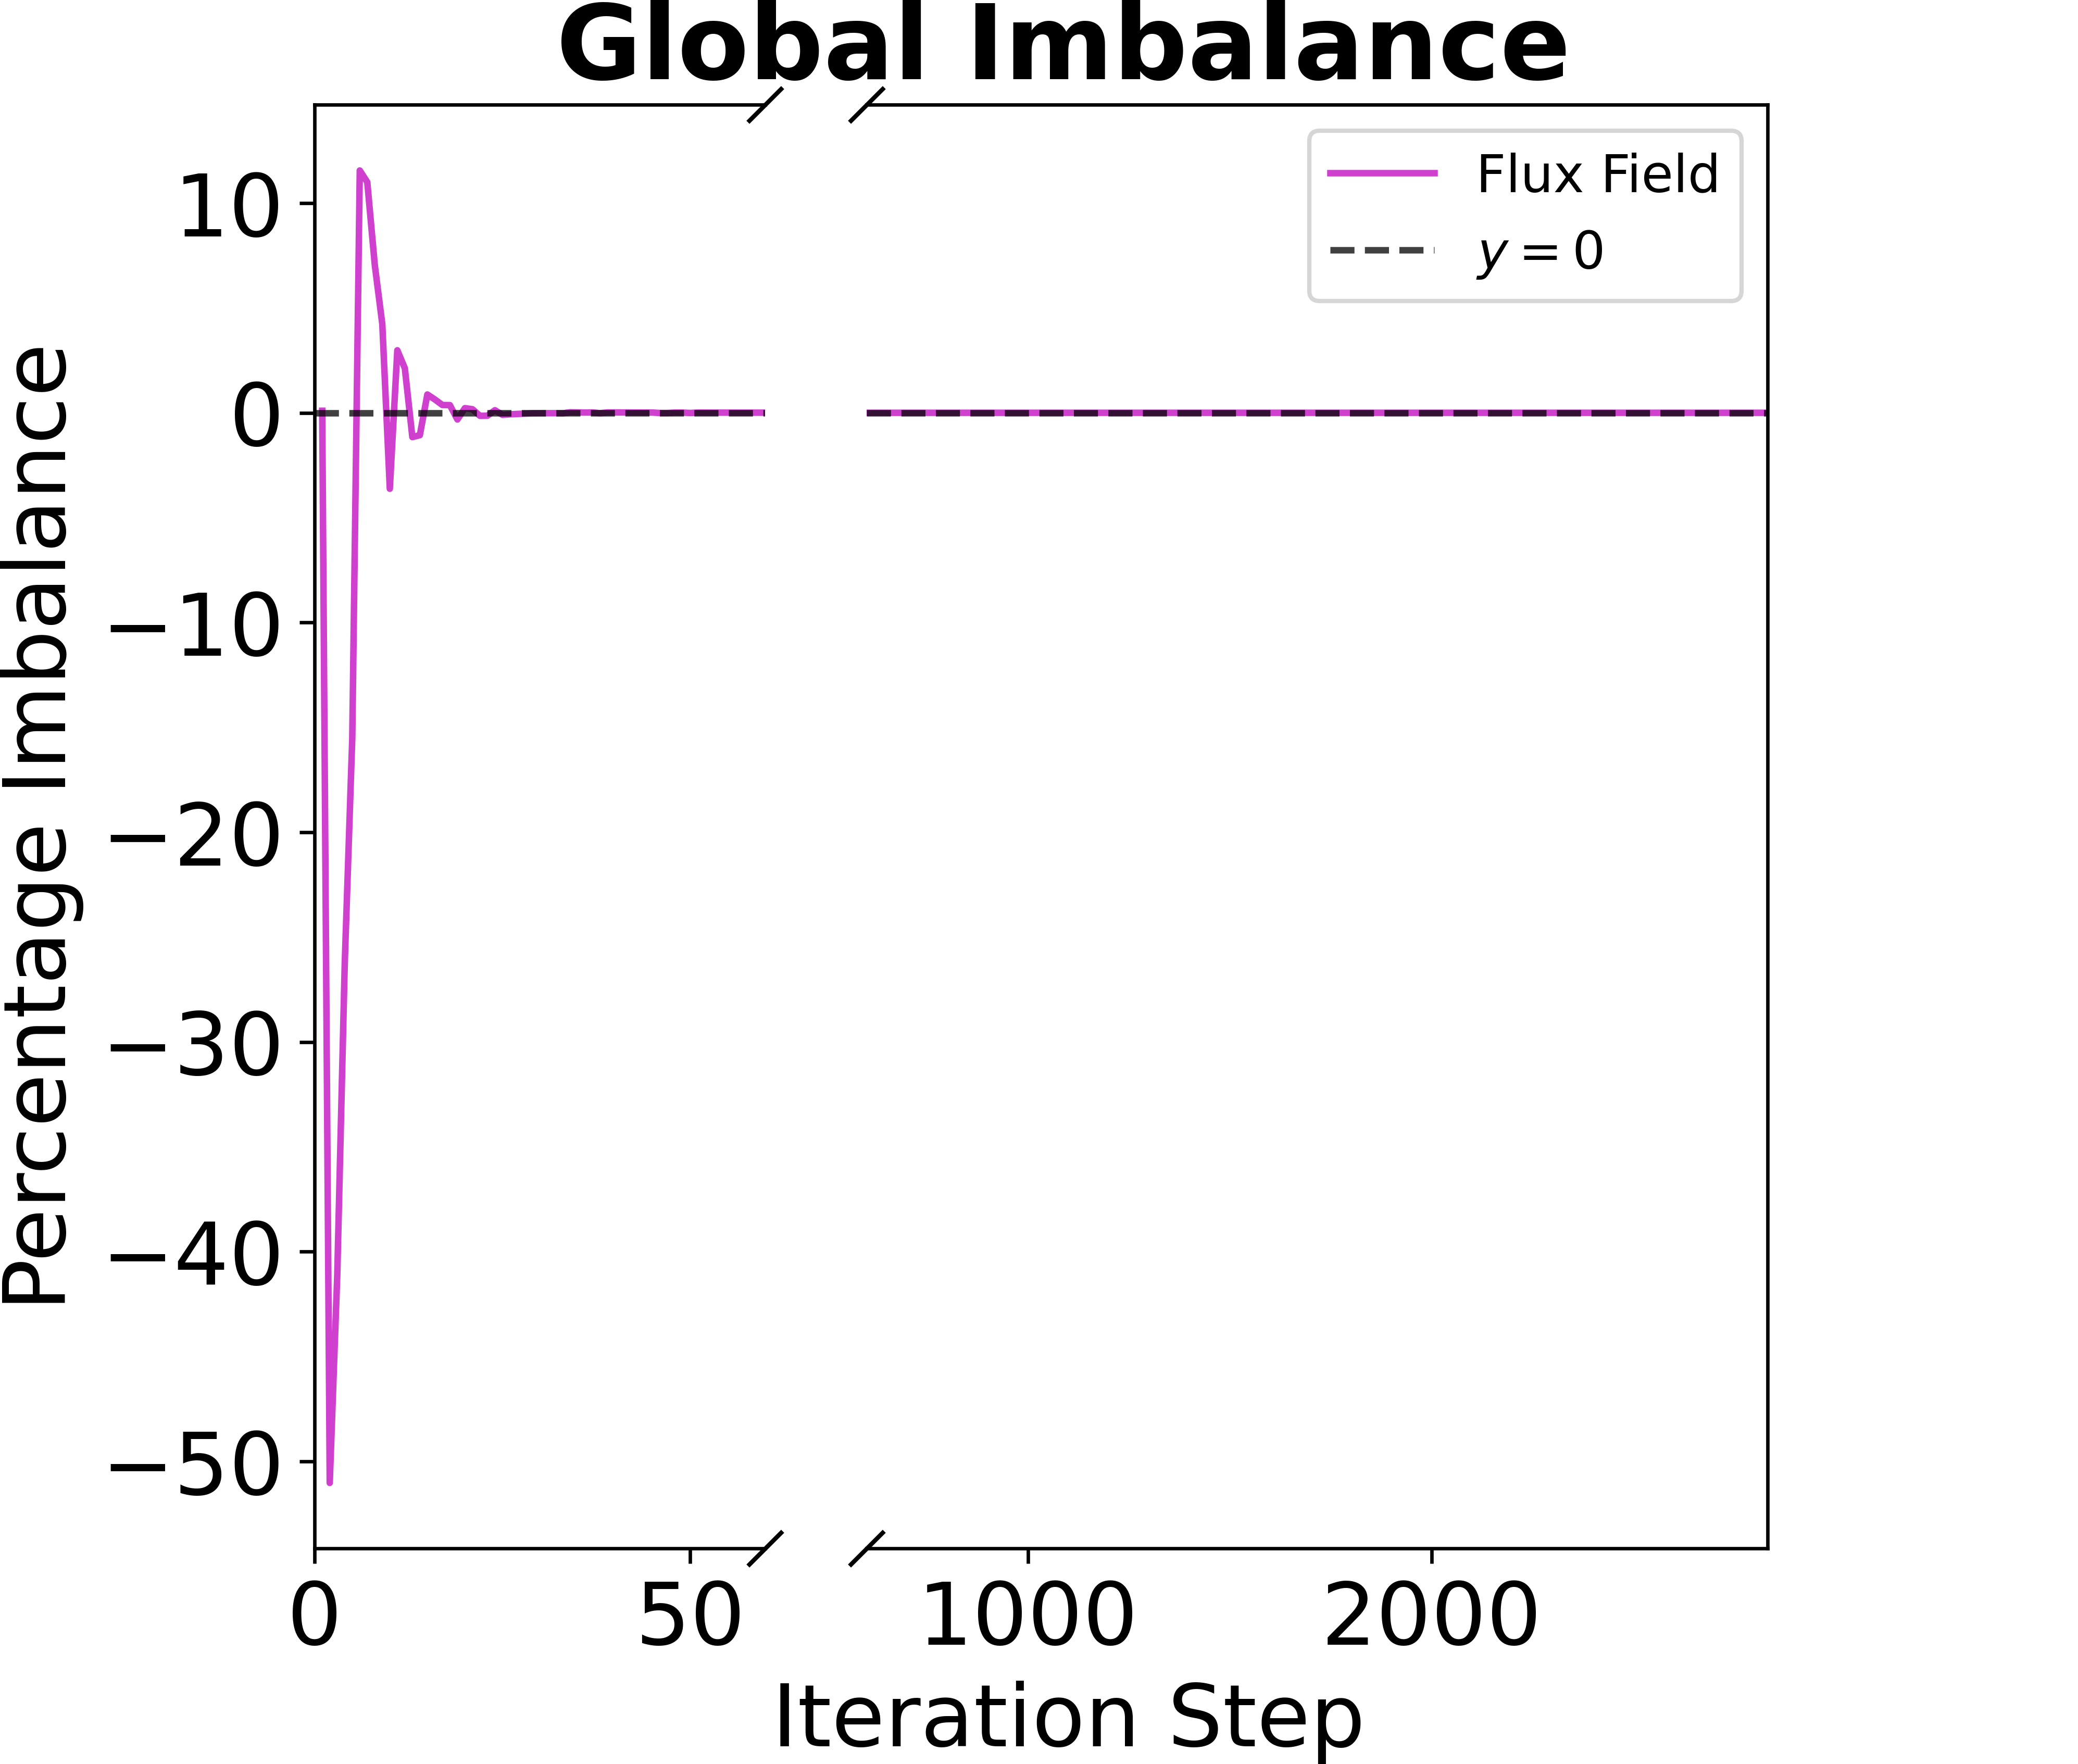
\includegraphics[trim = 0mm 0mm 0mm 0mm, clip, width=2.545in]{./images/global_imbalance.png}
\end{frame}


% Appendix IV ---------------------------
\begin{frame}[plain,noframenumbering]{Appendix IV}
\begin{itemize}
    \item Model validation stress contour plots of analytical solution (Pa) \& simulation (kPa):
\end{itemize}
\vspace{3mm}
\centering
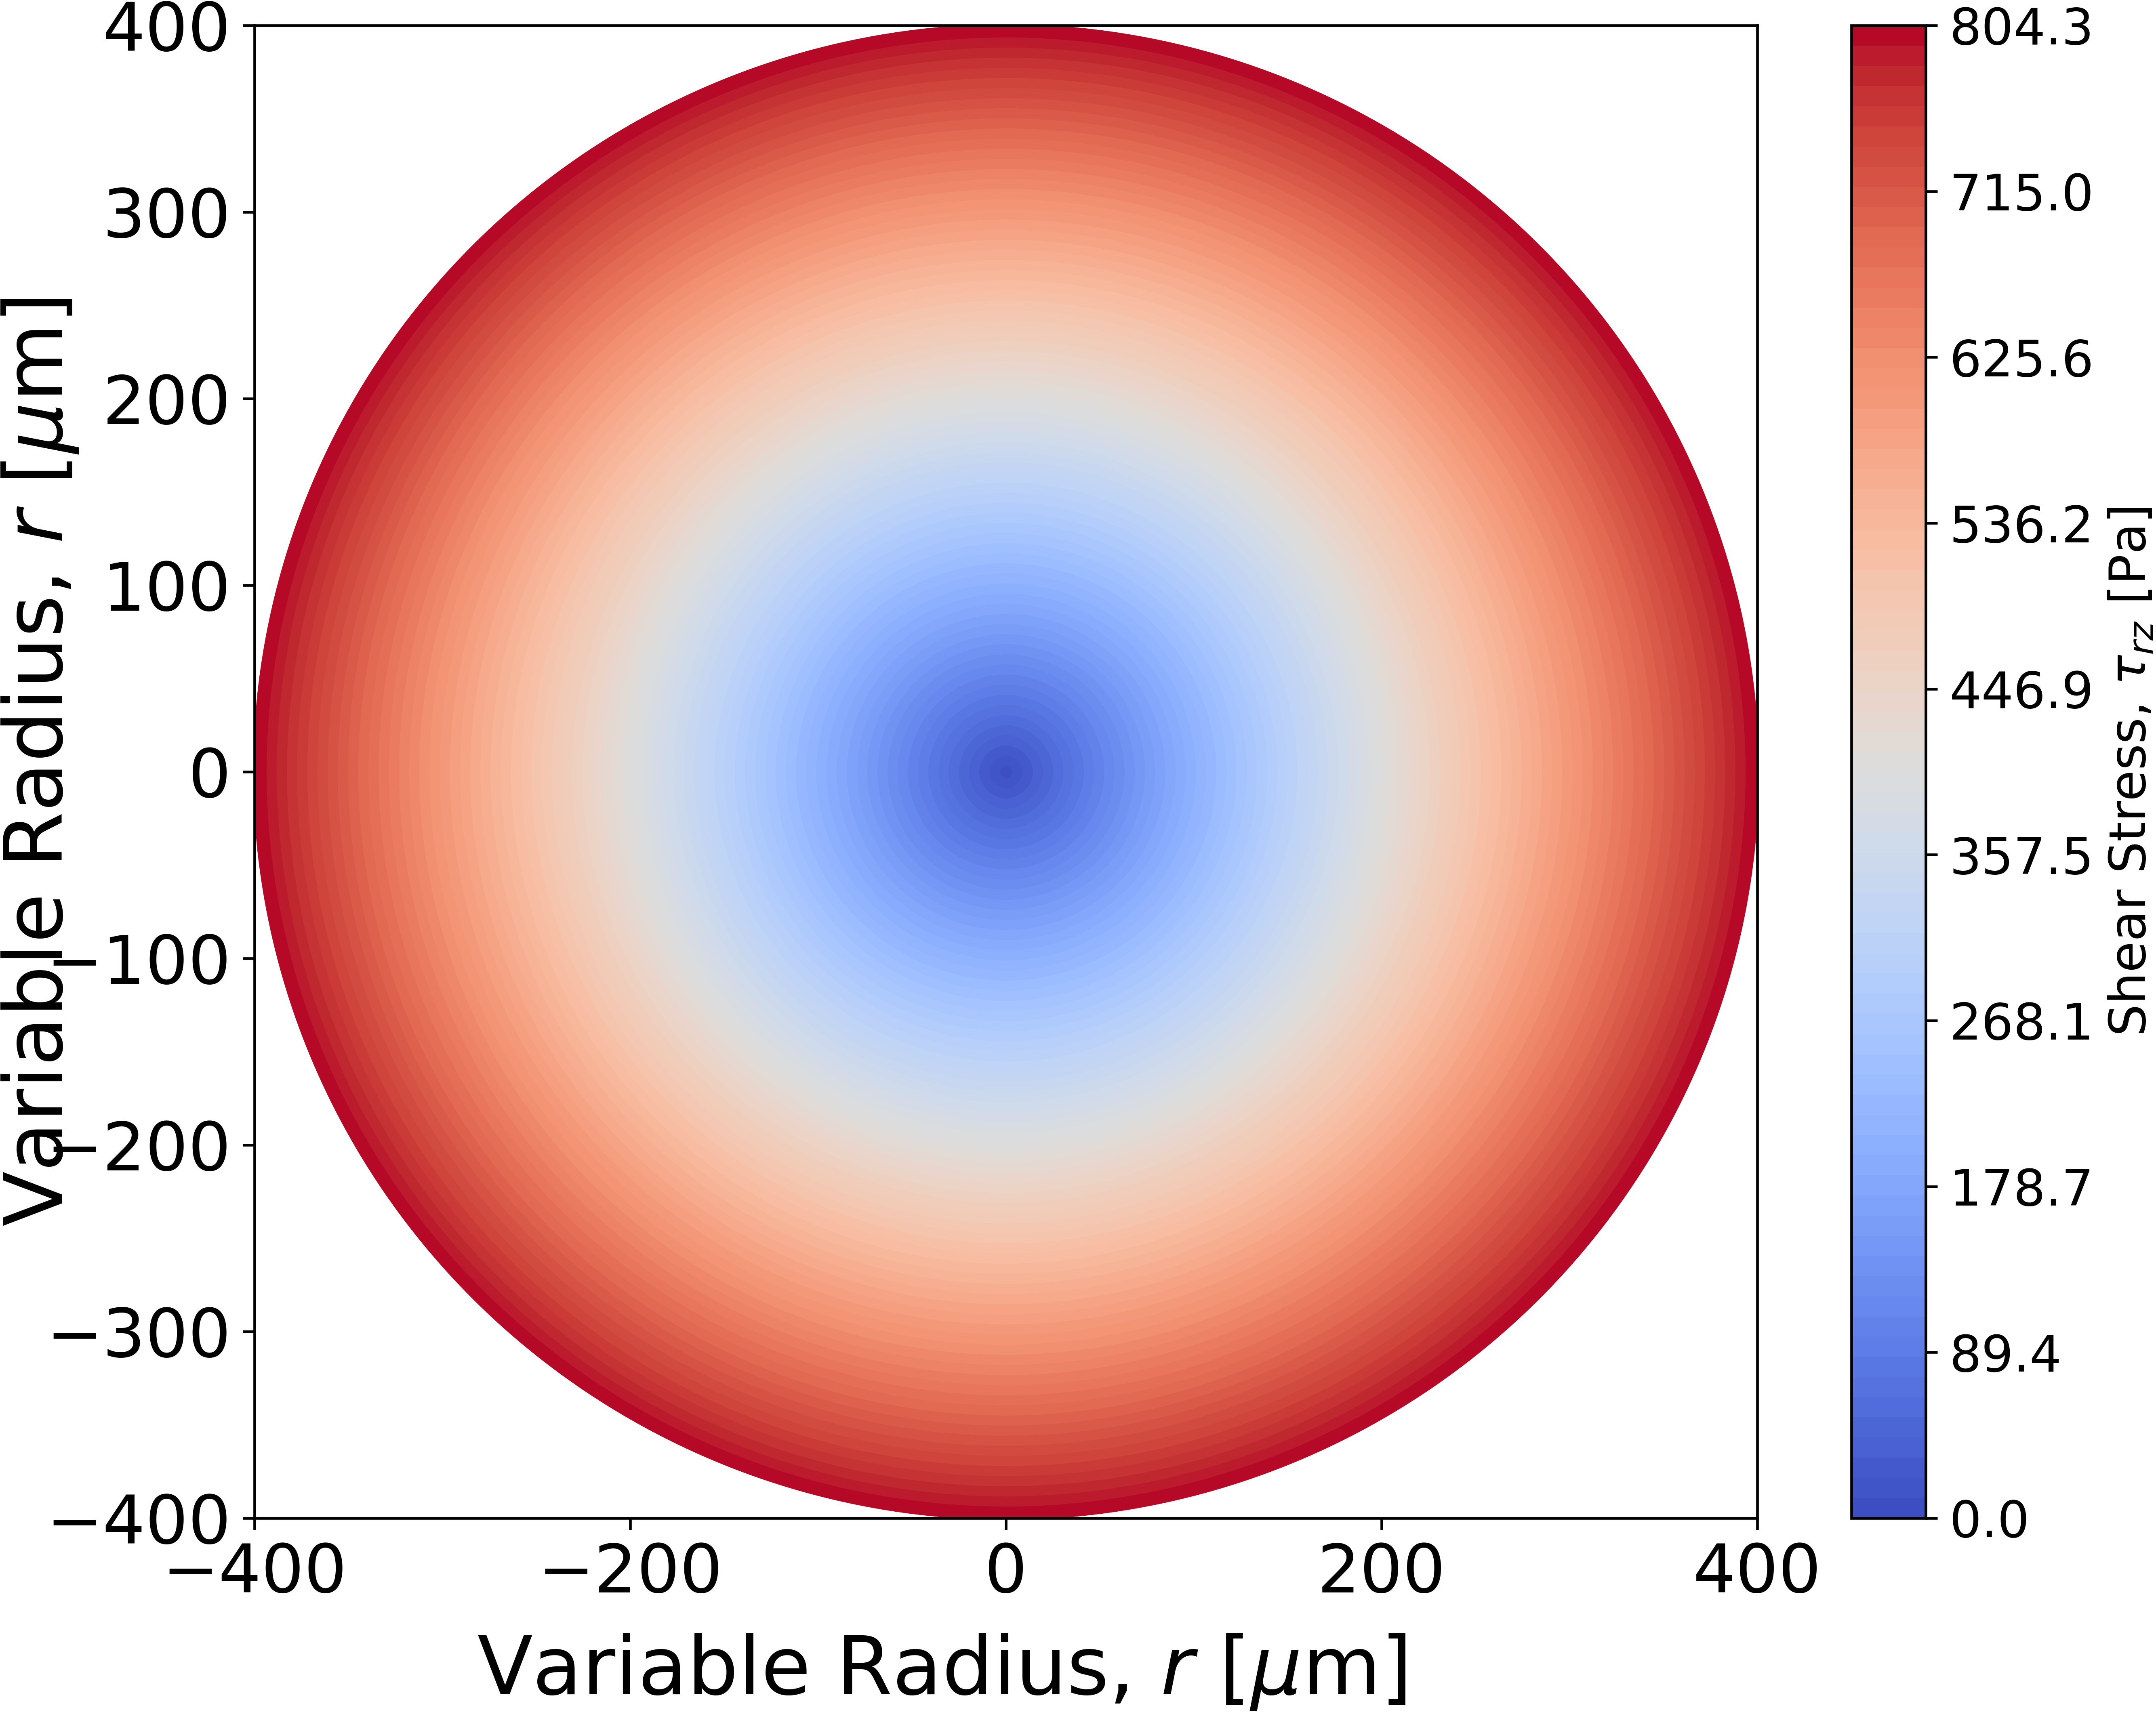
\includegraphics[trim = 0mm 0mm 0mm 0mm, clip, width=2.9in]{./images/full_cut_contour.png}
\centering
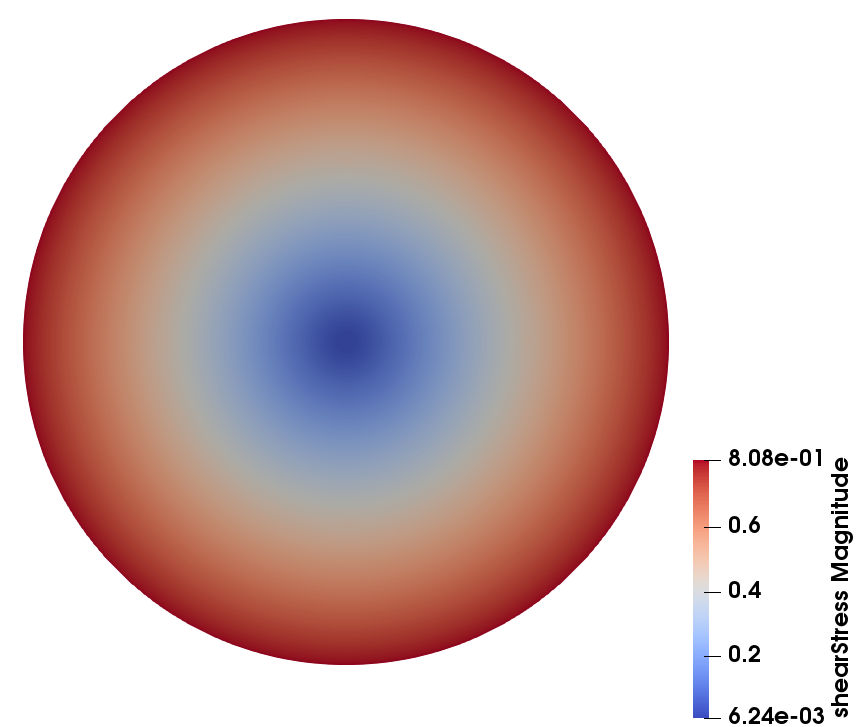
\includegraphics[trim = 0mm 0mm 0mm 0mm, clip, width=2.9in]{./images/simulation_contour.png}
\end{frame}


% Appendix V ---------------------------
\begin{frame}[plain,noframenumbering]{Appendix V}
\begin{itemize}
    \item Meshes need to be refined near wall boundaries to capture high-velocity gradients:
\end{itemize}
\vspace{2mm}
\begin{columns}
\column{.5\textwidth}
\centering
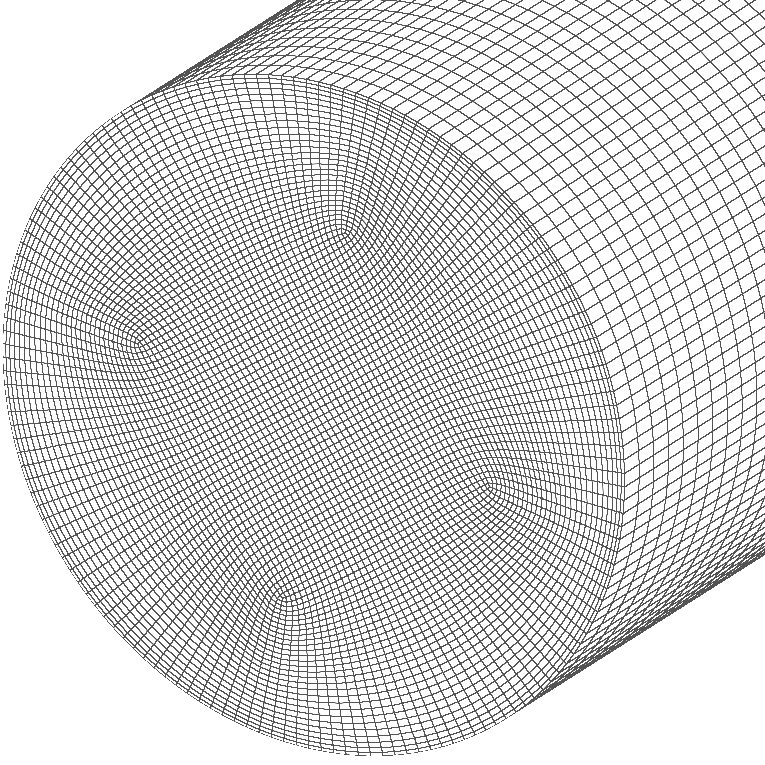
\includegraphics[trim = 0mm 0mm 0mm 0mm, clip, width=2.6in]{./images/mesh_validation.png}
\column{.5\textwidth}
\centering
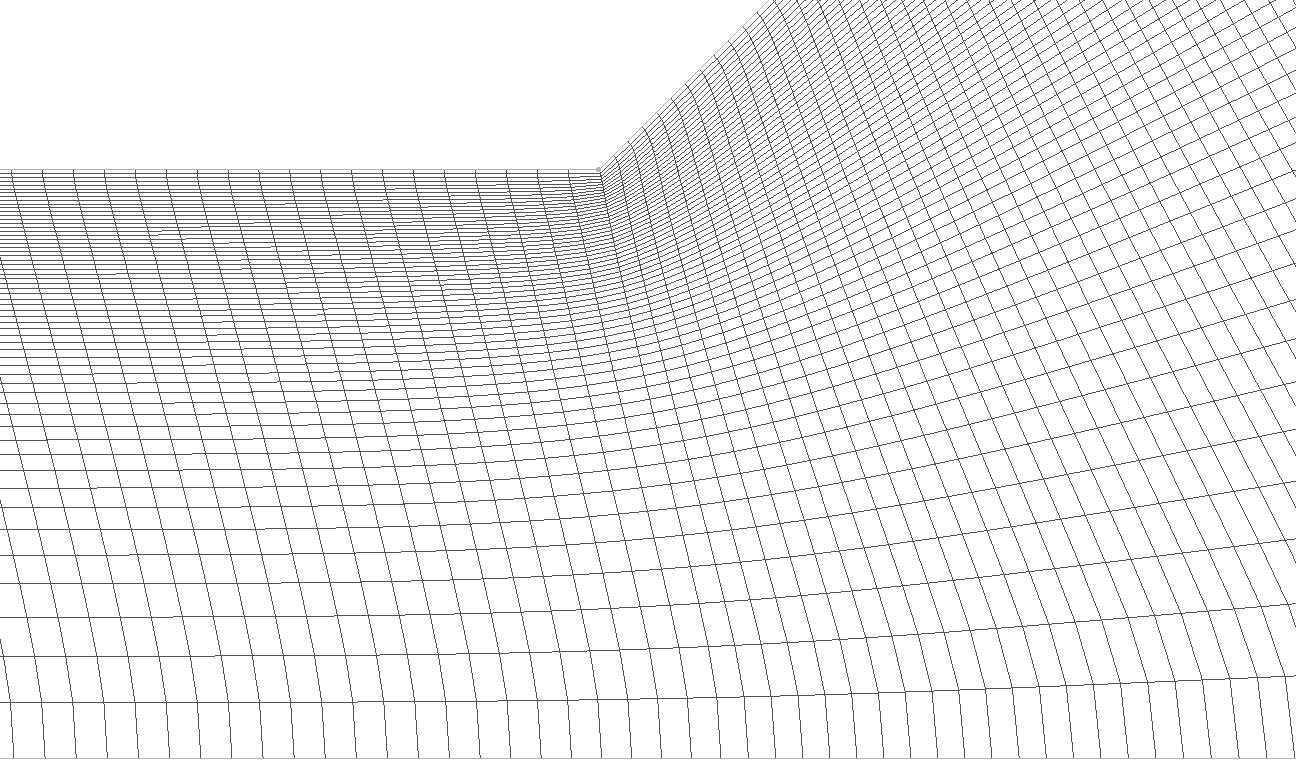
\includegraphics[trim = 0mm 0mm 0mm 0mm, clip, width=2.6in]{./images/mesh_simulation.png}
\end{columns}
\end{frame}


% Appendix VI ---------------------------
\begin{frame}[plain,noframenumbering]{Appendix VI}
\begin{itemize}
    \item Mesh independency study for the 45$^{\circ}$ cylindrical needle at 25 $^{\circ}$C:
\end{itemize}
\begin{figure}
    \centering
    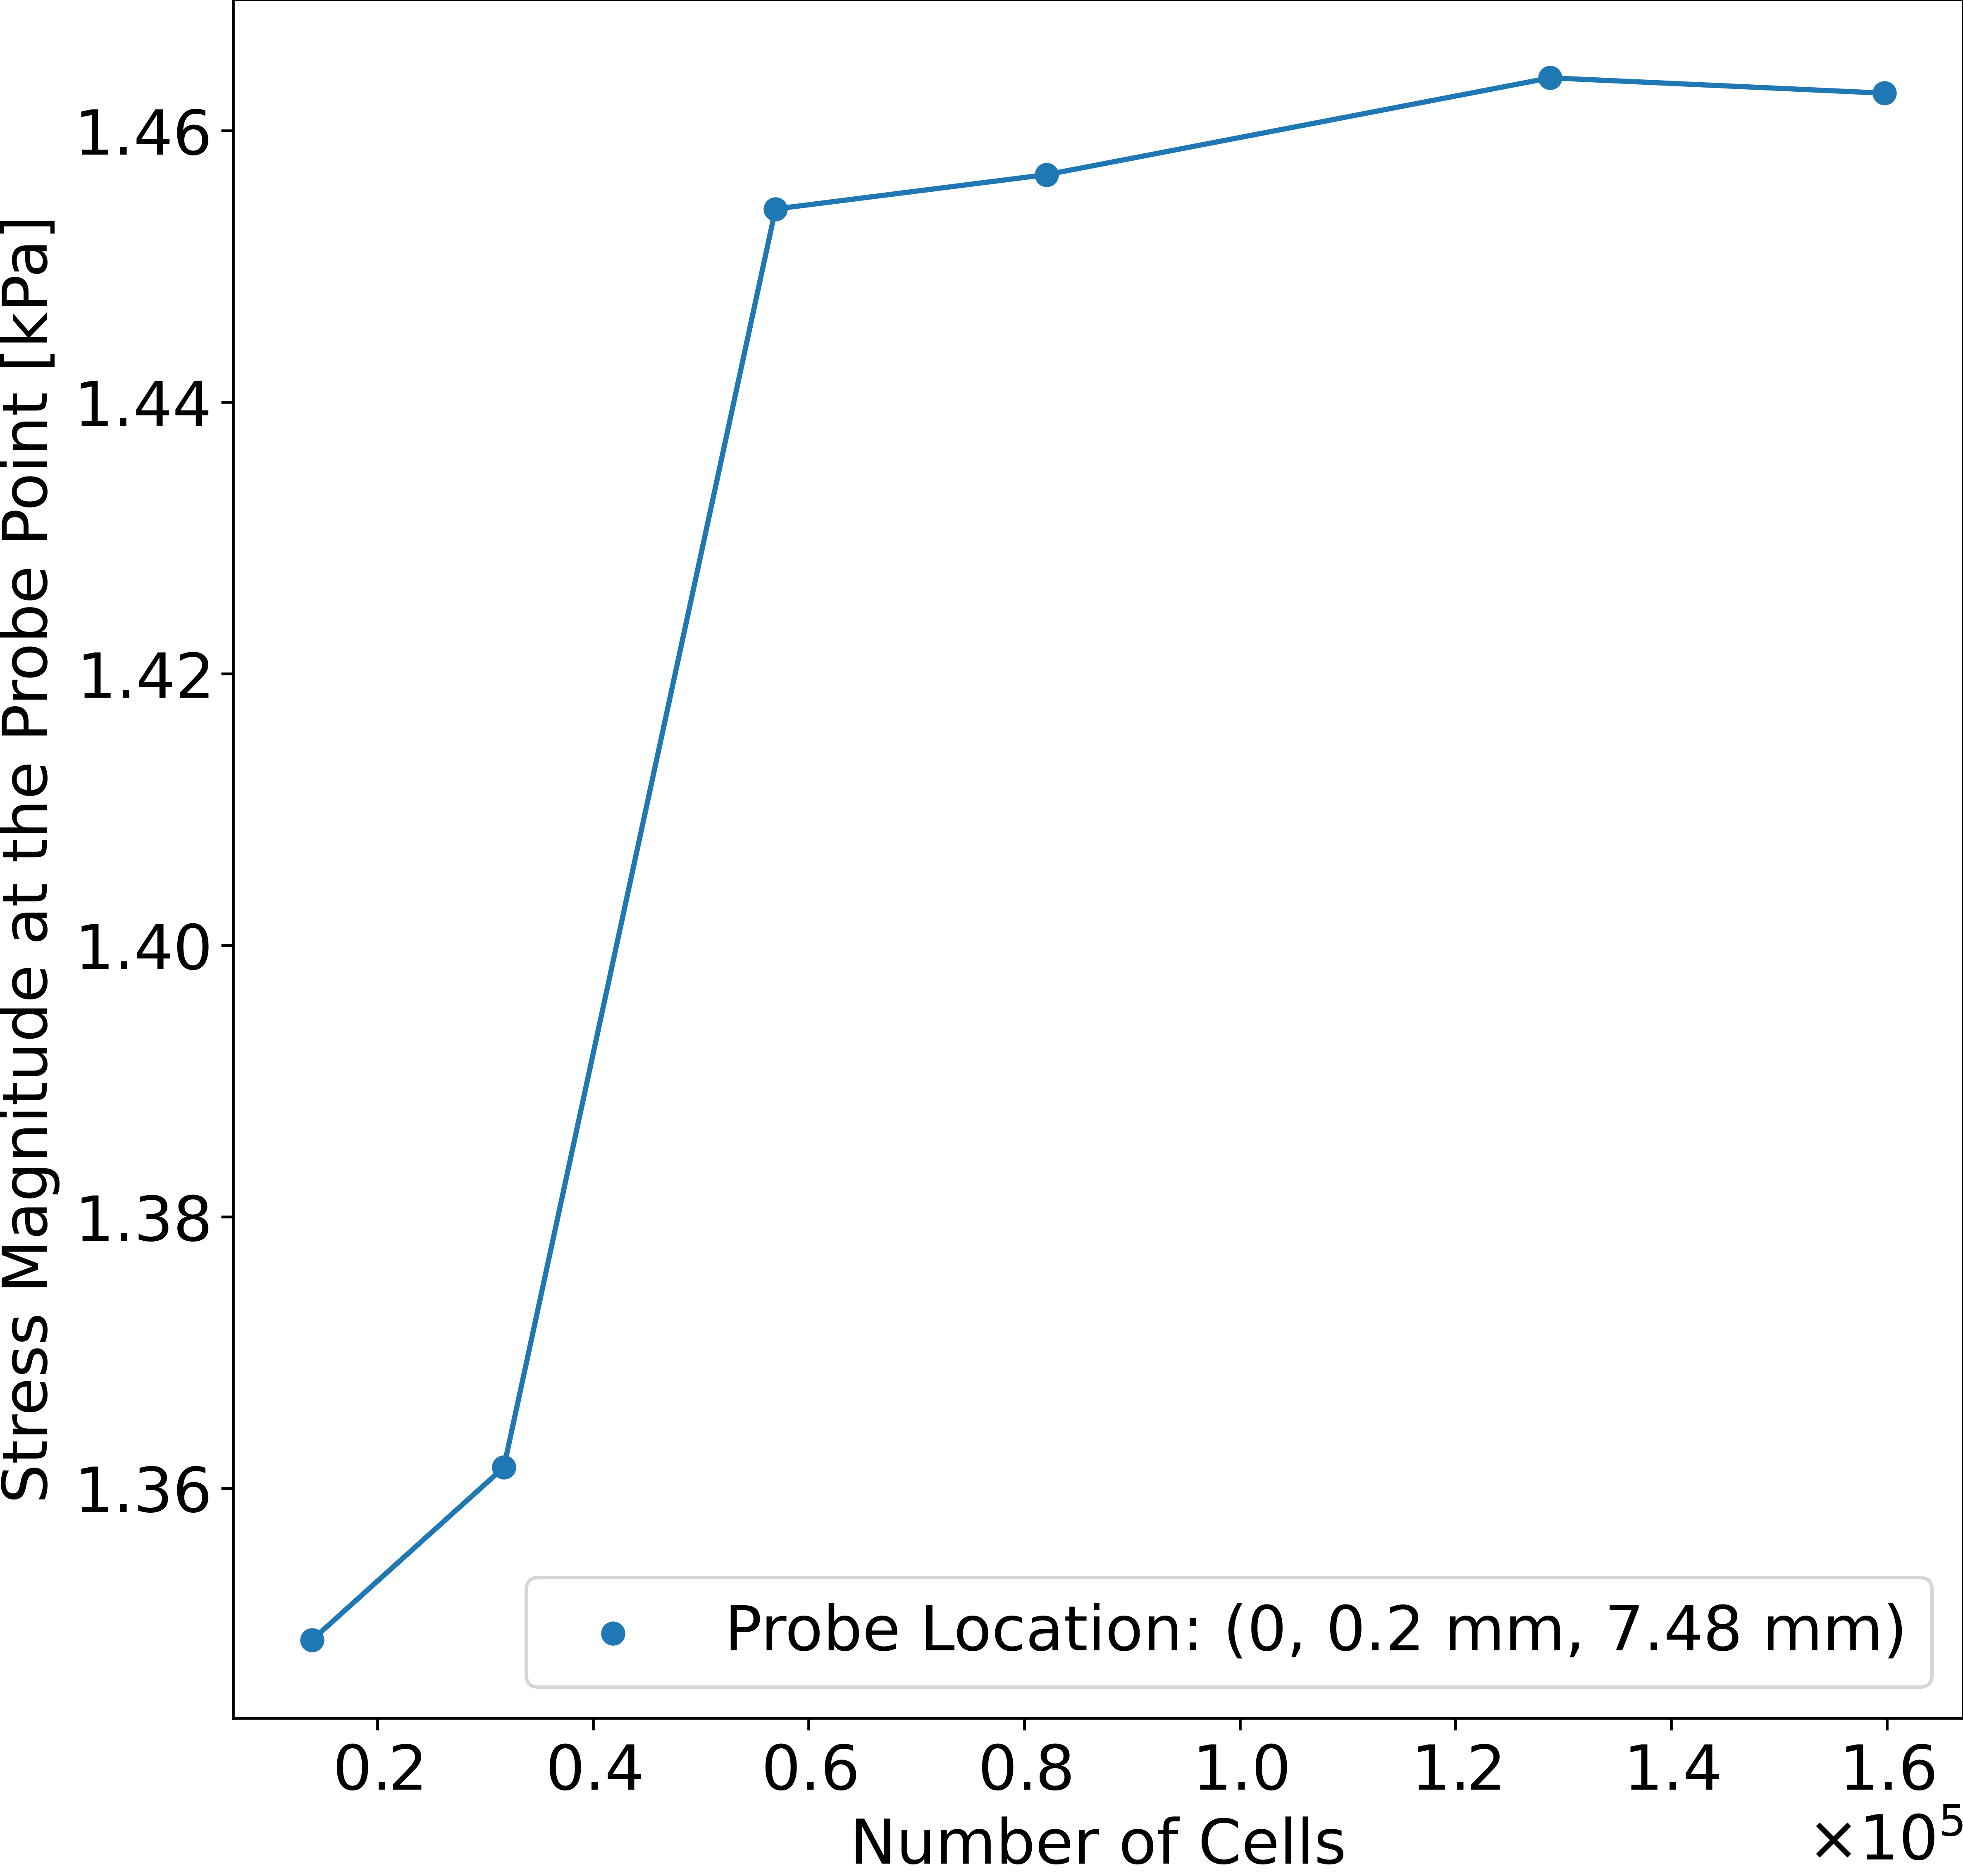
\includegraphics[trim = 0mm 0mm 0mm 0mm, clip, width=2.5in]{./images/MDT_45_25C.png}
\end{figure}
\end{frame}


% Appendix VII ---------------------------


%\fi

\end{document}